%%%%%%%%%%%%%%%%%%%%%%%%%%%%%%%%%%%%%%%%%%%%%%%%%%%%%%%%%%%%%%%%%%%%%%%%%%%%%%%%
\section{Supplementary material}
%%%%%%%%%%%%%%%%%%%%%%%%%%%%%%%%%%%%%%%%%%%%%%%%%%%%%%%%%%%%%%%%%%%%%%%%%%%%%%%%

This supplementary material contains additional facets of \verb;pirouette;, such as the installation of the package, an overview of
pirouette's main functions and a guide for empiricists, based on multiple experiments
that are shown here as well.

For these experiments, we limited the number of replicates by time, 
aiming at a duration of
24 hours per setting, when run on the Peregrine computer cluster of the
University of Groningen. Due to this, for example, a run of 40 taxa only
has 6 replicates, because one run takes 4 hours. For all experiments, the intermediate results can all be downloaded 
from their respective websites, which is approximately 5 gigabyte in total.

All the figures shown in this section are shown without any aesthetical modifications, with the exception that the arrangement
of the sub-figures in subsection \ref{subsec:main_example},
where we aligned parts of the figure by hand.

Here is an overview of the various sections:

\begin{itemize}
  \item{
    subsection \ref{subsec:guidelines}: guidelines for empiricists
  }
  \item{
    subsection \ref{subsec:installation}: installation
  }
  \item{
    subsection \ref{subsec:resources}: resources, such as 
    website, tutorials, packages used, bug reporting and contributing
  }
  \item{
    subsection \ref{subsec:citation}: citation of pirouette
  }
  \item{
    subsection \ref{subsec:main_functions}: main functions
  }
  \item{
    subsection \ref{subsec:main_example}: code, extra figures and
    diagnostics regarding the main example.
  }
  \item{
    subsection \ref{subsec:distribution}: the result of using 
    multiple trees, as generated by the
    same stochastic process as the main example
  }
  \item{
    subsection \ref{subsec:n_taxa}: the effect of the number
    of taxa
  }
  \item{
    subsection \ref{subsec:n_nucleotides}: the effect of the DNA
    alignment sequence length
  }
  \item{
    subsection \ref{subsec:simplest_correct_parameterization} shows the
    effect when doing an inference in the simplest use case
  }
  \item{
    subsection \ref{subsec:under_parameterization} shows the
    effect when doing an inference with an under-parameterization
  }
  \item{
    subsection \ref{subsec:different_n_mutations} shows the
    effect when the twin alignment is allowed to have a different
    number of mutations
  }
  \item{
    subsection \ref{subsec:mutation_rate} shows the
    effect of different mutation rates
  }
\end{itemize}

%%%%%%%%%%%%%%%%%%%%%%%%%%%%%%%%%%%%%%%%%%%%%%%%%%%%%%%%%%%%%%%%%%%%%%%%%%%%%%%%
\subsection{Guidelines for empiricists}
\label{subsec:guidelines}
%%%%%%%%%%%%%%%%%%%%%%%%%%%%%%%%%%%%%%%%%%%%%%%%%%%%%%%%%%%%%%%%%%%%%%%%%%%%%%%%

From the experiments shown below, we composed some rough guidelines.
These guidelines should be treated as preliminary results, as
the total runtime of these experiments is 'only' 19 days.

\begin{itemize}
  \item{
    The use of 20 replicates results in decent plots.
  }
  \item{
    The use of more taxa increases the inference error
  }
  \item{
    The use of longer DNA sequences decreases the inference error.
  }
  \item{
    When we do not impose the same number of mutations between true and twin alignment, we observe a difference in the error distributions with respect to the standard case (presented in the main text) where they are forced to have the same number of mutations.
  }
  \item{
    Using a mutation rate less than 1.0 / crown age, decreases the
    inference error. We predict this will increase the error in the parameter
    estimation.
  }
\end{itemize}

%%%%%%%%%%%%%%%%%%%%%%%%%%%%%%%%%%%%%%%%%%%%%%%%%%%%%%%%%%%%%%%%%%%%%%%%%%%%%%%%
\subsection{Installation}
\label{subsec:installation}
%%%%%%%%%%%%%%%%%%%%%%%%%%%%%%%%%%%%%%%%%%%%%%%%%%%%%%%%%%%%%%%%%%%%%%%%%%%%%%%%

\verb;pirouette; will be made available on CRAN from which 
it can then be easily installed:
\begin{lstlisting}[language=R, floatplacement=ht, frame=single]
install.packages("pirouette")
\end{lstlisting}

Until it is on CRAN, and for the most up-to-date version, 
one can download and install the package from \verb;pirouette;'s GitHub 
repository. We do first need the \verb;mcbette; and \verb;nodeSub; packages:
\begin{lstlisting}[
    language = R,
    floatplacement = ht,
    frame = single
]
remotes::install_github(
  "richelbilderbeek/mcbette"
)
remotes::install_github(
  "thijsjanzen/nodeSub"
)
\end{lstlisting}

Now we can install \verb;pirouette;:
\begin{lstlisting}[
    language = R,
    floatplacement = ht,
    frame = single
]
remotes::install_github(
  "richelbilderbeek/pirouette"
)
\end{lstlisting}
which also installs its dependencies from CRAN.

To start using \verb;pirouette;, 
load its functions in the global namespace first:
\begin{lstlisting}[language=R, floatplacement=ht, frame=single]
library(pirouette)
\end{lstlisting}
Because \verb;pirouette; calls BEAST2, BEAST2 must be installed. 
This can be done from within R, using:
\begin{lstlisting}[language=R, floatplacement=ht, frame=single]
beastier::install_beast2()
\end{lstlisting}
For the option to select the best candidate model,
\verb;pirouette; needs the "NS" BEAST2 package [\cite{russel2019model}].
It can be installed from within R, using:
\begin{lstlisting}[language=R, floatplacement=ht, frame=single]
mauricer::install_beast2_pkg("NS")
\end{lstlisting}

%%%%%%%%%%%%%%%%%%%%%%%%%%%%%%%%%%%%%%%%%%%%%%%%%%%%%%%%%%%%%%%%%%%%%%%%%%%%%%%%
\subsection{Resources}
\label{subsec:resources}
%%%%%%%%%%%%%%%%%%%%%%%%%%%%%%%%%%%%%%%%%%%%%%%%%%%%%%%%%%%%%%%%%%%%%%%%%%%%%%%%

\verb;pirouette; is free, libre and open source software available at 
\url{http://github.com/richelbilderbeek/pirouette},
licensed under the GNU General Public License version 3.
\verb;pirouette; depends on multiple packages, which are:
\verb;ape; [\cite{ape}],
\verb;assertive; [\cite{assertive}],
\verb;babette; [\cite{bilderbeek2018babette}],
\verb;DDD; [\cite{DDD}],
\verb;devtools; [\cite{devtools}],
\verb;dplyr; [\cite{dplyr}],
\verb;ggplot2; [\cite{ggplot2}],
\verb;knitr; [\cite{knitr}],
\verb;lintr; [\cite{lintr}],
\verb;magrittr; [\cite{magrittr}],
\verb;mcbette; [\cite{mcbette}],
\verb;nLTT; [\cite{nLTT}],
\verb;phangorn; [\cite{phangorn}],
\verb;phytools; [\cite{phytools}],
\verb;plyr; [\cite{plyr}],
\verb;rappdirs; [\cite{rappdirs}],
\verb;rmarkdown; [\cite{rmarkdown}],
\verb;Rmpfr; [\cite{Rmpfr}],
\verb;stringr; [\cite{stringr}],
\verb;TESS; [\cite{TESS}],
\verb;testit; [\cite{testit}], 
\verb;testthat; [\cite{testthat}] and
\verb;tidyr; [\cite{tidyr}].

\verb;pirouette;'s development takes place on GitHub,
\url{https://github.com/richelbilderbeek/pirouette},
which allows submitting bug reports, requesting features, 
and adding code. To improve quality, \verb;pirouette; 
uses a continuous integration service, has a code coverage of above 95\%
and enforces the most commonly used R style guide [\cite{style_guide}].

\verb;pirouette;'s is extensively documented on its website,
its documentation and its vignettes.
The \verb;pirouette; website is a good starting point to learn
how to use \verb;pirouette;, as it links to tutorials and videos.
The \verb;pirouette; package documentation describes
all functions and liberally links to related functions.
All exported functions show a minimal example as part of their documentation.
The \verb;pirouette; vignette demonstrates extensively how 
to use \verb;pirouette; in a more informally written way. 

The code used in this article and more examples that are periodically 
tested, can be found at 
\url{https://github.com/richelbilderbeek/pirouette_examples}. 

%%%%%%%%%%%%%%%%%%%%%%%%%%%%%%%%%%%%%%%%%%%%%%%%%%%%%%%%%%%%%%%%%%%%%%%%%%%%%%%%
\subsection{Citation of pirouette}
\label{subsec:citation}
%%%%%%%%%%%%%%%%%%%%%%%%%%%%%%%%%%%%%%%%%%%%%%%%%%%%%%%%%%%%%%%%%%%%%%%%%%%%%%%%

To cite \verb;pirouette; this article from within R, use:

\begin{lstlisting}[language=R]
> citation("pirouette")
\end{lstlisting}

%%%%%%%%%%%%%%%%%%%%%%%%%%%%%%%%%%%%%%%%%%%%%%%%%%%%%%%%%%%%%%%%%%%%%%%%%%%%%%%%
\subsection{Main functions}
\label{subsec:main_functions}
%%%%%%%%%%%%%%%%%%%%%%%%%%%%%%%%%%%%%%%%%%%%%%%%%%%%%%%%%%%%%%%%%%%%%%%%%%%%%%%%

An overview of \verb;pirouette;'s main functions is shown in 
Table~\ref{tab:functions}. 
All \verb;pirouette;'s functions are documented,
have a useful example and sensible defaults.

%%%%%%%%%%%%%%%%%%%%%%%%%%%%%%%%%%%%%%%%%%%%%%%%%%%%%%%%%%%%%%%%%%%%%%%%%%%%%%%%
\begin{table}[h]
  \centering
  \begin{tabular}{ | l | l | l | }
    \hline
    \textbf{Name} & \textbf{Description} \\
    \hline
    \verb;pir_run; & Run \verb;pirouette; \\
    \verb;pir_plot; & Show the \verb;pirouette; results as a plot  \\
    \verb;create_pir_params; & Create the \verb;pirouette; parameters  \\
    \hline
    \verb;create_alignment_params; & Create the alignment parameters  \\
    \verb;create_twinning_params; & Create the twinning parameters  \\
    \verb;create_experiment; & Create one experiment  \\
    \verb;create_error_measure_params; & Create the error measurement parameters  \\
    \hline
  \end{tabular}
  \caption{
    \texttt{pirouette}'s main functions and description. 
  }
  \label{tab:functions}
\end{table}
%%%%%%%%%%%%%%%%%%%%%%%%%%%%%%%%%%%%%%%%%%%%%%%%%%%%%%%%%%%%%%%%%%%%%%%%%%%%%%%%

\newpage

%%%%%%%%%%%%%%%%%%%%%%%%%%%%%%%%%%%%%%%%%%%%%%%%%%%%%%%%%%%%%%%%%%%%%%%%%%%%%%%%
\subsection{Main example}
\label{subsec:main_example}
%%%%%%%%%%%%%%%%%%%%%%%%%%%%%%%%%%%%%%%%%%%%%%%%%%%%%%%%%%%%%%%%%%%%%%%%%%%%%%%%

This subsection shows the diagnostics from the main example, which
uses one tree.
To assess if the results of the inference are meaningful one important parameter is the Effective Sample Size (ESS). This quantity describes how many independent trees are sampled from the posterior distributions. For reliable results it is good practice to have at least $ESS = 200$ (see \url{https://beast.community/ess_tutorial}).
In the following we present the ESS for the posterior distributions of the 4 cases shown in Fig. \ref{fig:example_30_full_pipeline}: "true" pipeline with generative model (Table \ref{tab:esses_true_gen}), "true" pipeline with best candidate model (Table \ref{tab:esses_true_best}), "twin" pipeline with generative model (Table \ref{tab:esses_twin_gen}), "twin" pipeline with best candidate model (Table \ref{tab:esses_twin_best}). We also report the marginal likelihood (or evidence) data for model selection performed both in the "true" (Table \ref{tab:true_evidence}) and "twin" pipeline (Table \ref{tab:twin_evidence}).


%%%%%%%%%%%%%%%%%%%%%%%%%%%%%%%%%%%%%%%%%%%%%%%%%%%%%%%%%%%%%%%%%%%%%%%%%%%%%%%%
\begin{figure}[H]
  \centering
  \resizebox {1.0\columnwidth} {!} {
    \begin{tikzpicture}[
      ->,>=stealth',shorten >=1pt,auto,
      node distance=0.5\textheight, 
      semithick
    ]   
    \tikzstyle{every state}=[]
    \node[state, draw=none] (O) [] {
    };   
    \node[state] (A) [right of = O, rectangle] {
      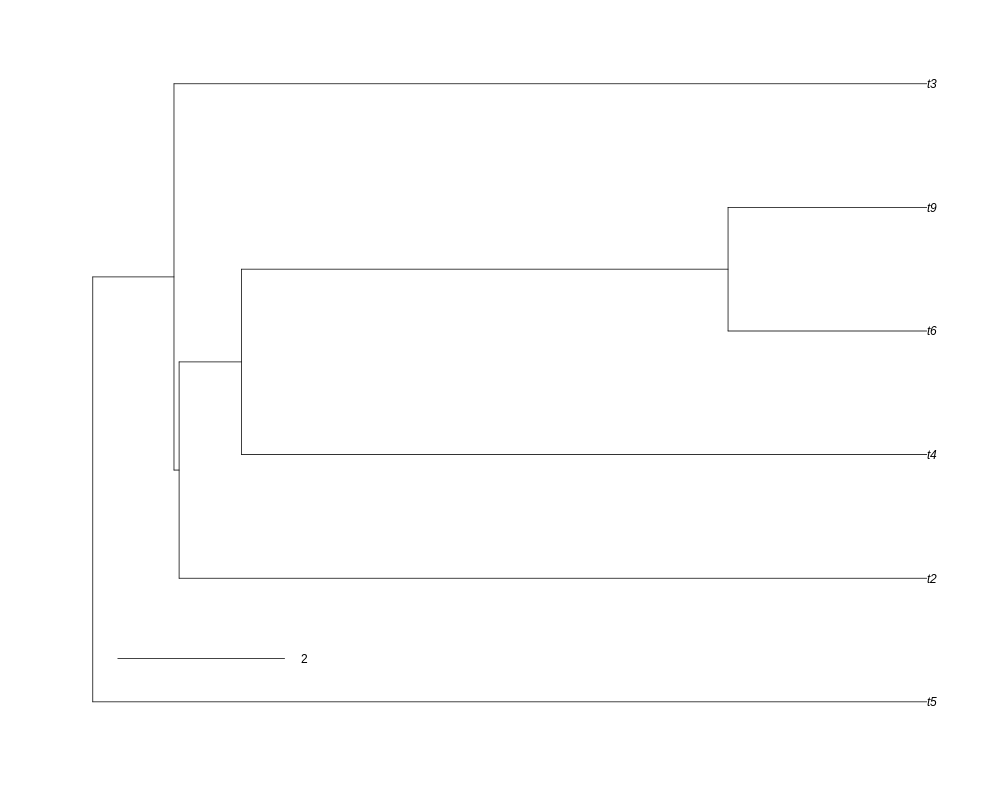
\includegraphics[height=0.4\textheight]{pirouette_example_30/example_30_314/true_tree.png}
    };   
    \node[state] (B) [below of = A, rectangle] {
      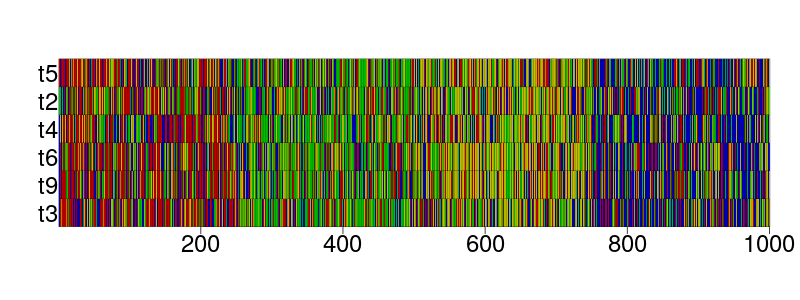
\includegraphics[height=0.25\textheight]{pirouette_example_30/example_30_314/true_alignment.png}
    };   
    \node[state] (CG) [below of = B, rectangle] {
      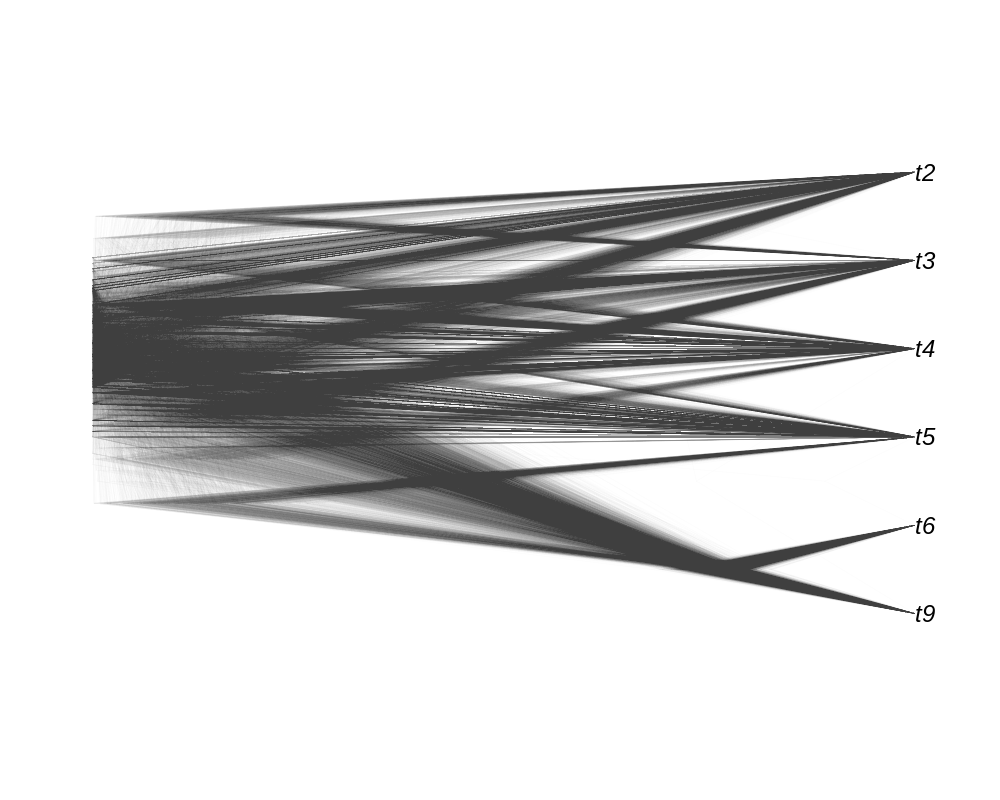
\includegraphics[height=0.3\textheight]{pirouette_example_30/example_30_314/true_posterior_gen.png}
    };   
    \node[state] (DG) [below of = CG, rectangle] {
      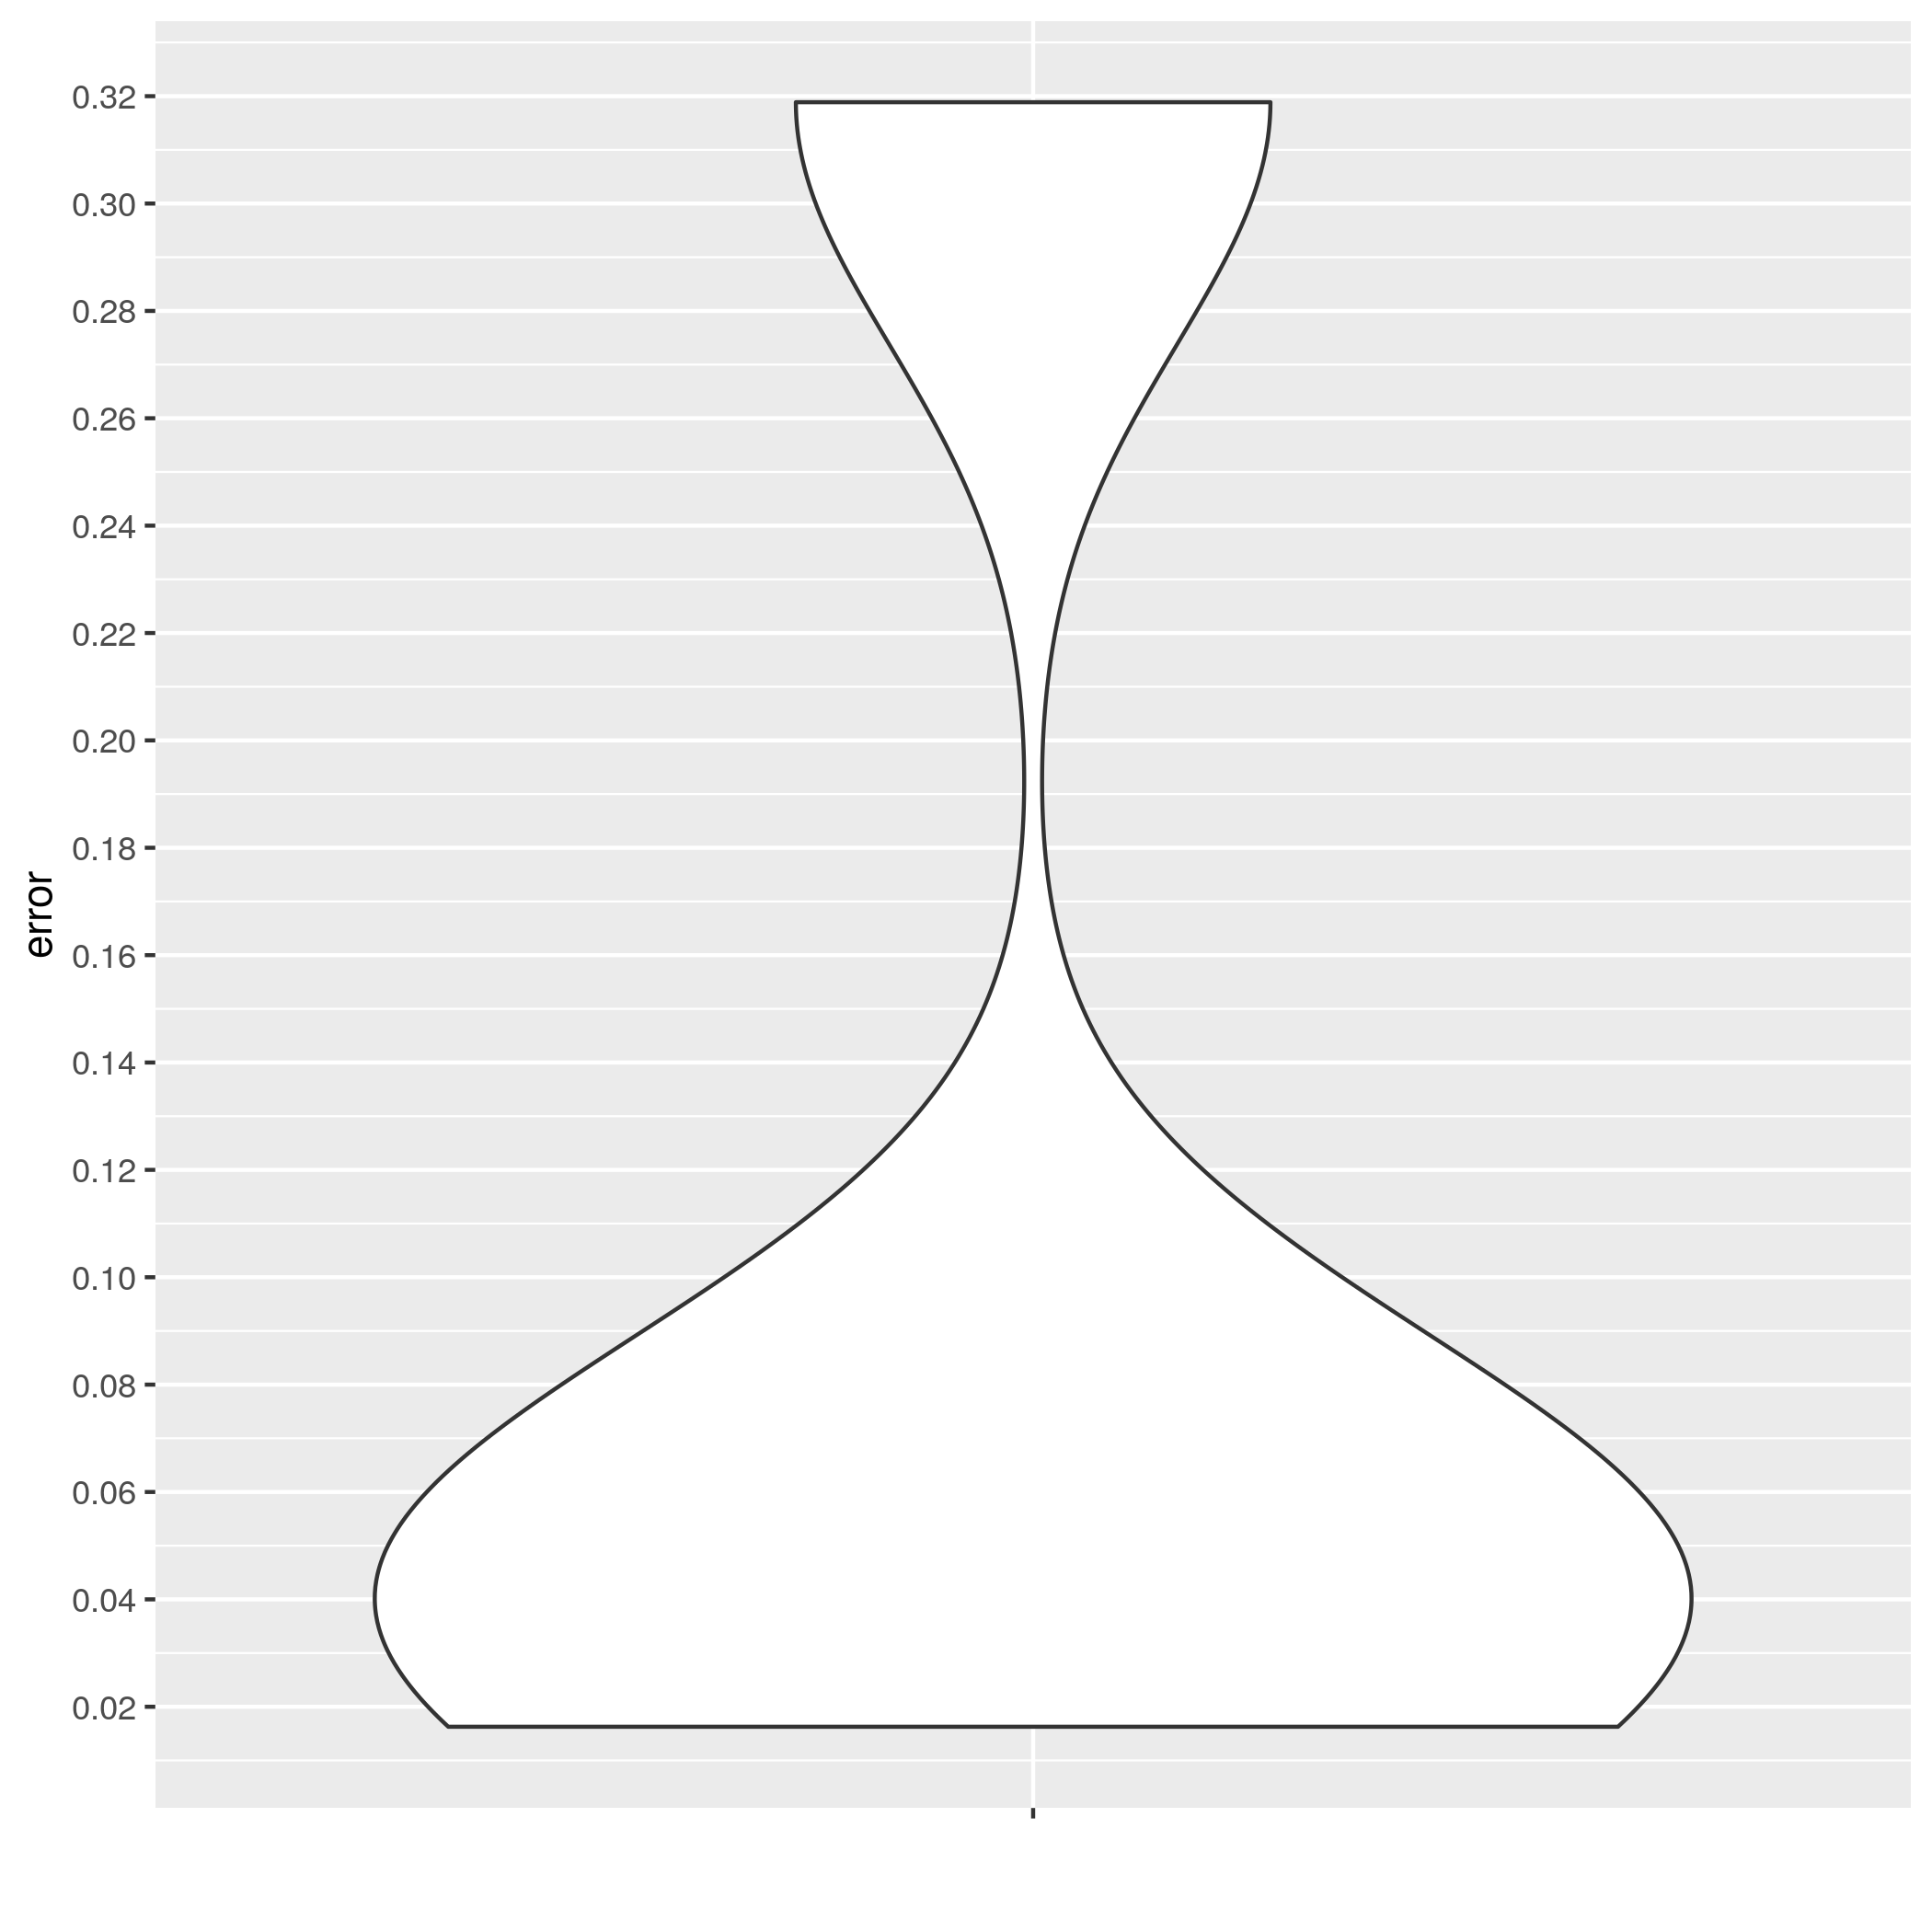
\includegraphics[height=0.3\textheight]{pirouette_example_30/example_30_314/true_error_violin_gen.png}
    };   
    \node[state] (CB) [right of = CG, rectangle] {
      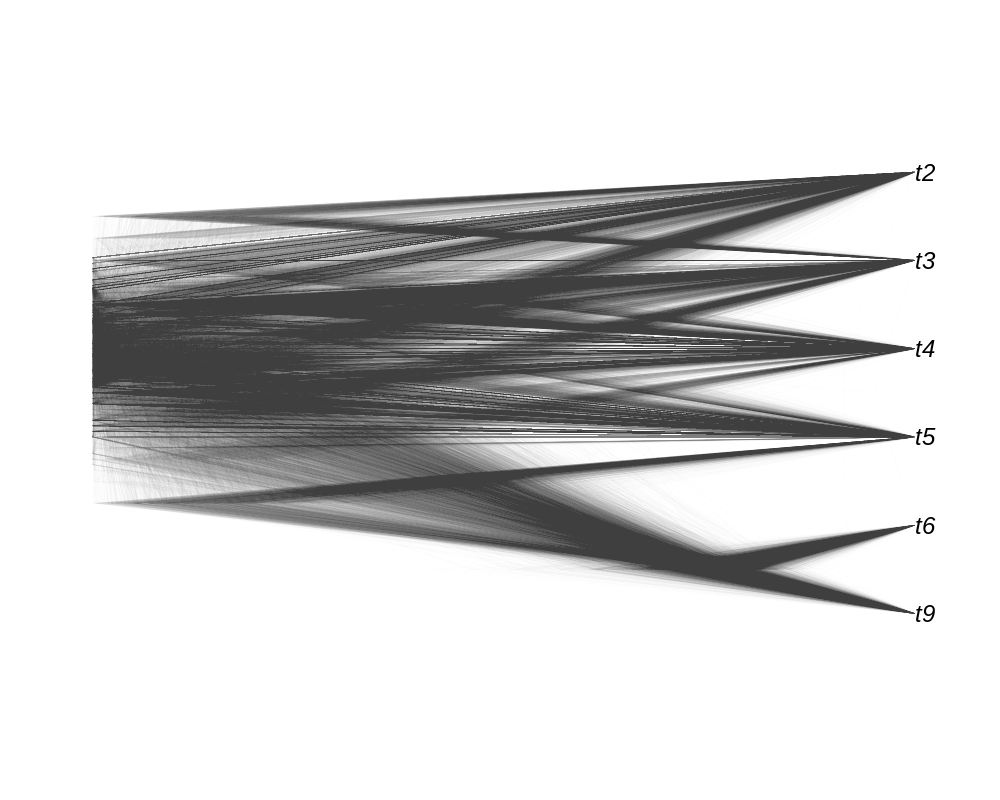
\includegraphics[height=0.3\textheight]{pirouette_example_30/example_30_314/true_posterior_best.png}
    };   
    \node[state] (DB) [below of = CB, rectangle] {
      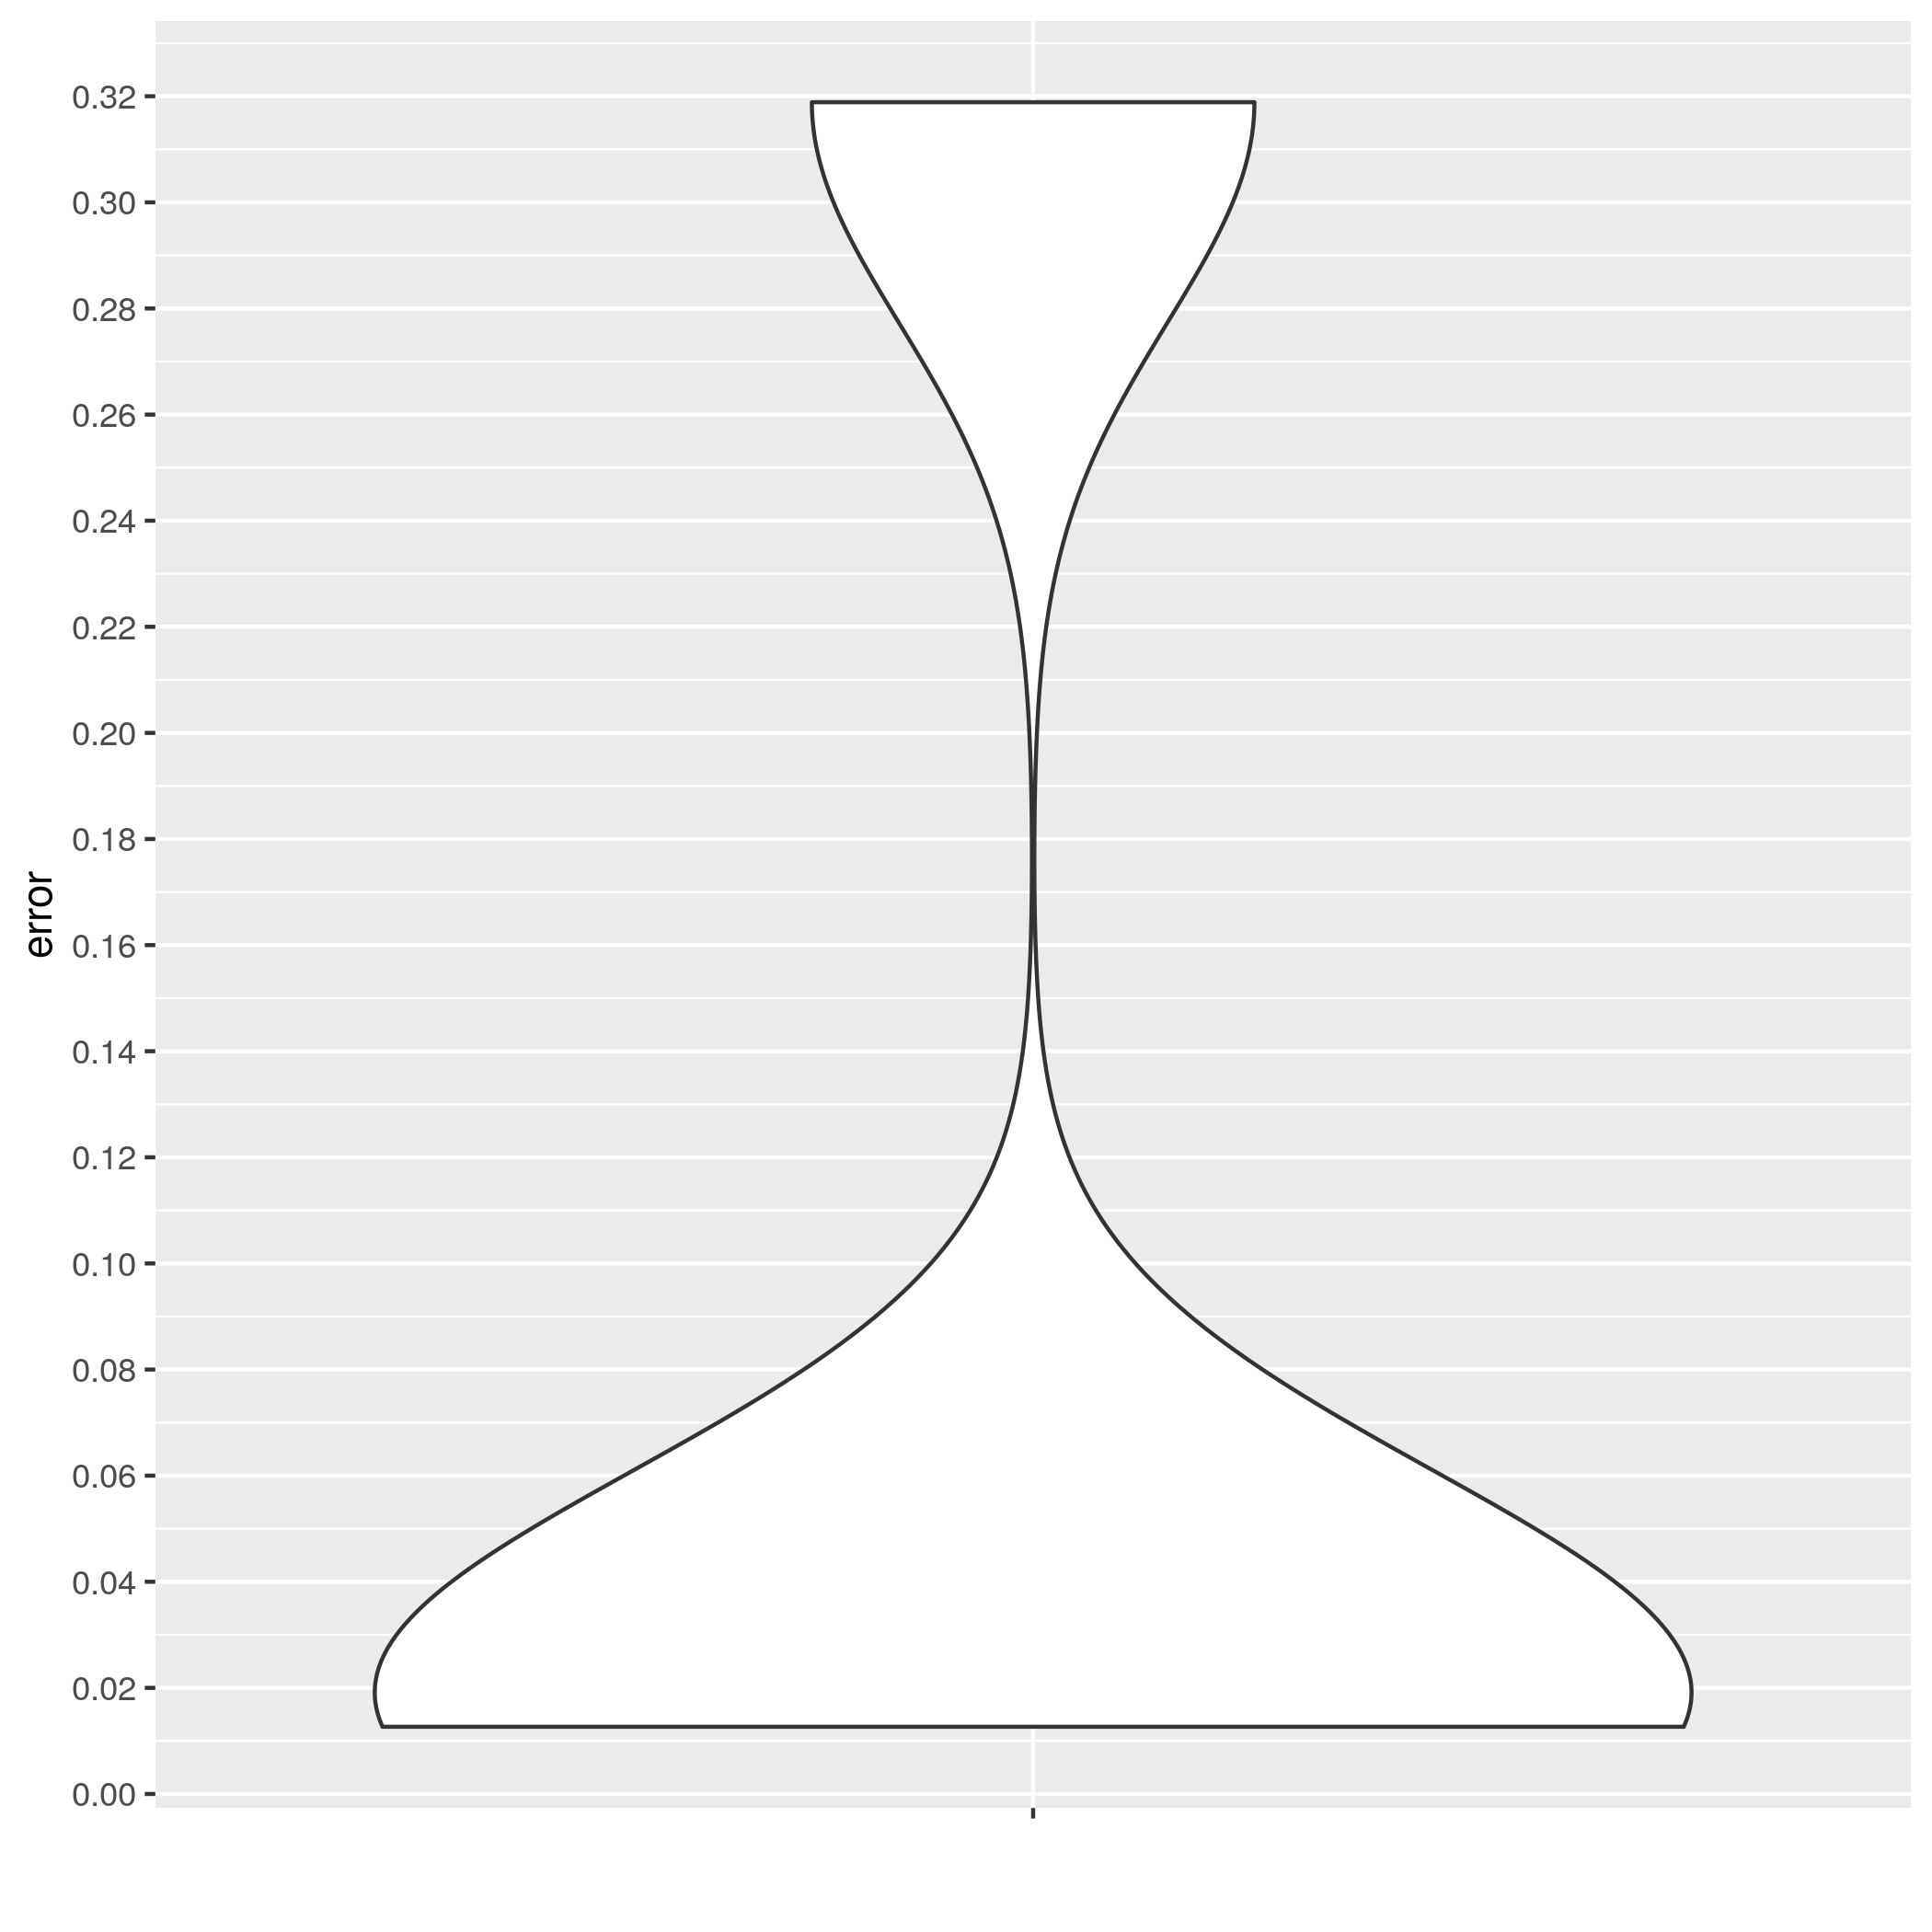
\includegraphics[height=0.3\textheight]{pirouette_example_30/example_30_314/true_error_violin_best.png}
    };   
    \node[state] (AT) [right of = A, rectangle, node distance=0.8\textheight] {
      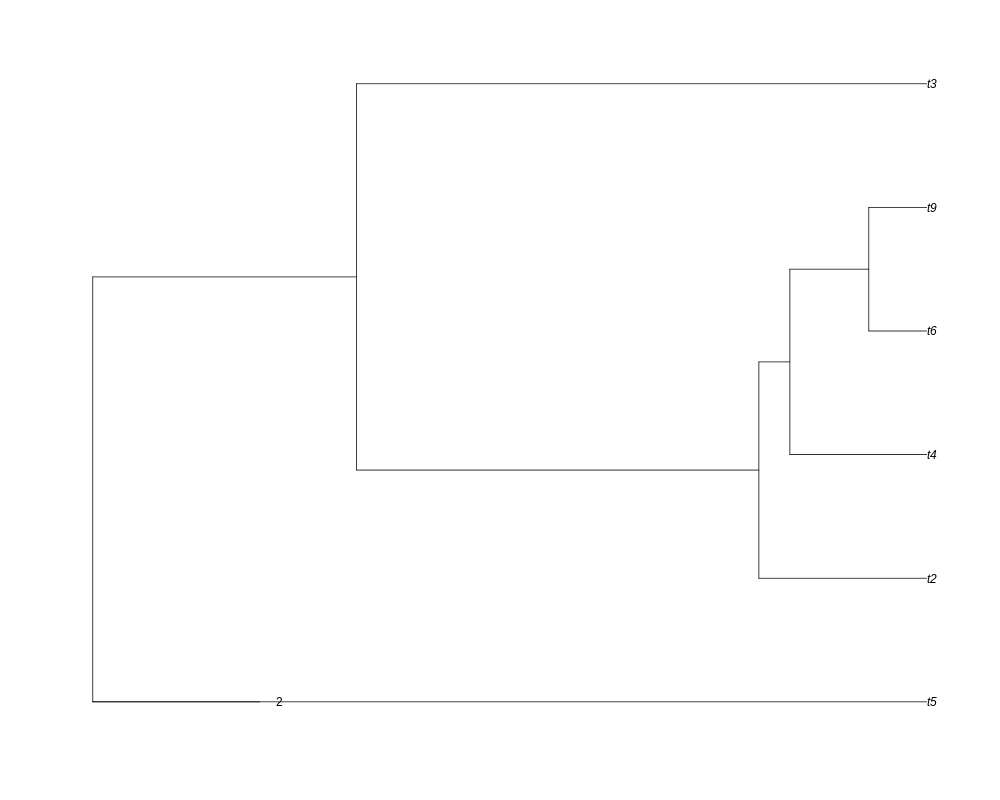
\includegraphics[height=0.4\textheight]{pirouette_example_30/example_30_314/twin_tree.png}
    };   
    \node[state] (BT) [below of = AT, rectangle] {
      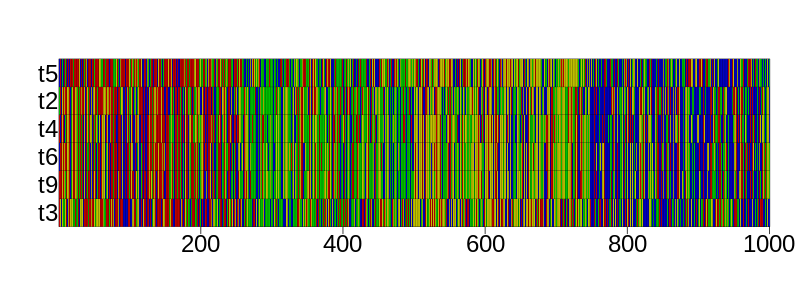
\includegraphics[height=0.25\textheight]{pirouette_example_30/example_30_314/twin_alignment.png}
    };   
    \node[state] (CTG) [right of = CB, rectangle] {
      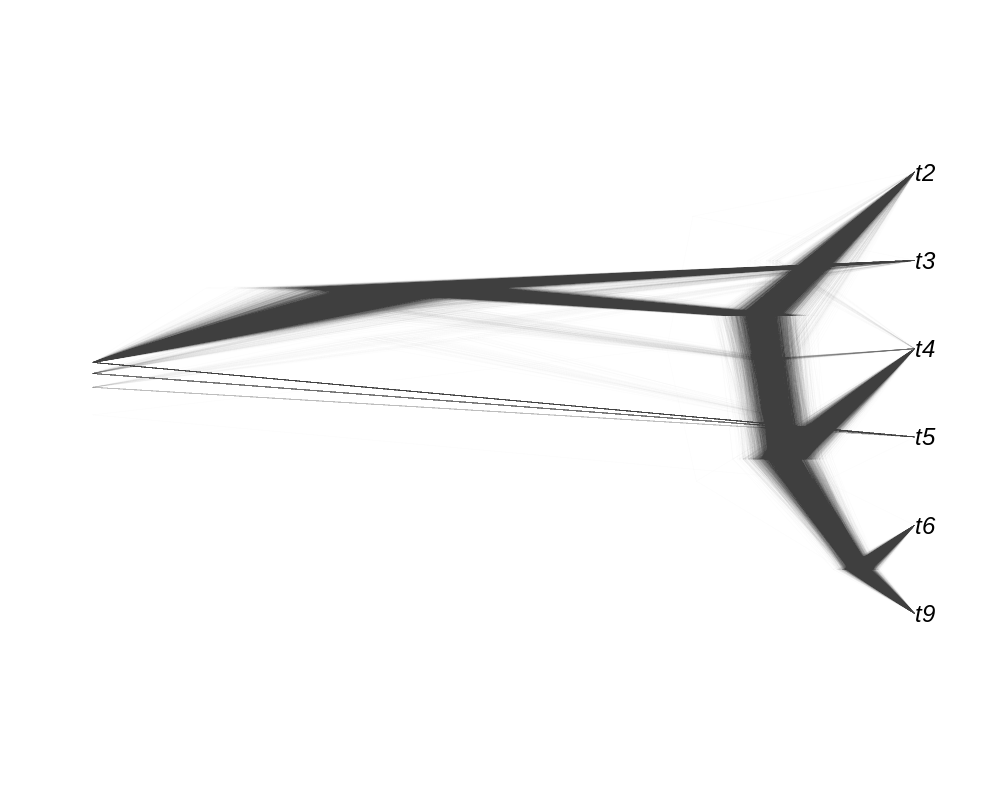
\includegraphics[height=0.3\textheight]{pirouette_example_30/example_30_314/twin_posterior_gen.png}
    };   
    \node[state] (DTG) [below of = CTG, rectangle] {
      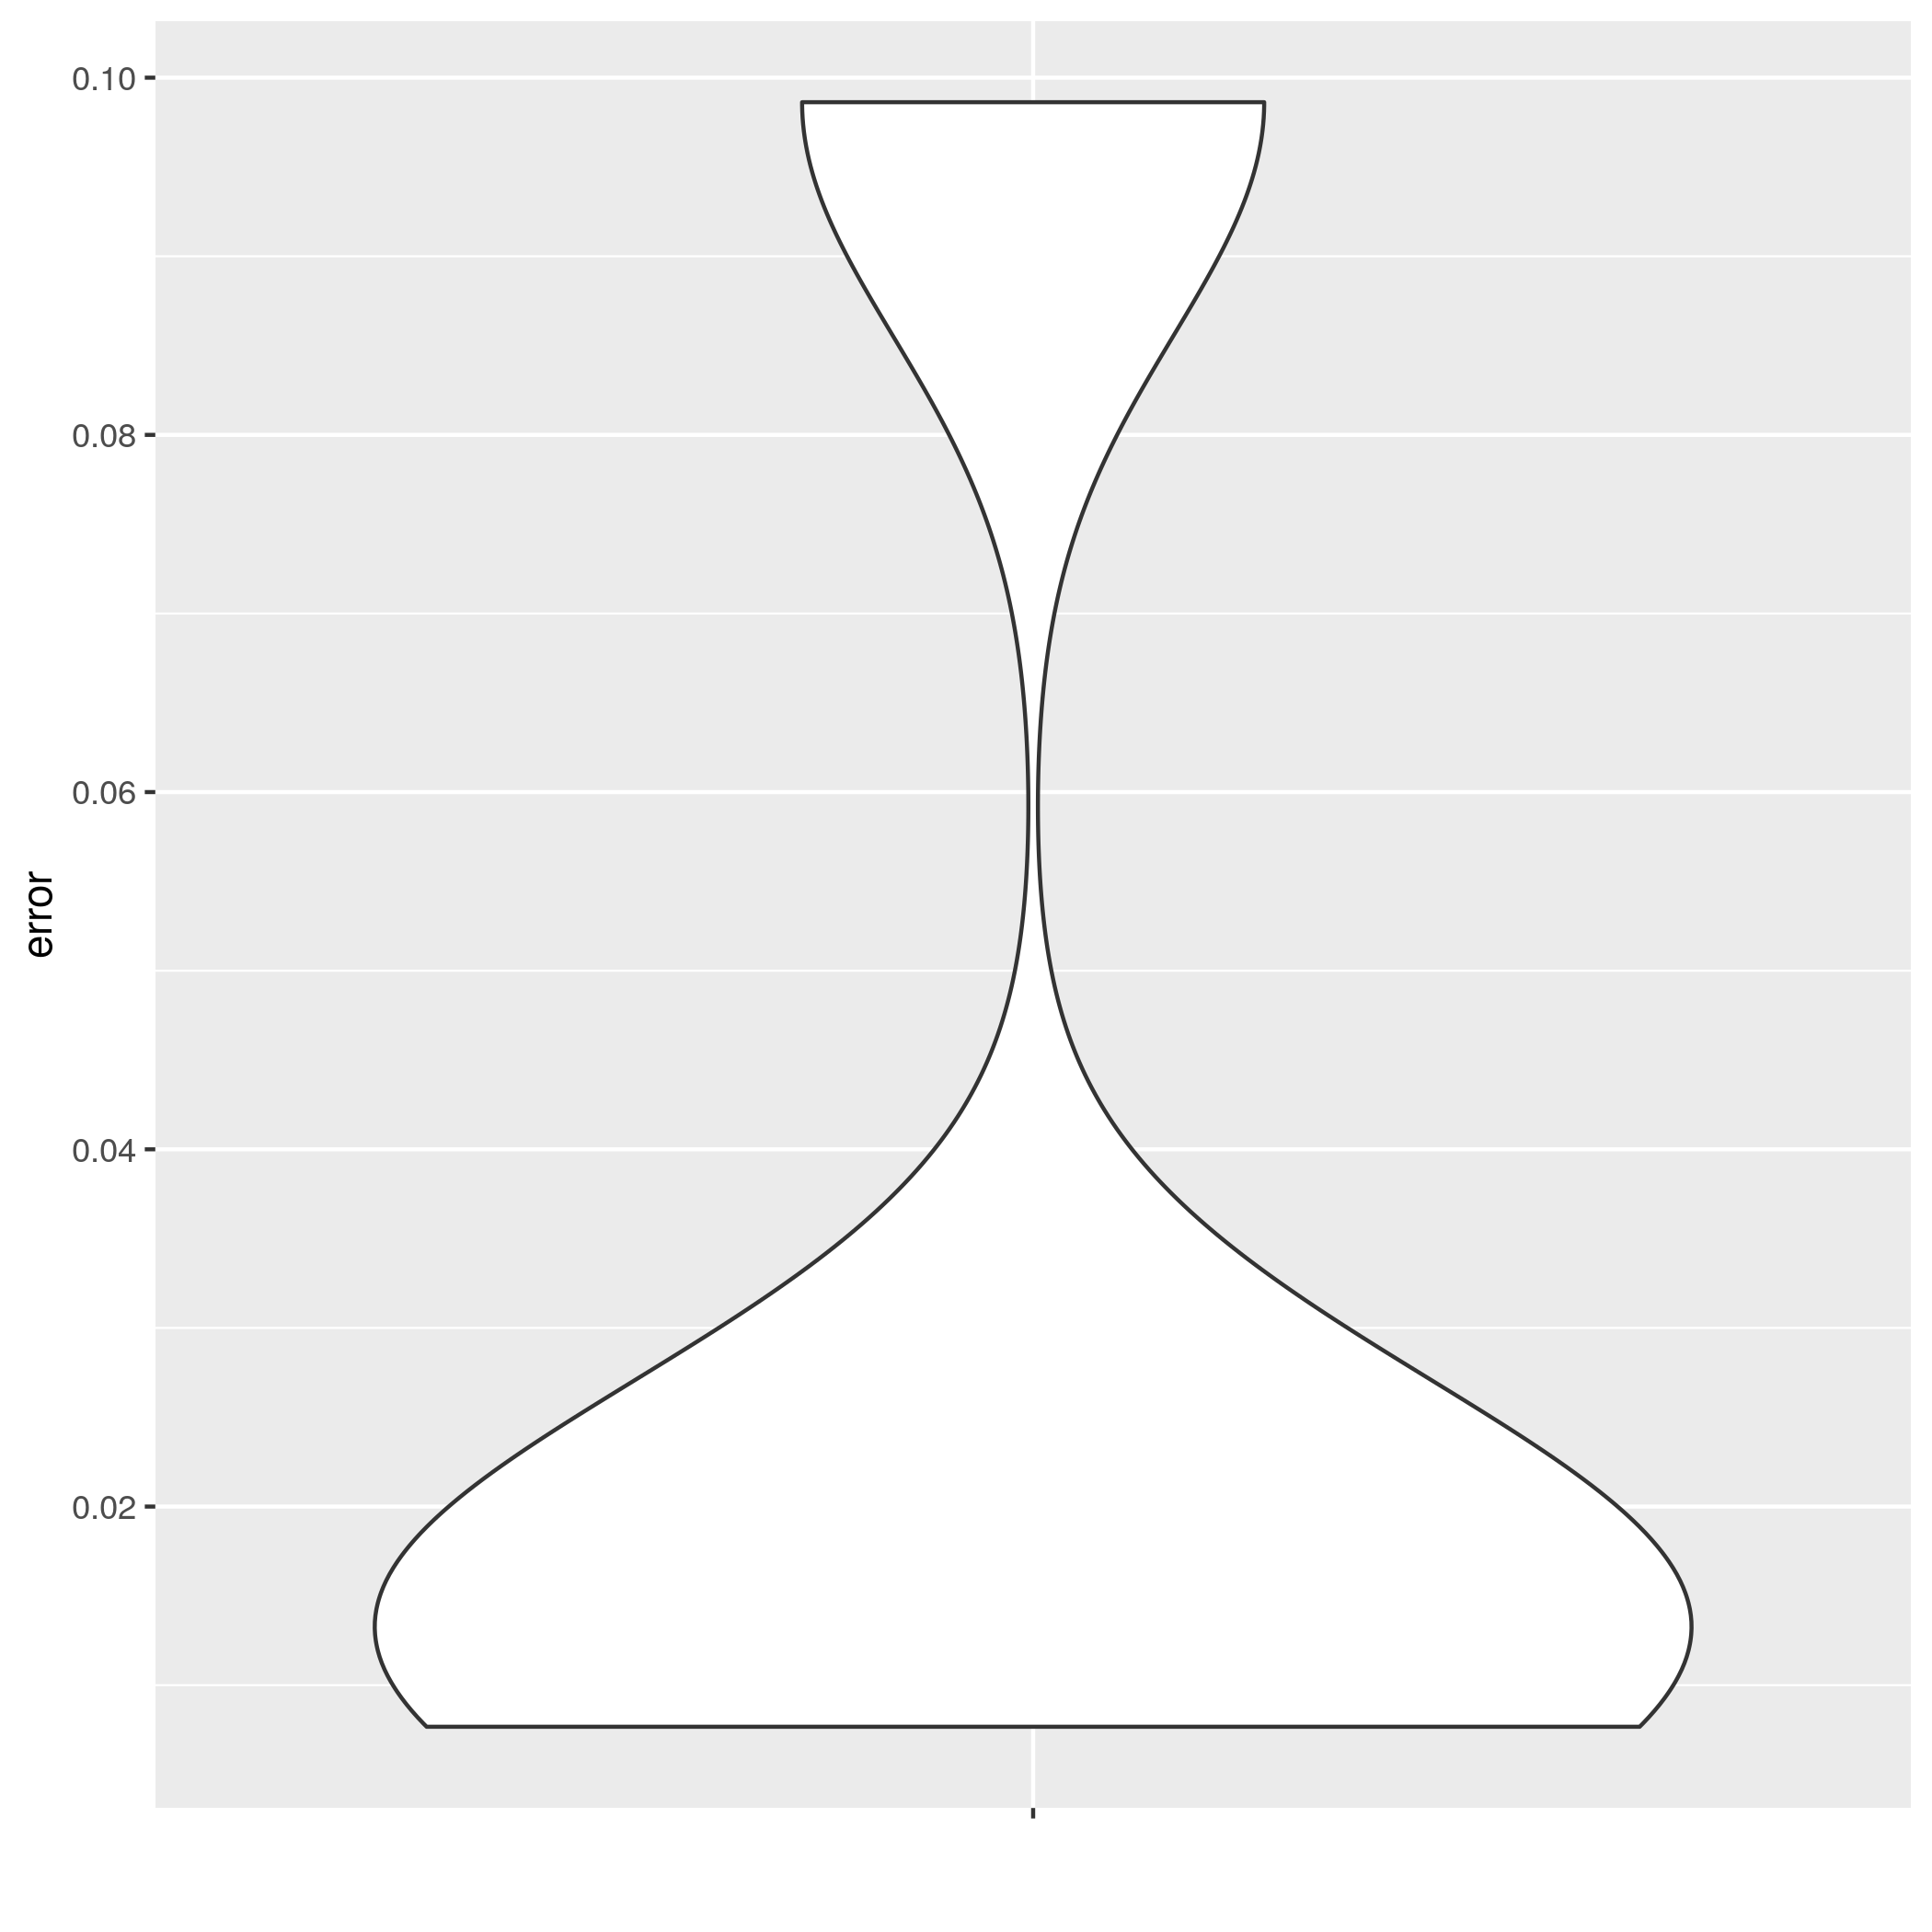
\includegraphics[height=0.3\textheight]{pirouette_example_30/example_30_314/twin_error_violin_gen.png}
    };   
    \node[state] (CTB) [right of = CTG, rectangle] {
      
\includegraphics[height=0.3\textheight]{pirouette_example_30/example_30_314/twin_posterior_best.png}
    };   
    \node[state] (DTB) [below of = CTB, rectangle] {
      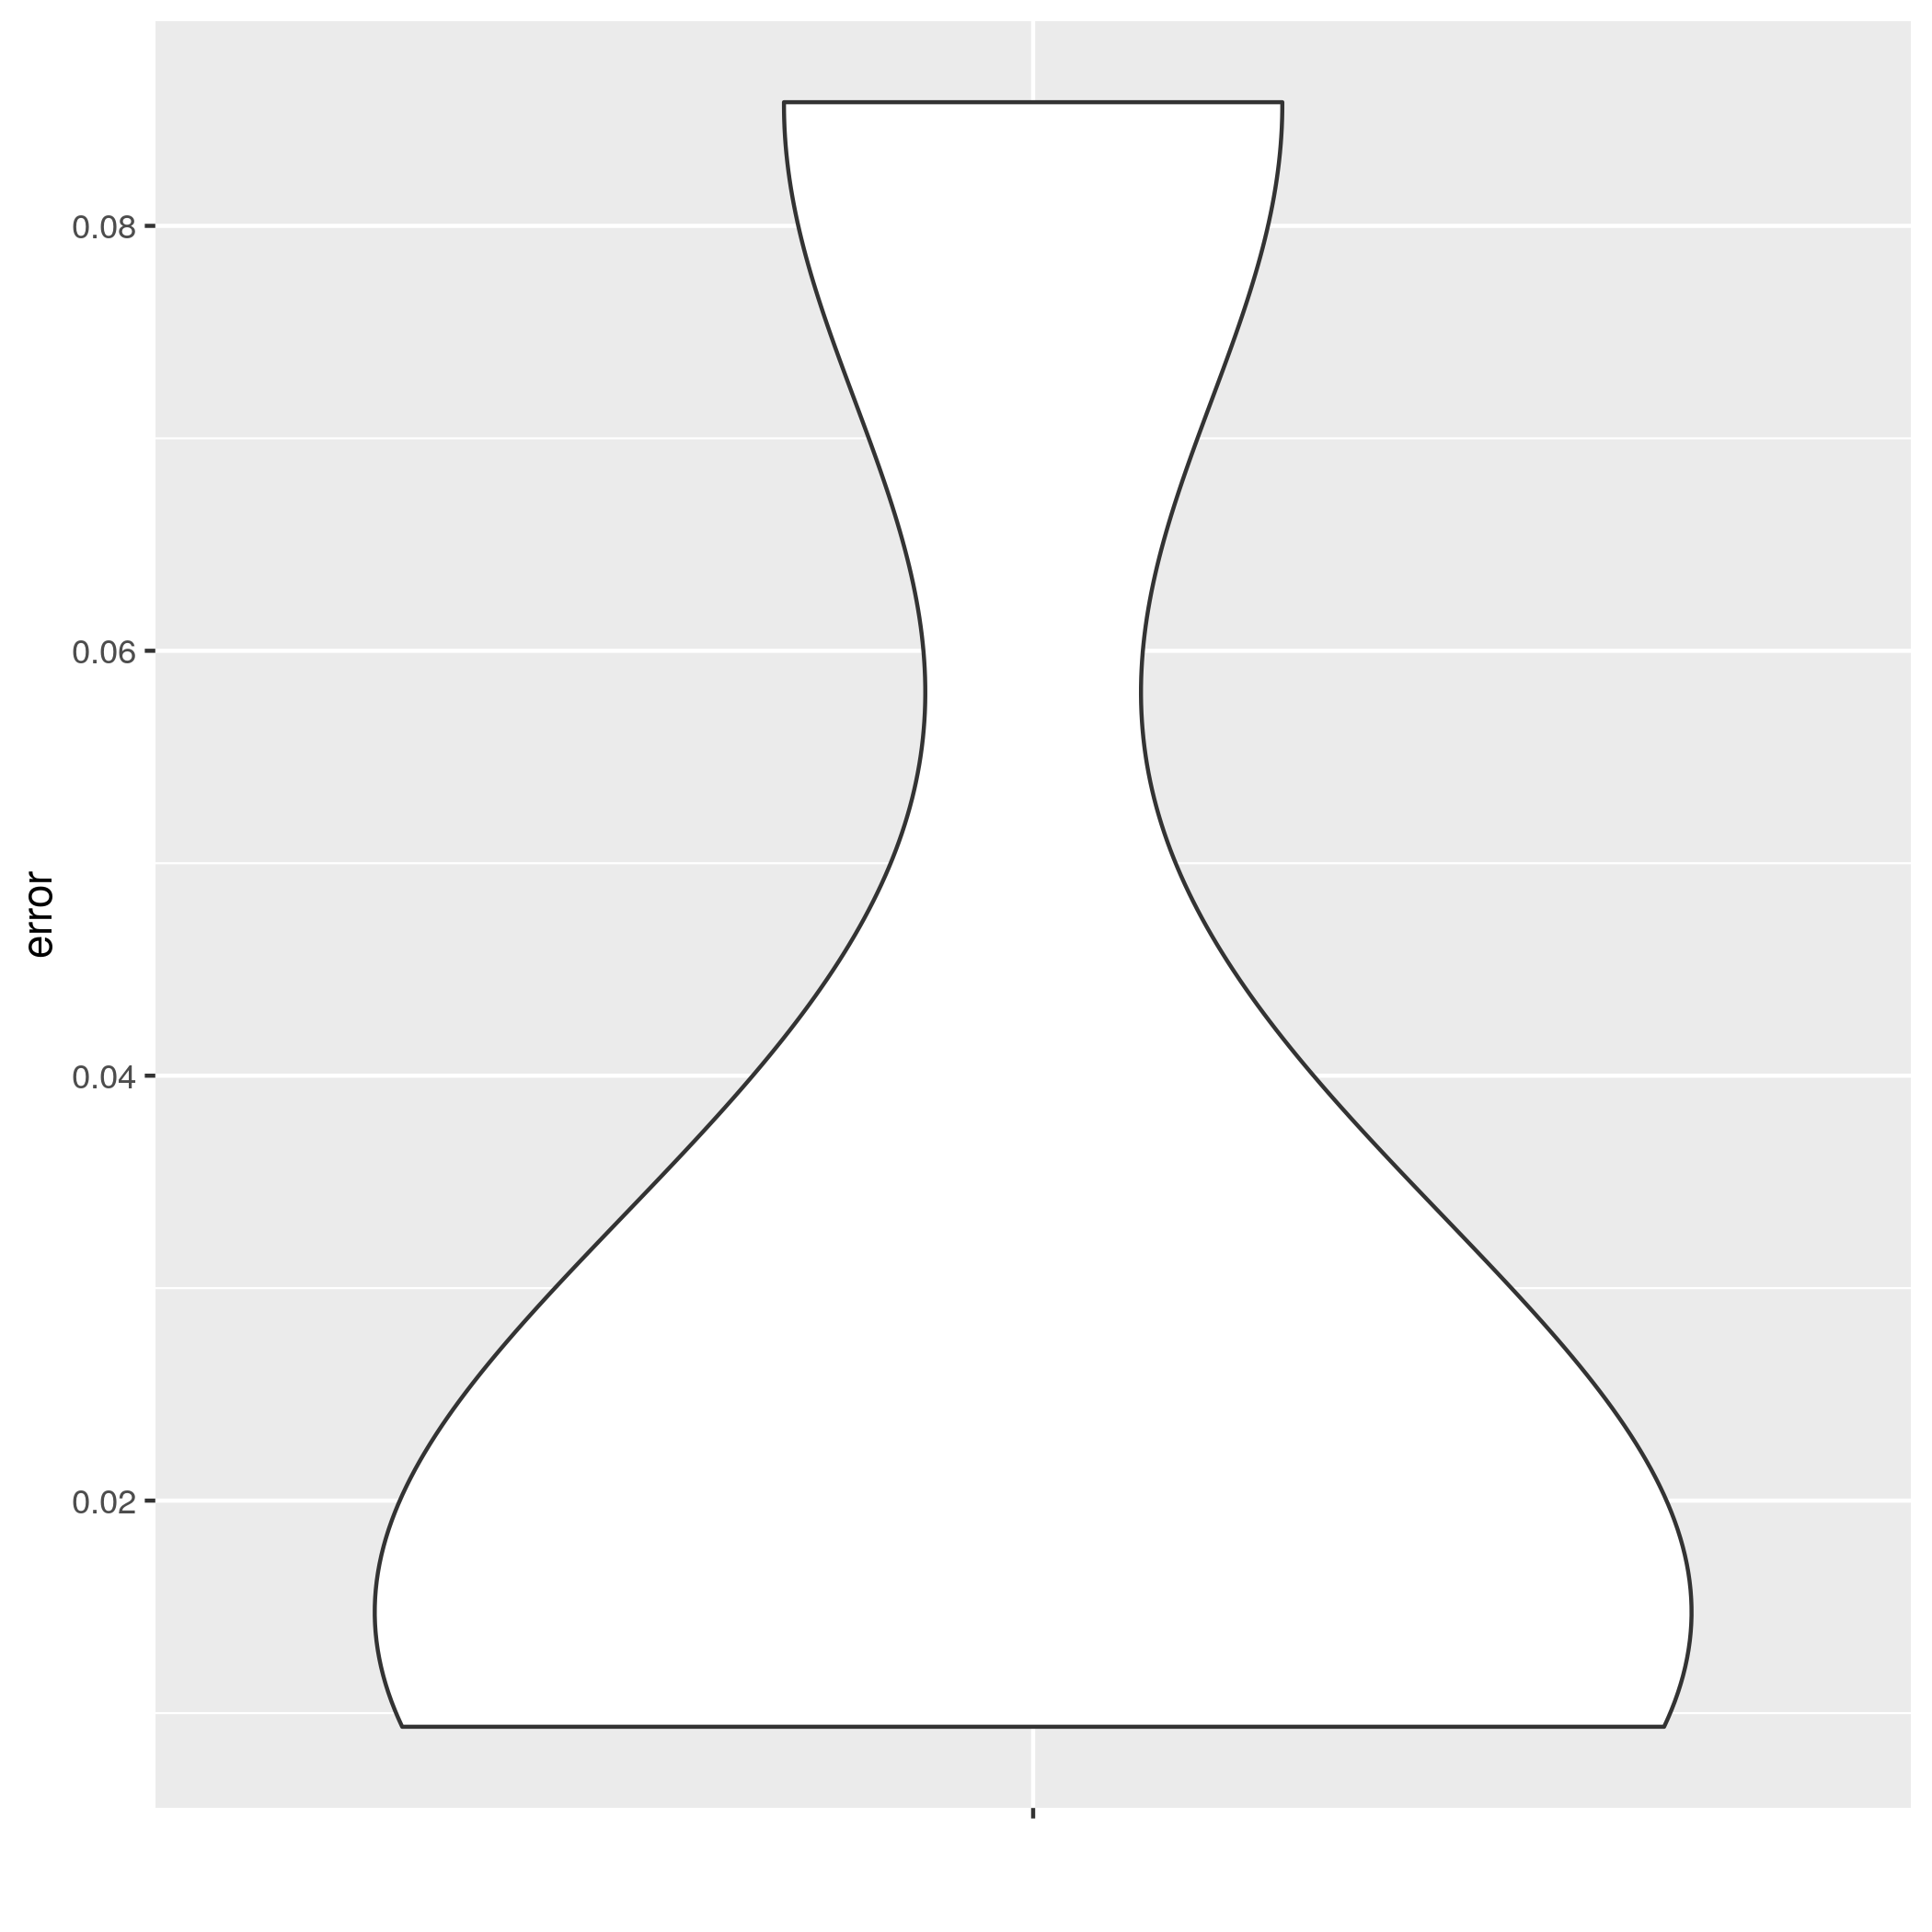
\includegraphics[height=0.3\textheight]{pirouette_example_30/example_30_314/twin_error_violin_best.png}
    };   
    \path 
      (O) edge [anchor = south] node {} (A)
      (A) edge [anchor = south] node {} (B)
      (B) edge [anchor = south] node {} (CG)
      (CG) edge [anchor = south] node {} (DG)
      (B) edge [anchor = south east] node {} (CB)
      (CB) edge [anchor = south] node {} (DB)
      (A) edge [anchor = east] node {} (AT)
      (AT) edge [anchor = south] node {} (BT)
      (BT) edge [anchor = south east] node {} (CTG)
      (CTG) edge [anchor = south] node {} (DTG)
      (BT) edge [anchor = south] node {} (CTB)
      (CTB) edge [anchor = south] node {} (DTB)
    ; 
    \end{tikzpicture}
  }
  \caption{Full pirouette pipeline, including comparison to baseline error. The true tree (top right) is used to simulate an alignment. From this alignment two posterior distributions of trees are created: one using the generative model and another one using the inference model with the highest marginal likelihood. For each distribution of trees, a distribution of errors, measured with the nLTT statistic, between the posterior trees and the main trees is drawn. From the true tree also a twin tree is created (right side of the figure) which follows the same pipeline, leading to two additional error distributions to use as baseline errors.}
  \label{fig:example_30_full_pipeline}
\end{figure}
%%%%%%%%%%%%%%%%%%%%%%%%%%%%%%%%%%%%%%%%%%%%%%%%%%%%%%%%%%%%%%%%%%%%%%%%%%%%%%%%

\input{pirouette_example_30/example_30_314/esses_gen.latex}

\input{pirouette_example_30/example_30_314/esses_best.latex}

\input{pirouette_example_30/example_30_314/esses_twin_gen.latex}

\input{pirouette_example_30/example_30_314/esses_twin_best.latex}

\input{pirouette_example_30/example_30_314/evidence_true.latex}

\input{pirouette_example_30/example_30_314/evidence_twin.latex}

\clearpage
%\newpage

%%%%%%%%%%%%%%%%%%%%%%%%%%%%%%%%%%%%%%%%%%%%%%%%%%%%%%%%%%%%%%%%%%%%%%%%%%%%%%%%
\subsection{Using a distribution of trees}
\label{subsec:distribution}
%%%%%%%%%%%%%%%%%%%%%%%%%%%%%%%%%%%%%%%%%%%%%%%%%%%%%%%%%%%%%%%%%%%%%%%%%%%%%%%%

This subsection extends the main example, by using multiple (instead of
one) trees. These trees are produced by running a DD tree simulation
with the same parameters as the main example.

The code to reproduce this figure can be found at  
\url{https://github.com/richelbilderbeek/pirouette_example_28}.

\begin{figure}[H]
  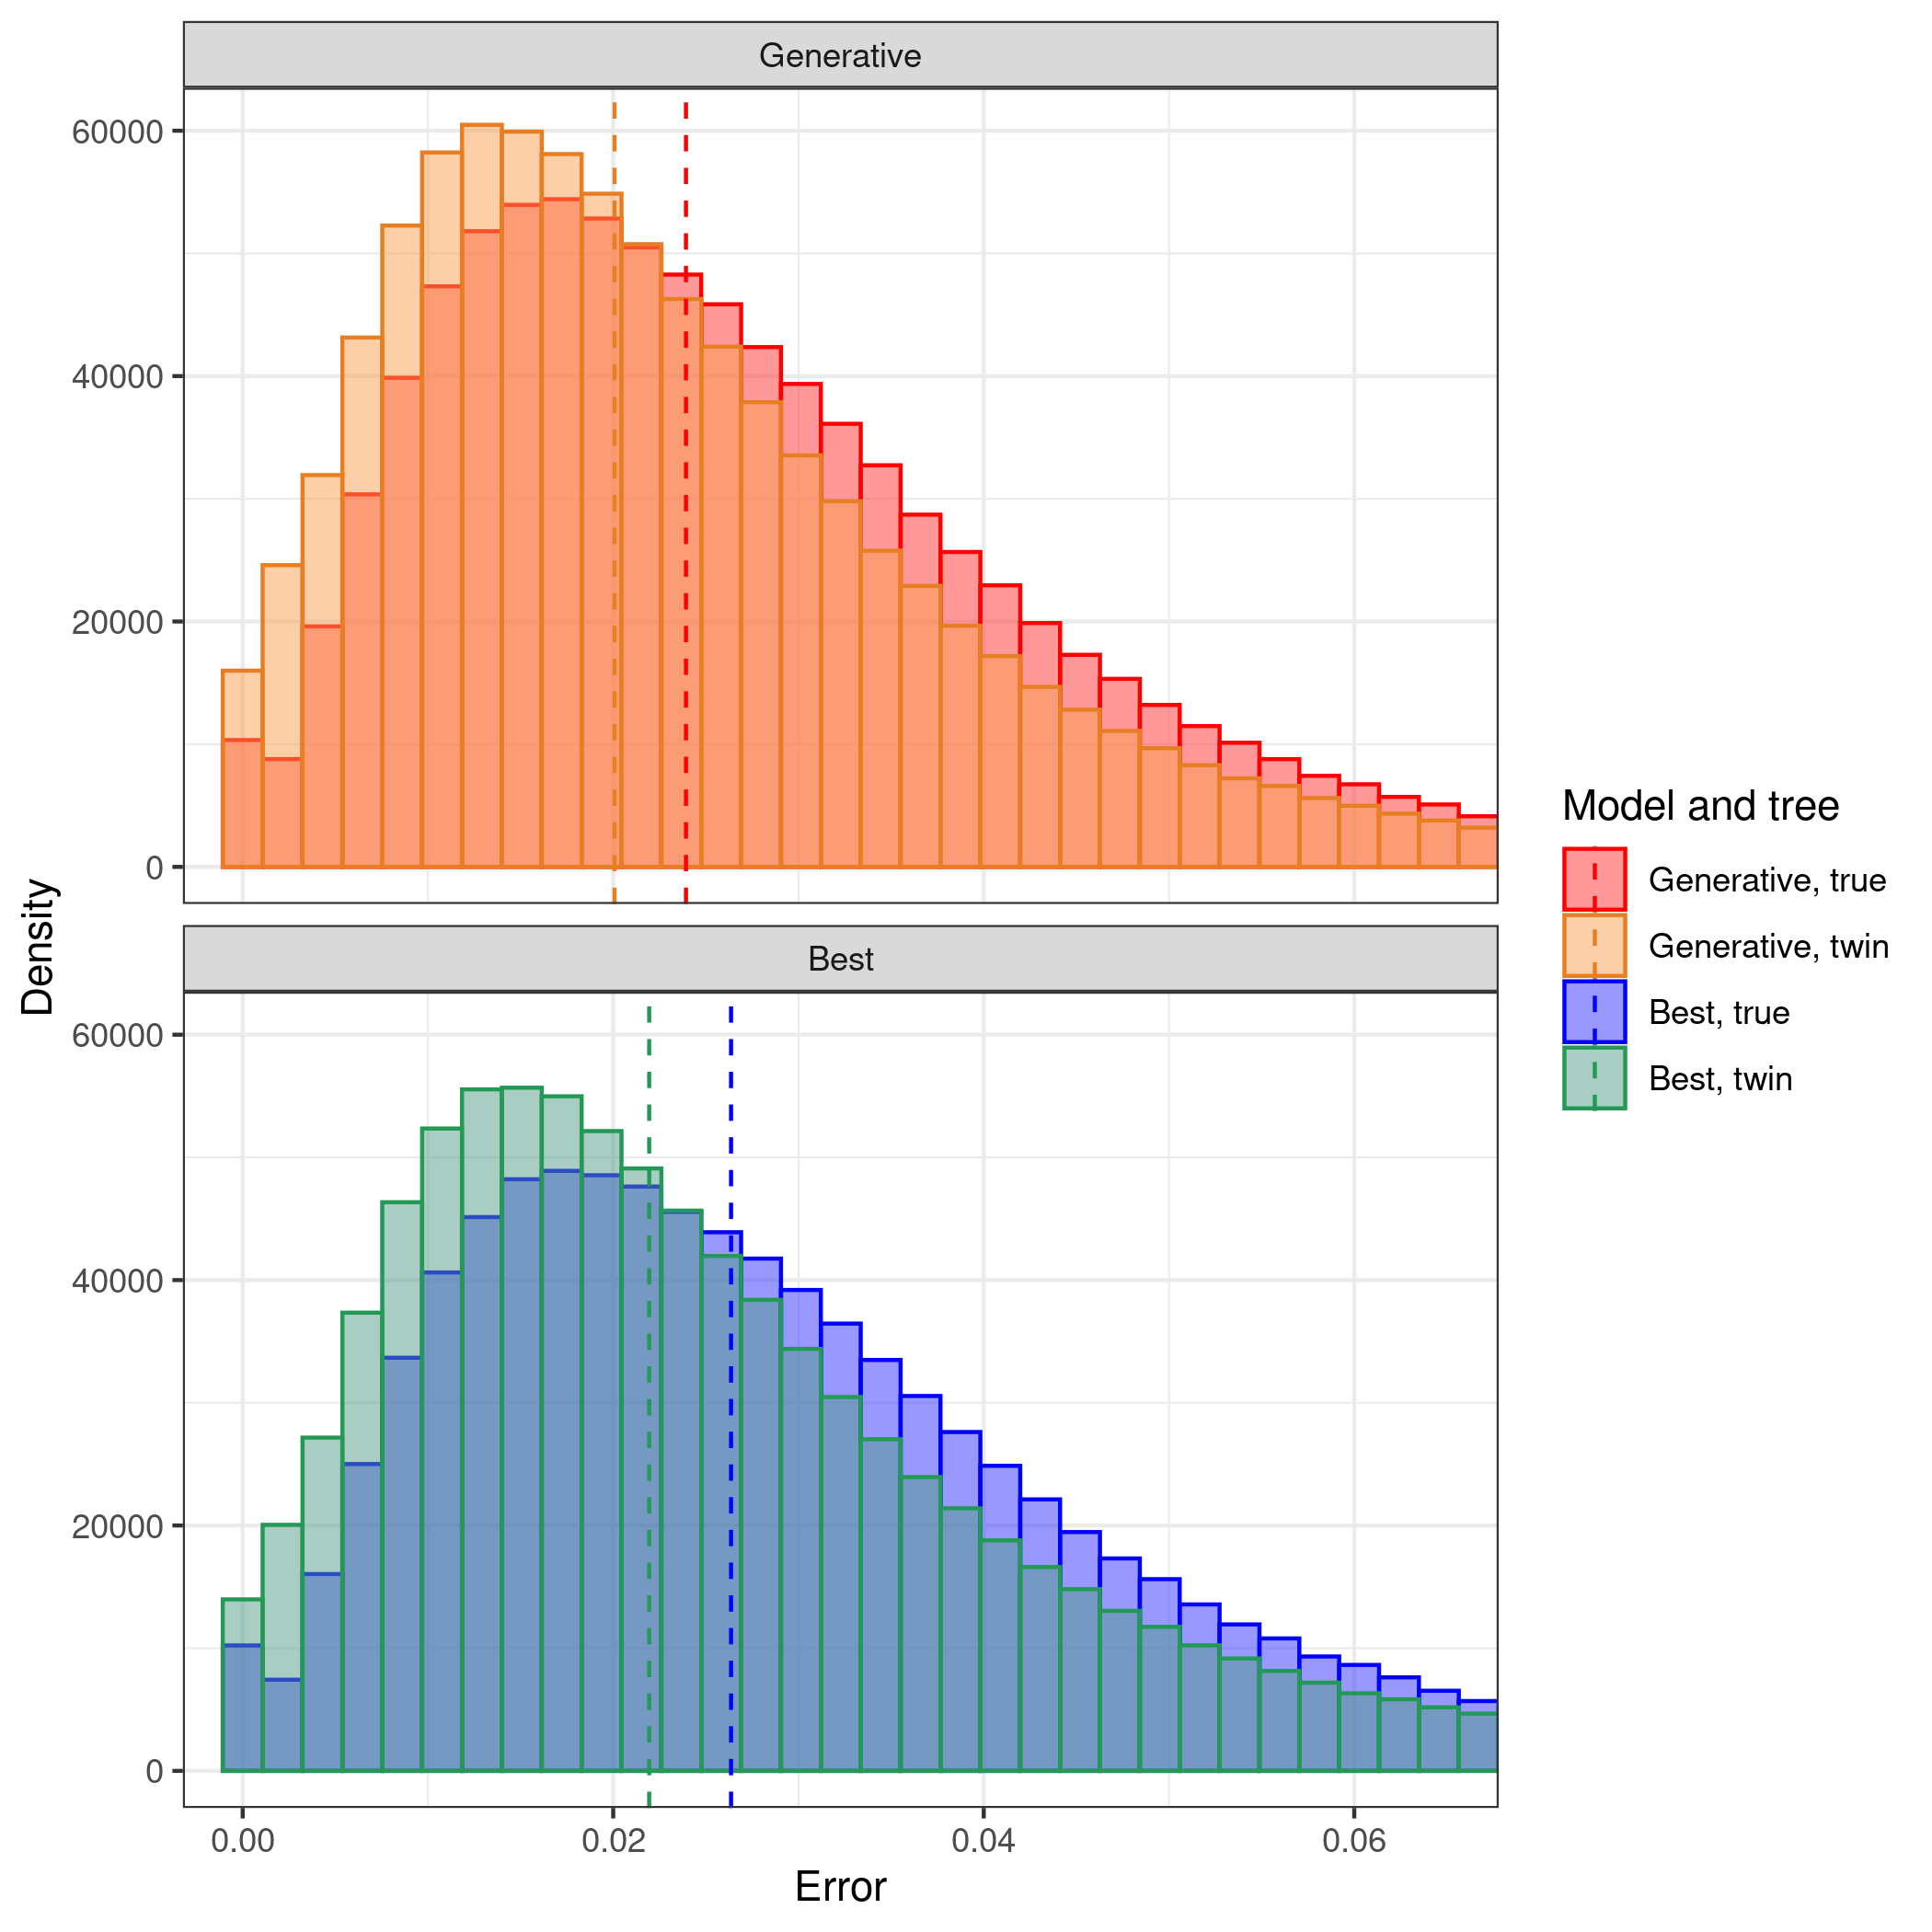
\includegraphics[width=\textwidth]{pirouette_example_28/errors.png}
  \caption{Aggregate error distributions, similar to Fig. \ref{fig:example_30} for the main example, but now for a collection of 20 replicate trees. For each setting (true generative, true best candidate, twin generative and twin best candidate), the resulting errors from each replicate pipeline have been merged into a single distribution.}
  \label{fig:replicate_trees}
\end{figure}

\newpage

%%%%%%%%%%%%%%%%%%%%%%%%%%%%%%%%%%%%%%%%%%%%%%%%%%%%%%%%%%%%%%%%%%%%%%%%%%%%%%%%
\subsection{The effect of the number of taxa}
\label{subsec:n_taxa}
%%%%%%%%%%%%%%%%%%%%%%%%%%%%%%%%%%%%%%%%%%%%%%%%%%%%%%%%%%%%%%%%%%%%%%%%%%%%%%%%

The main example uses 6 taxa. Here we show the same results as the main example,
except for a varying number of taxa. We did so, by setting the DD model's
carrying capacity to the desired number of taxa.

The code to reproduce these figure can be found at  
\url{https://github.com/richelbilderbeek/pirouette_example_28} (6 taxa, main example),
\url{https://github.com/richelbilderbeek/pirouette_example_32} (12 taxa),
\url{https://github.com/richelbilderbeek/pirouette_example_33} (24 taxa),
\url{https://github.com/richelbilderbeek/pirouette_example_41} (32 taxa),
\url{https://github.com/richelbilderbeek/pirouette_example_42} (40 taxa). 

\begin{figure}[H]
  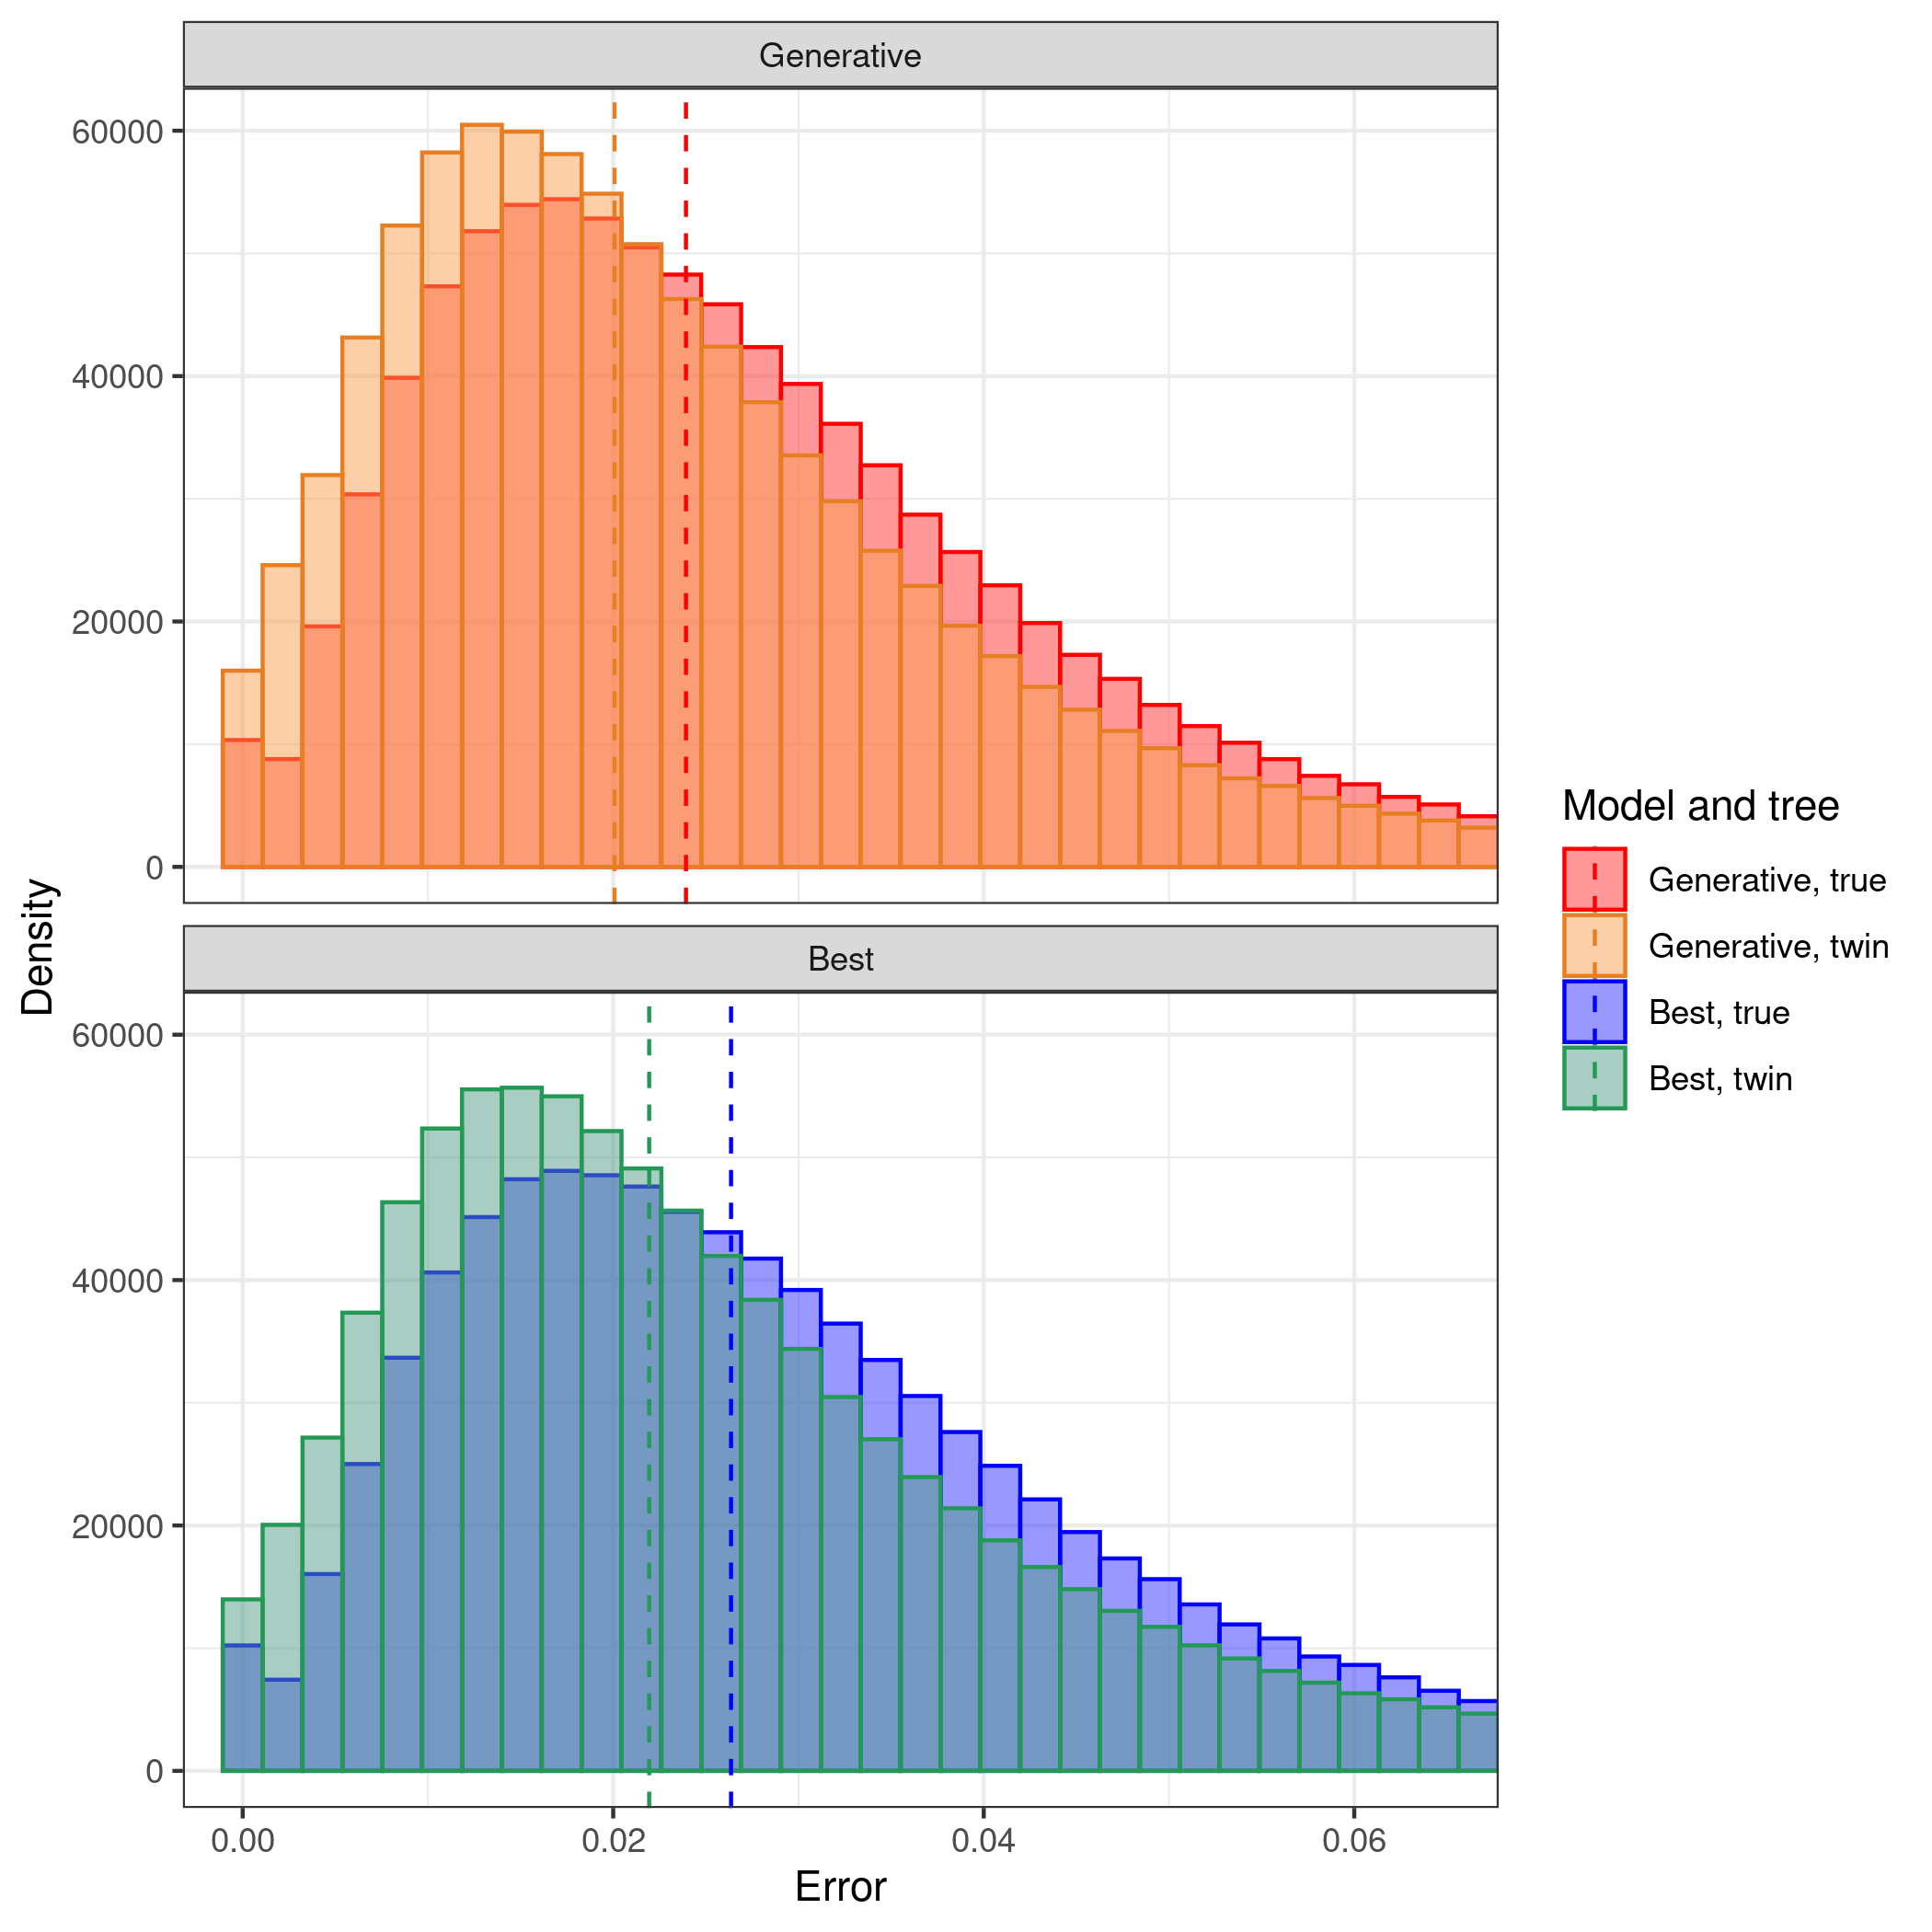
\includegraphics[width=\textwidth]{pirouette_example_28/errors.png}
  \caption{Aggregate error distributions for 20 replicates. Here each true tree has 6 taxa. This took 16 hours to compute.}
\end{figure}

\begin{figure}[H]
  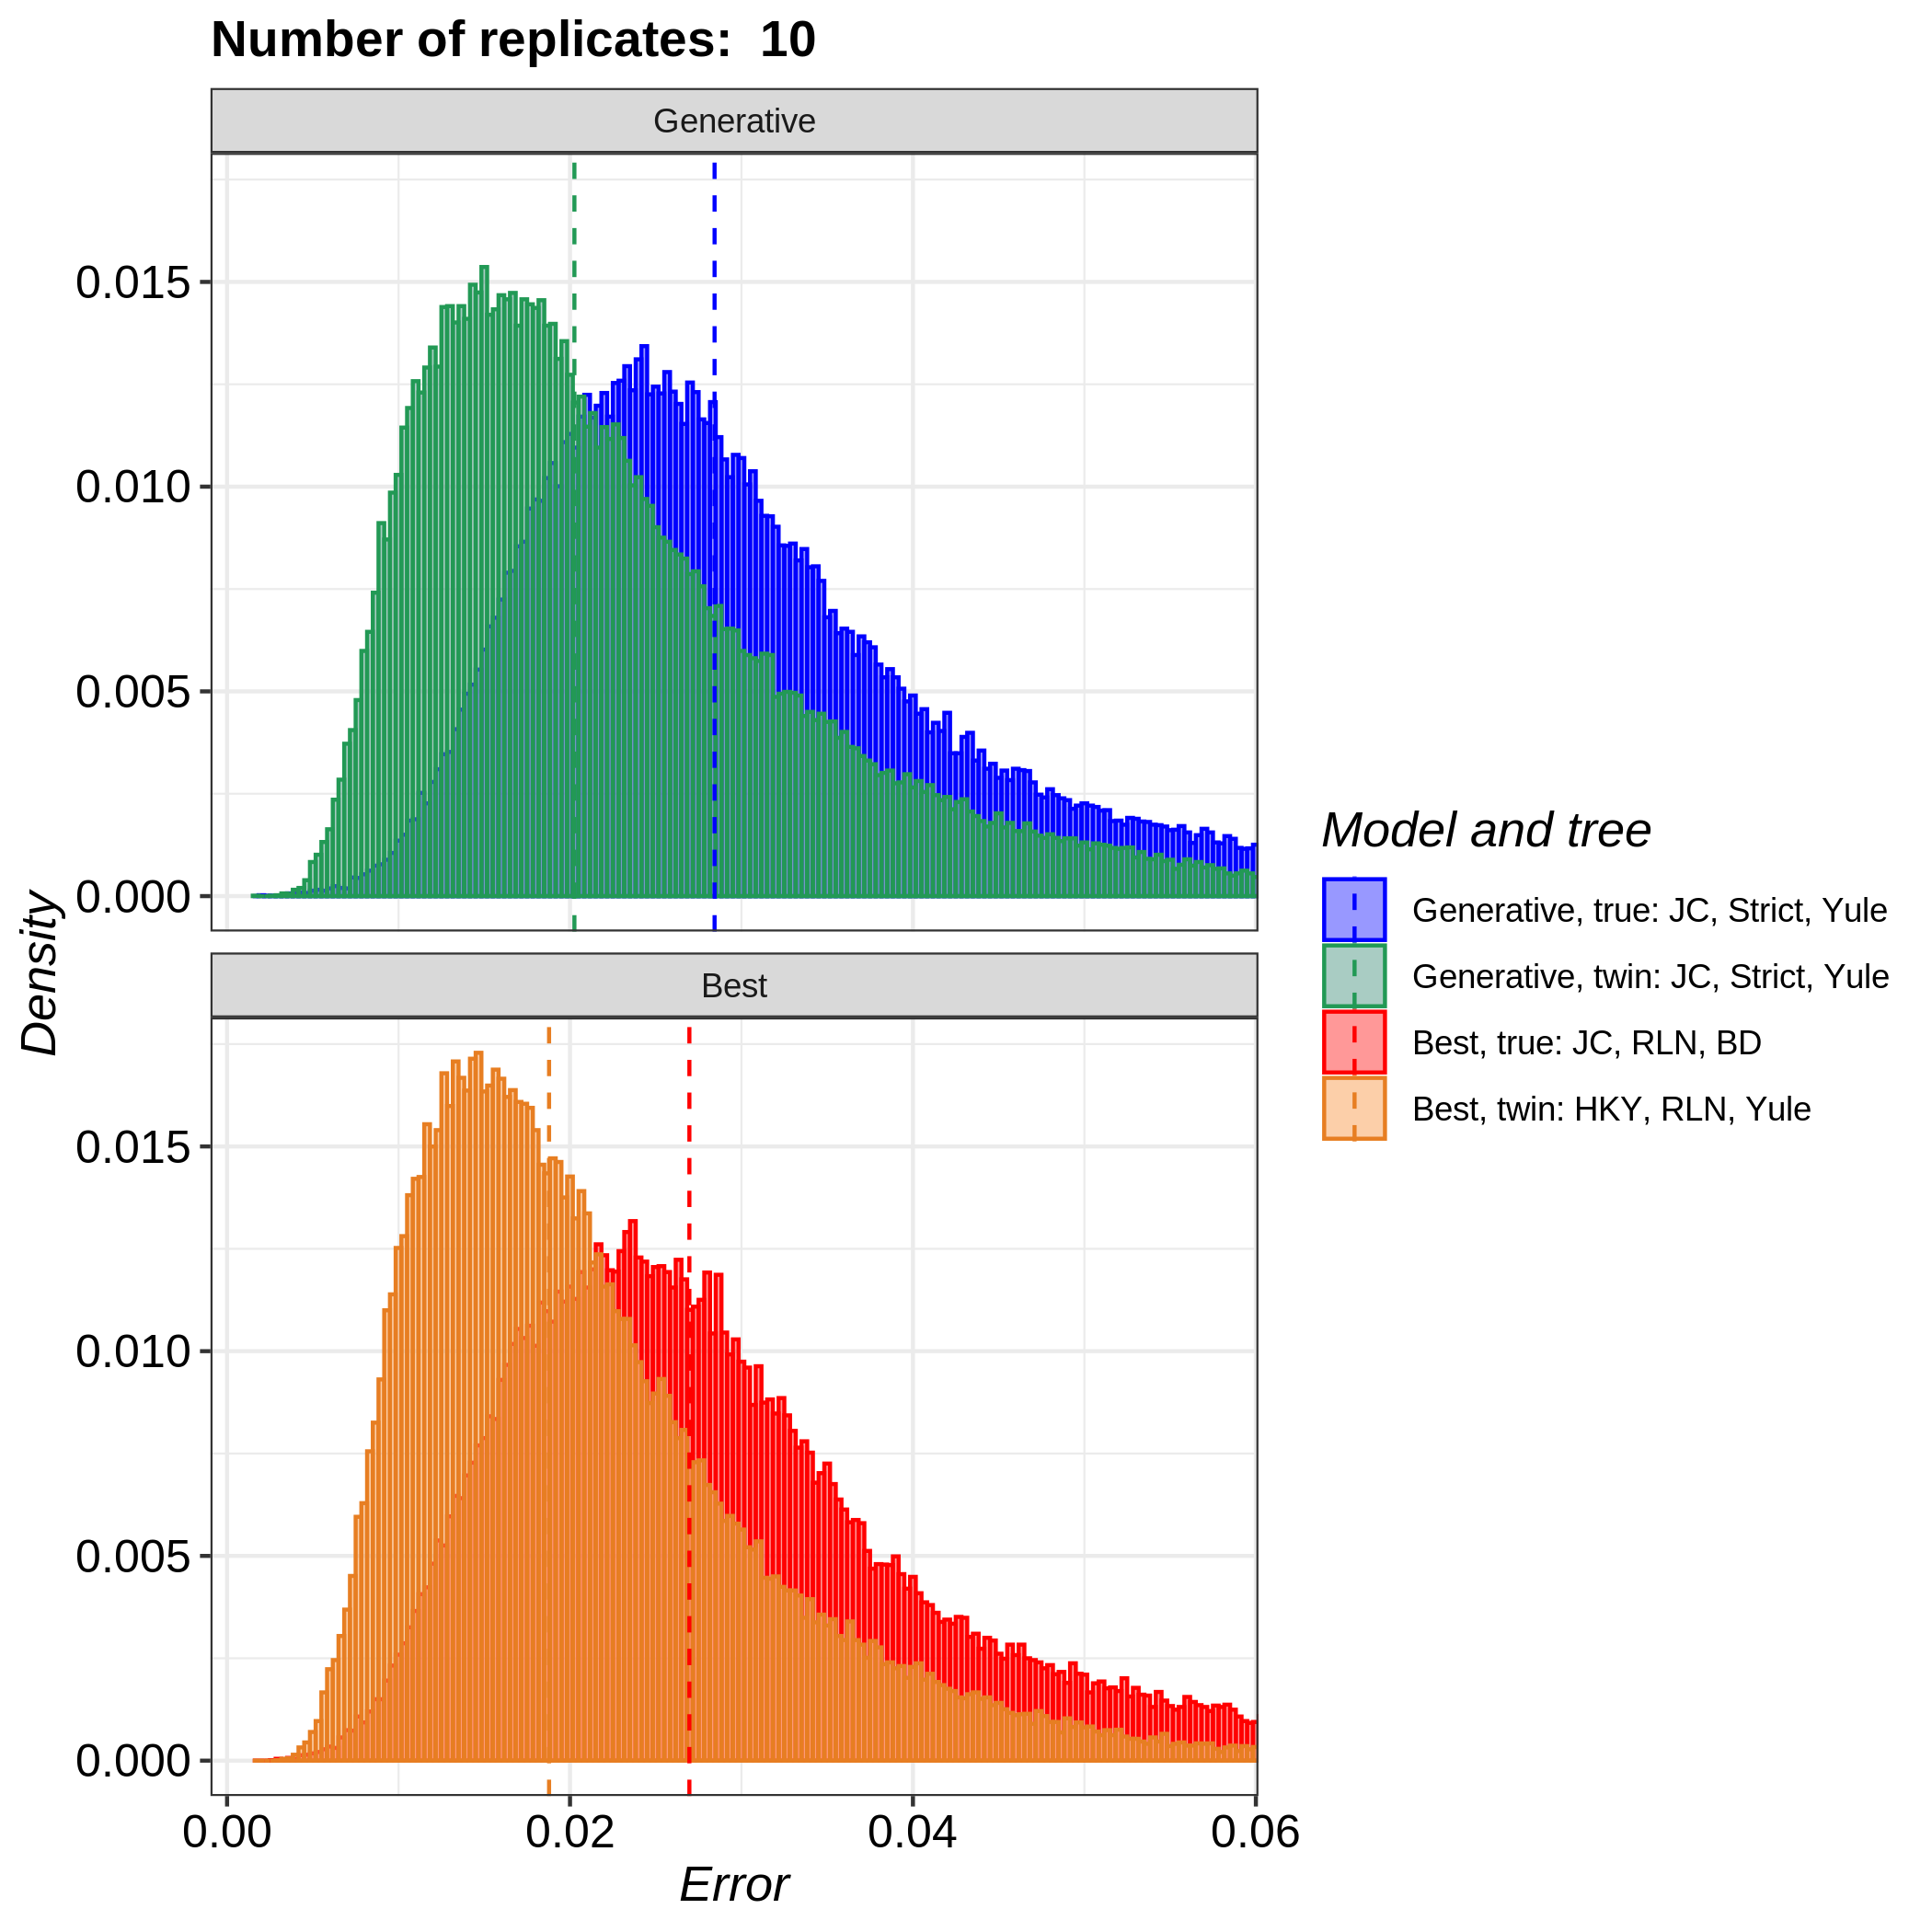
\includegraphics[width=\textwidth]{pirouette_example_32/errors.png}
  \caption{Aggregate error distributions for 10 replicates. Here each true tree has 12 taxa. This took 19 hours to compute.}
\end{figure}

\begin{figure}[H]
  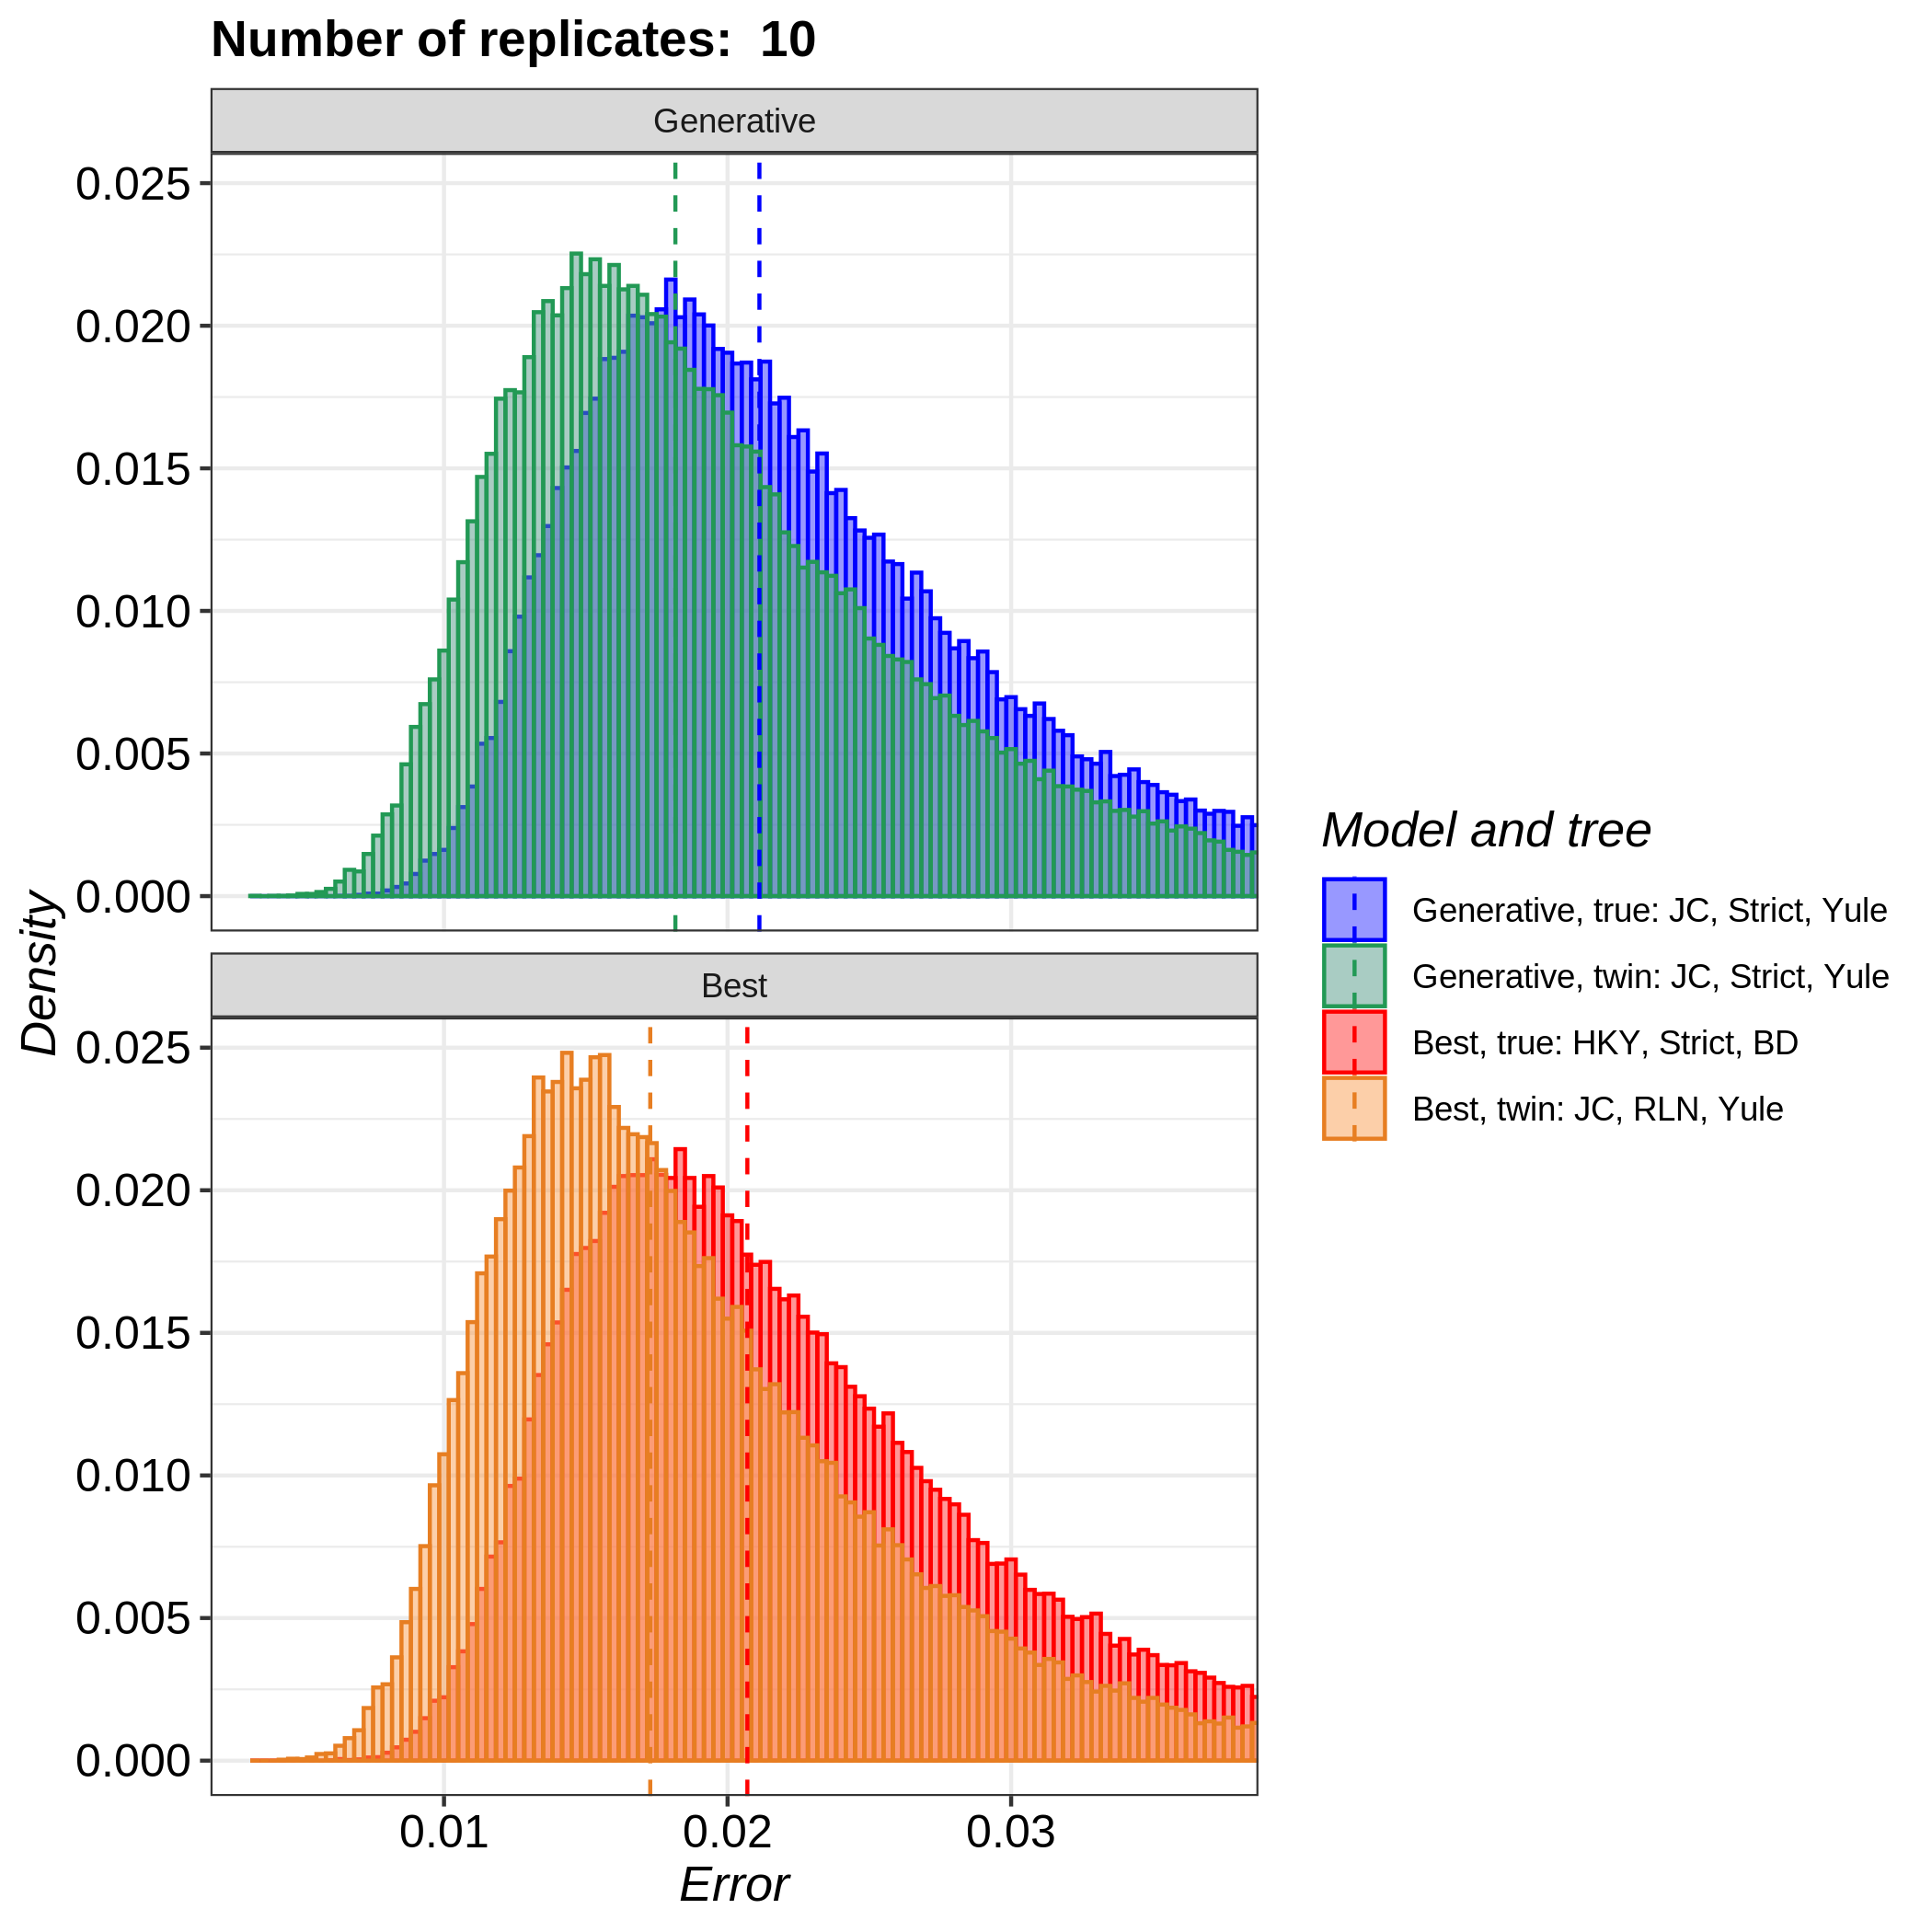
\includegraphics[width=\textwidth]{pirouette_example_33/errors.png}
    \caption{Aggregate error distributions for 20 replicates. Here each true tree has 24 taxa. This took 28 hours to compute.}
\end{figure}

\begin{figure}[H]
  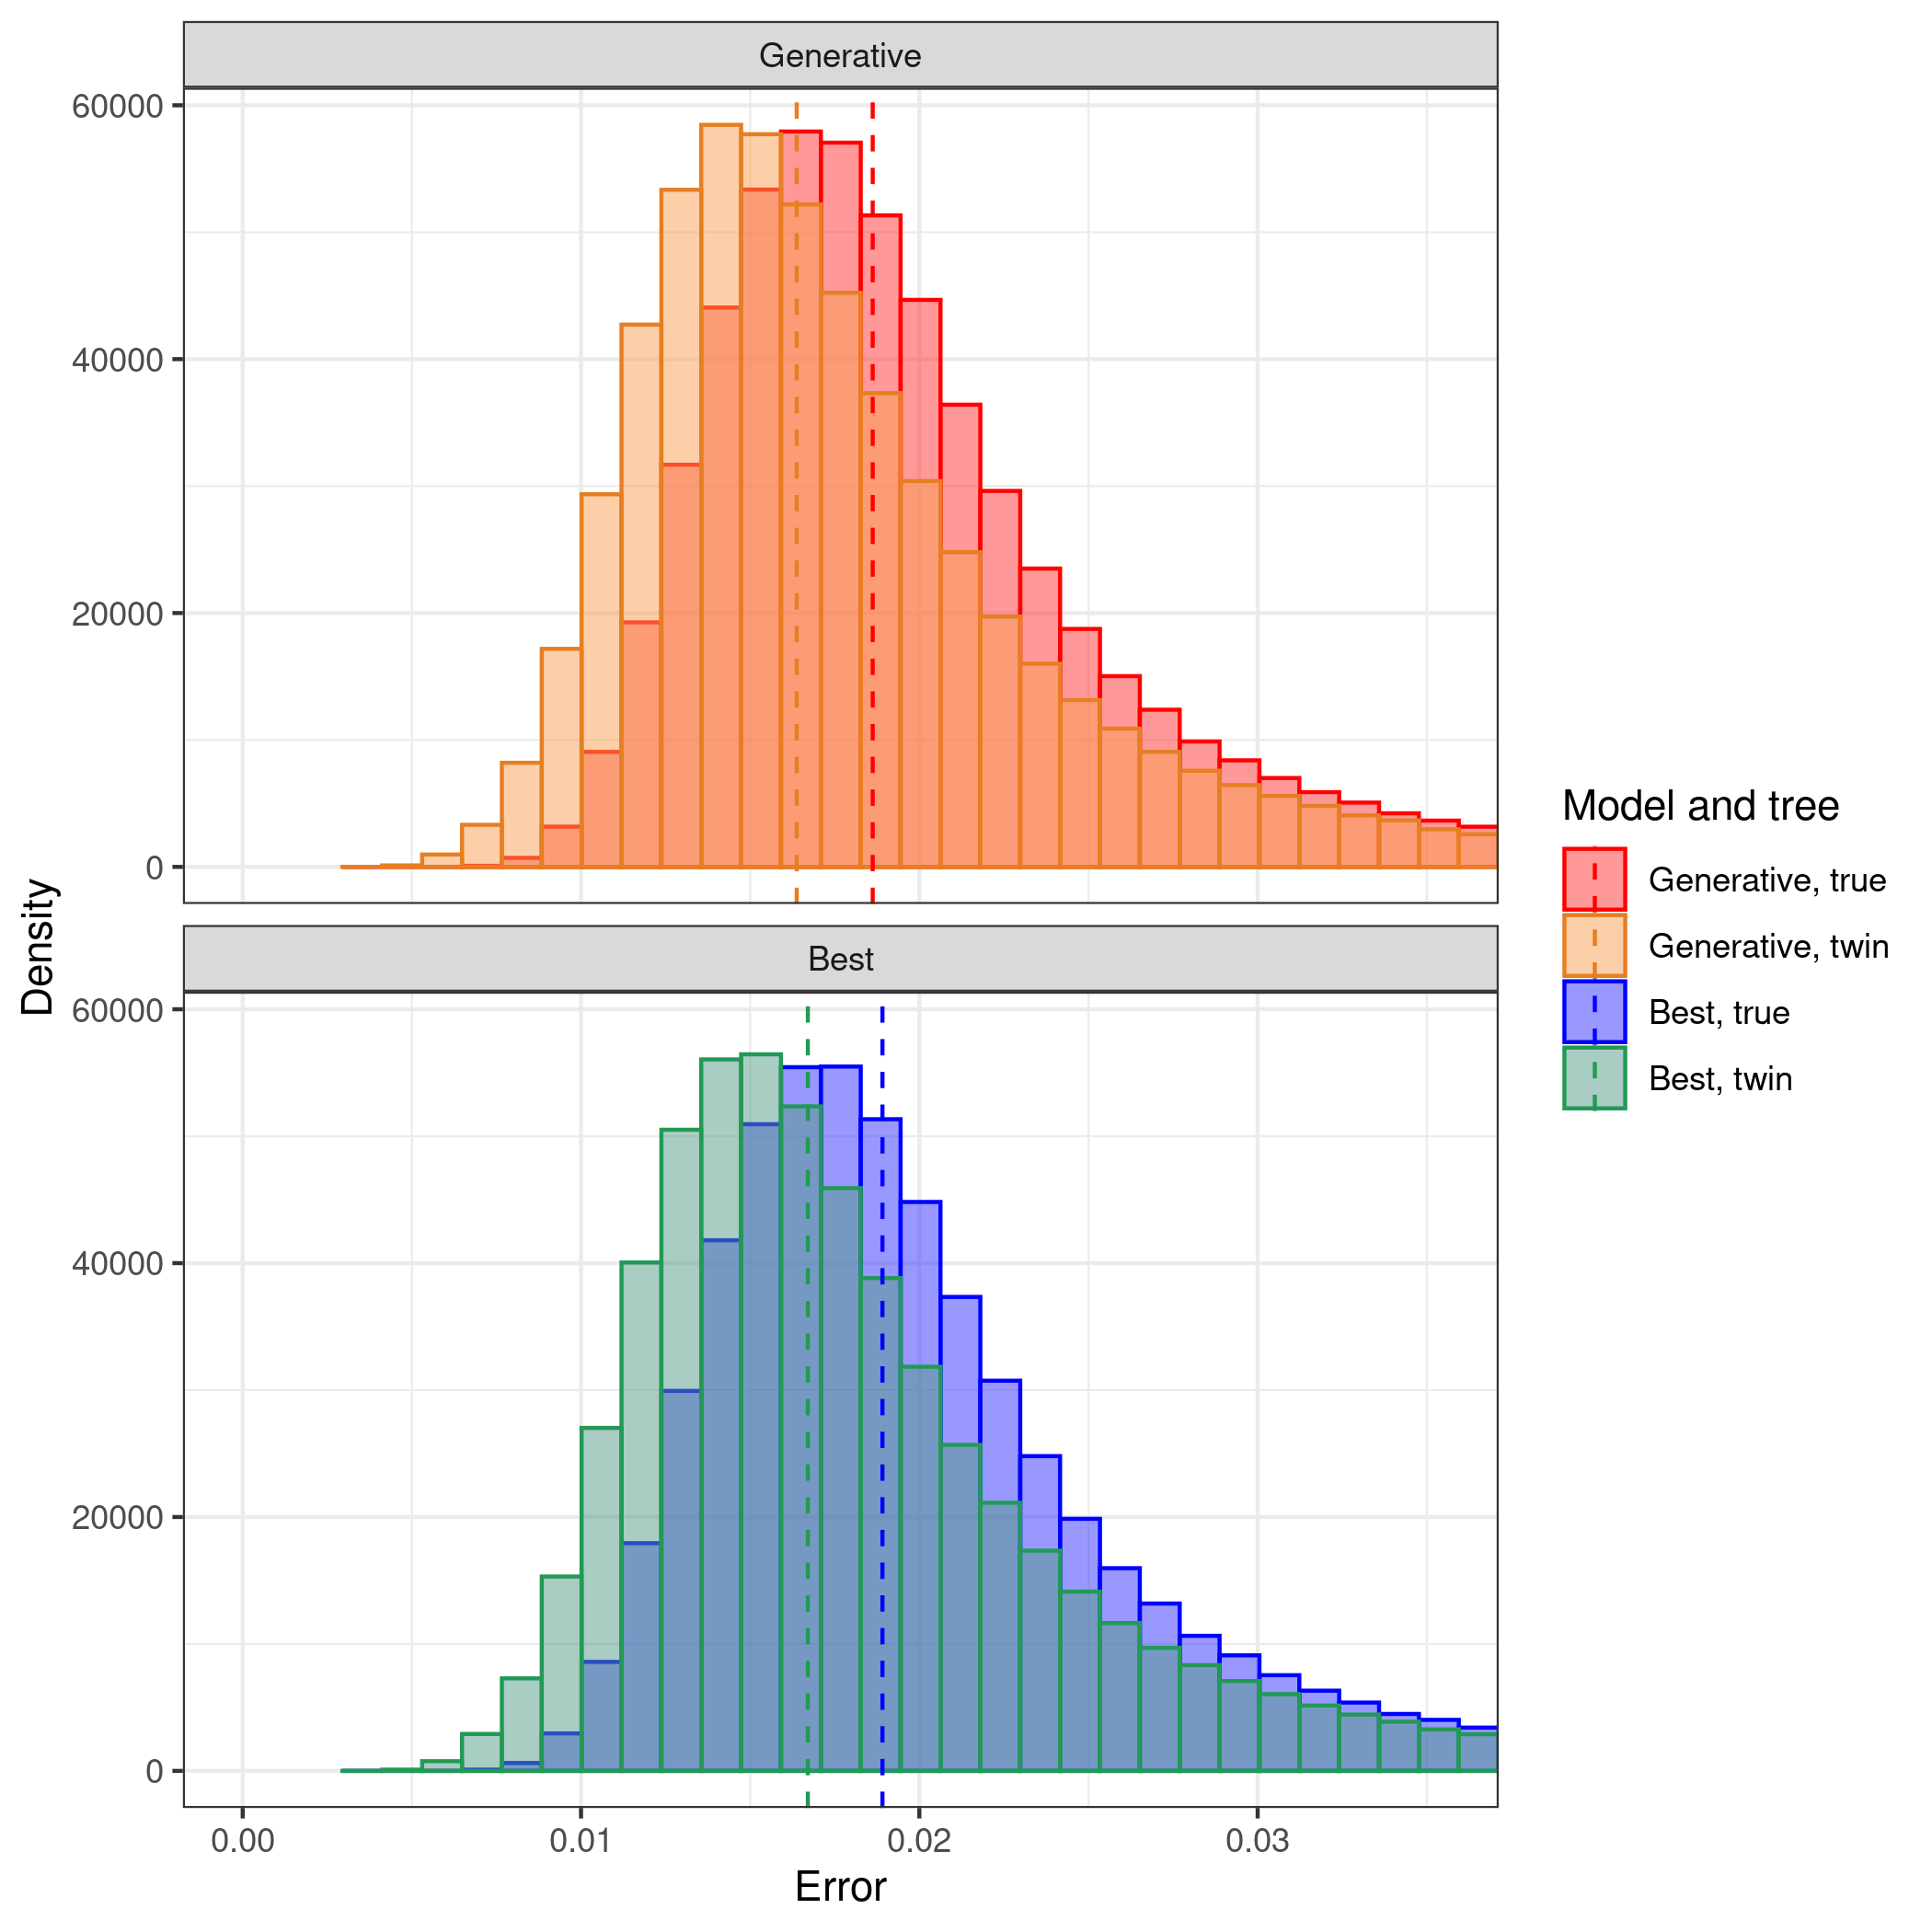
\includegraphics[width=\textwidth]{pirouette_example_41/errors.png}
  \caption{Aggregate error distributions for 5 replicates. Here each true tree has 32 taxa. This took 7 hours to compute.}
\end{figure}

\begin{figure}[H]
  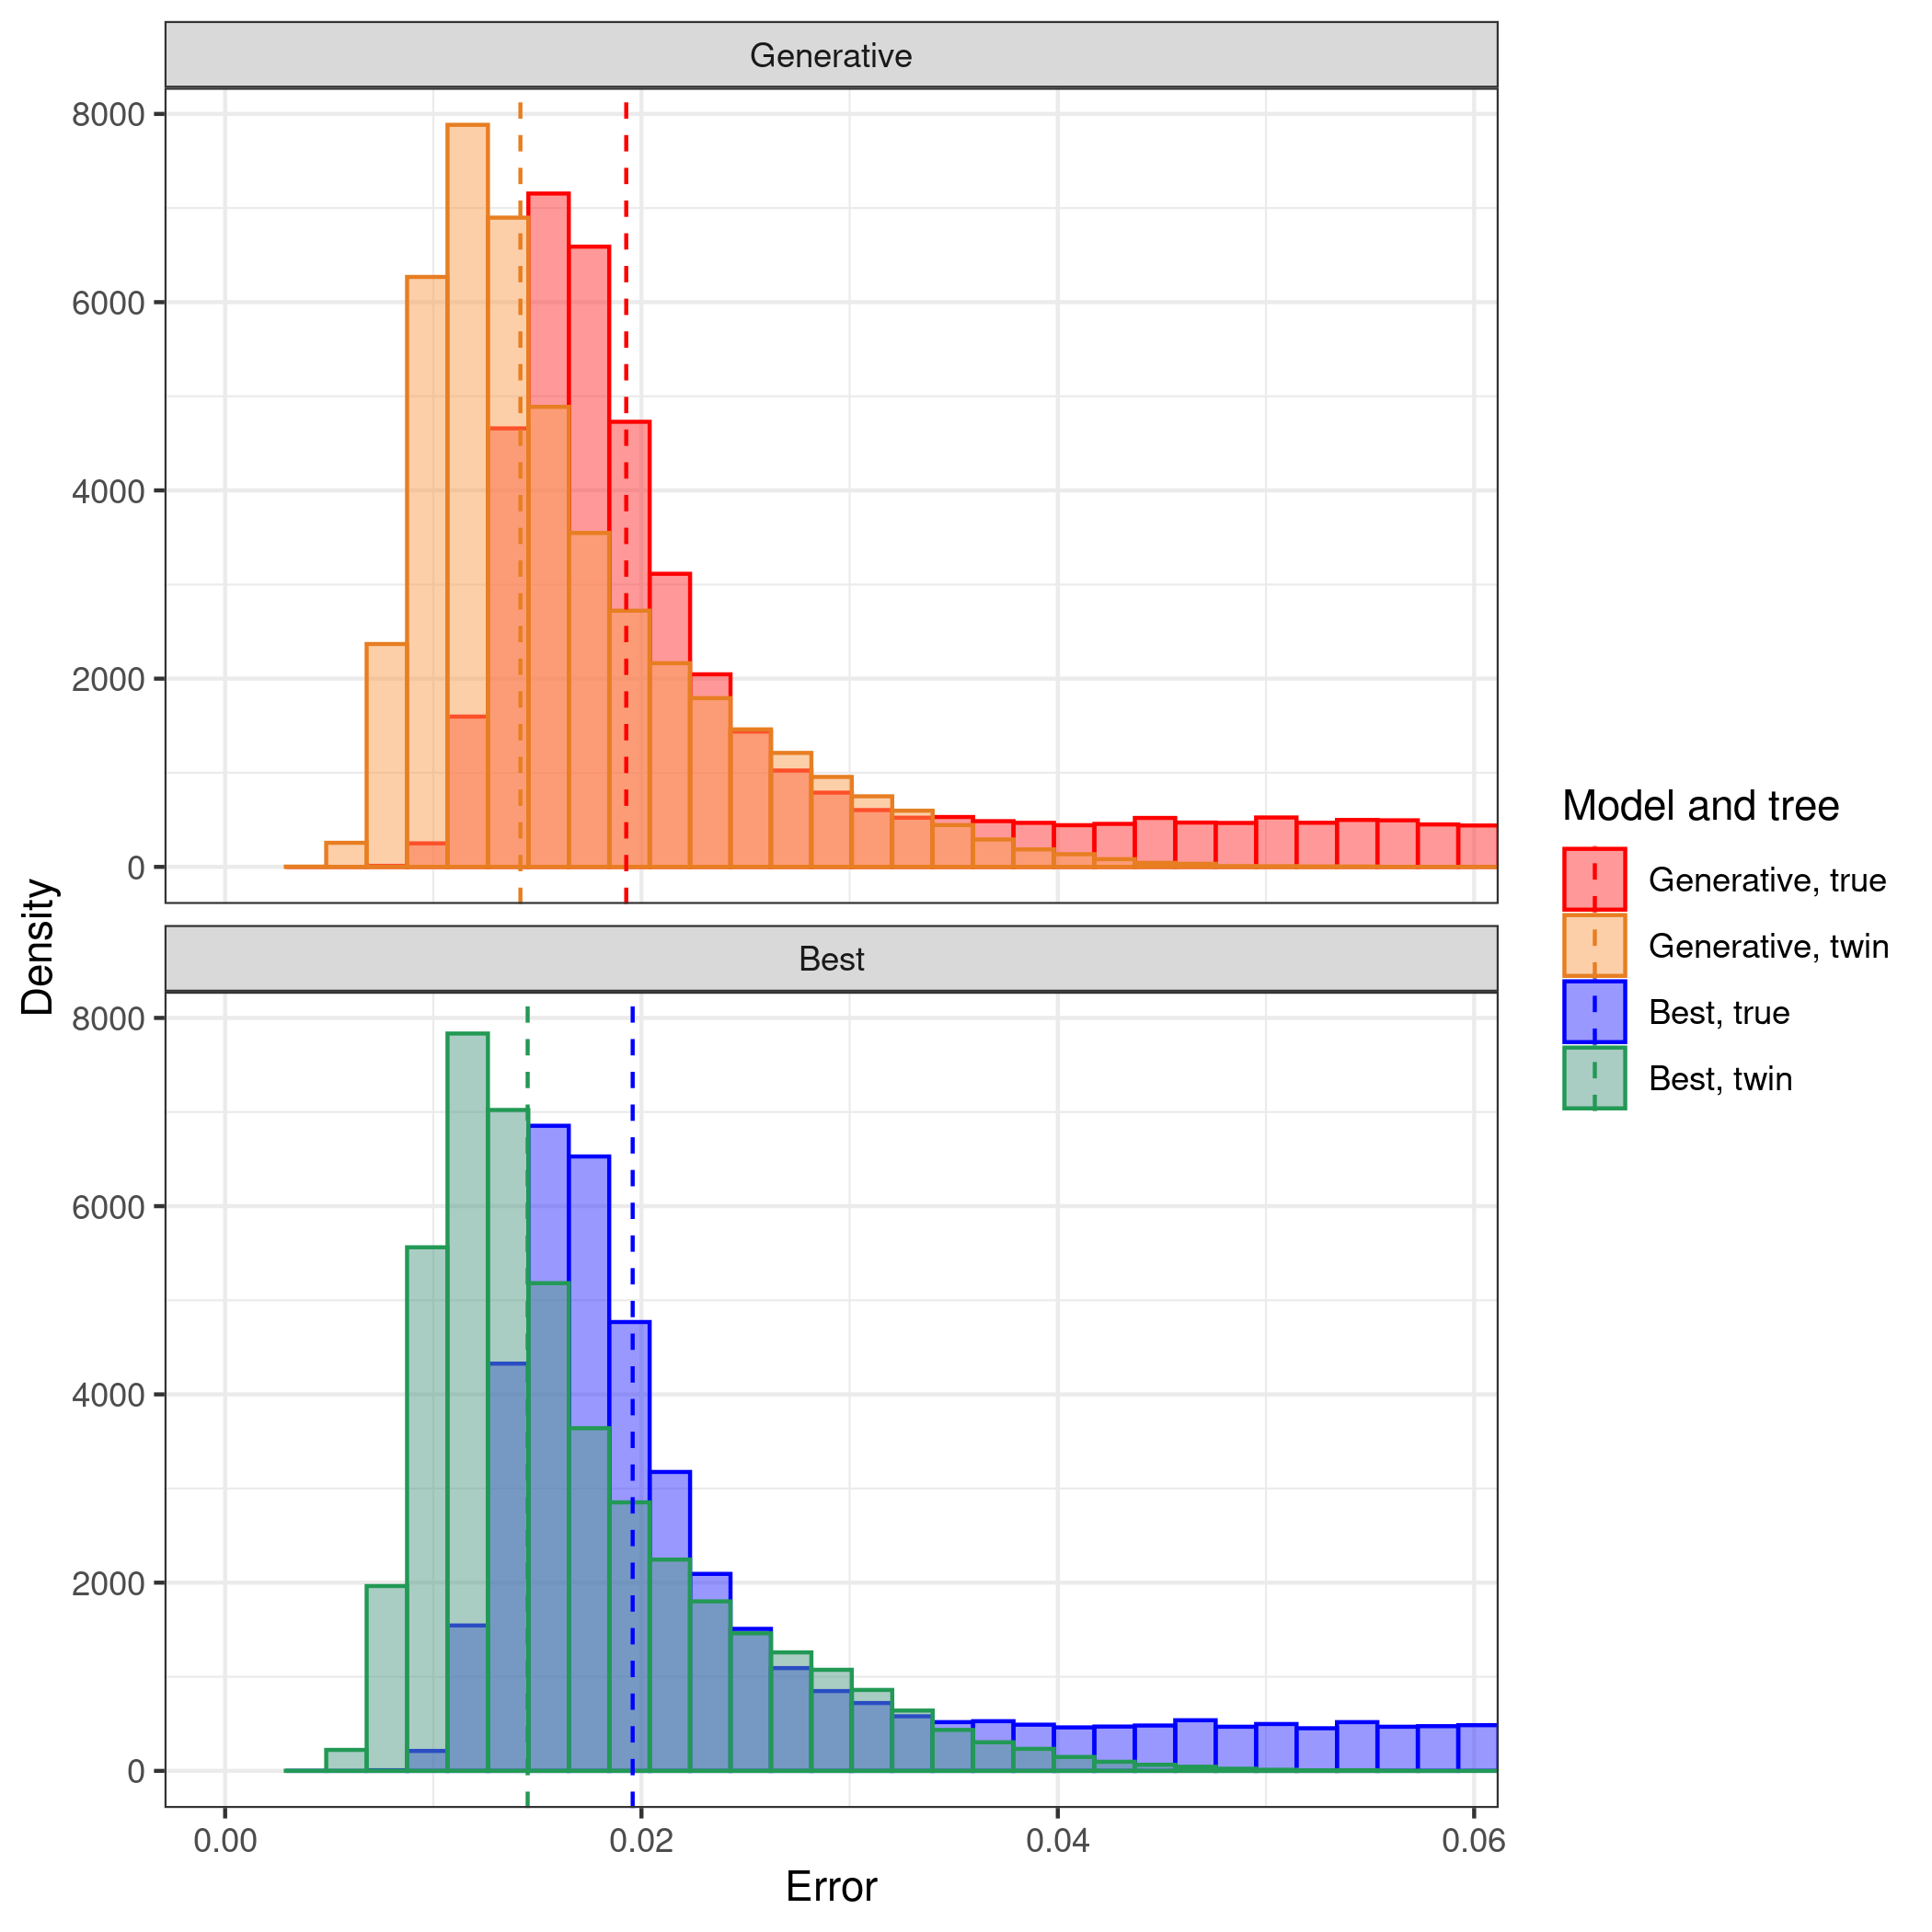
\includegraphics[width=\textwidth]{pirouette_example_42/errors.png}
  \caption{Aggregate error distributions for 2 replicates. Here each true tree has 40 taxa. This took 8 hours to compute.}
\end{figure}

%%%%%%%%%%%%%%%%%%%%%%%%%%%%%%%%%%%%%%%%%%%%%%%%%%%%%%%%%%%%%%%%%%%%%%%%%%%%%%%%
\subsection{The effect of DNA sequence length}
\label{subsec:n_nucleotides}
%%%%%%%%%%%%%%%%%%%%%%%%%%%%%%%%%%%%%%%%%%%%%%%%%%%%%%%%%%%%%%%%%%%%%%%%%%%%%%%%

The main example uses a DNA alignment length of 1000 nucleotides.
Here, we show the same results as the main example,
except for a varying DNA alignment sequence length.

The code to reproduce these figures can be found at  
\url{https://github.com/richelbilderbeek/pirouette_example_19} (500 nucleotides),
\url{https://github.com/richelbilderbeek/pirouette_example_28} (1000 nucleotides, main example),
and \url{https://github.com/richelbilderbeek/pirouette_example_34} (2000 nucleotides).

\begin{figure}[H]
  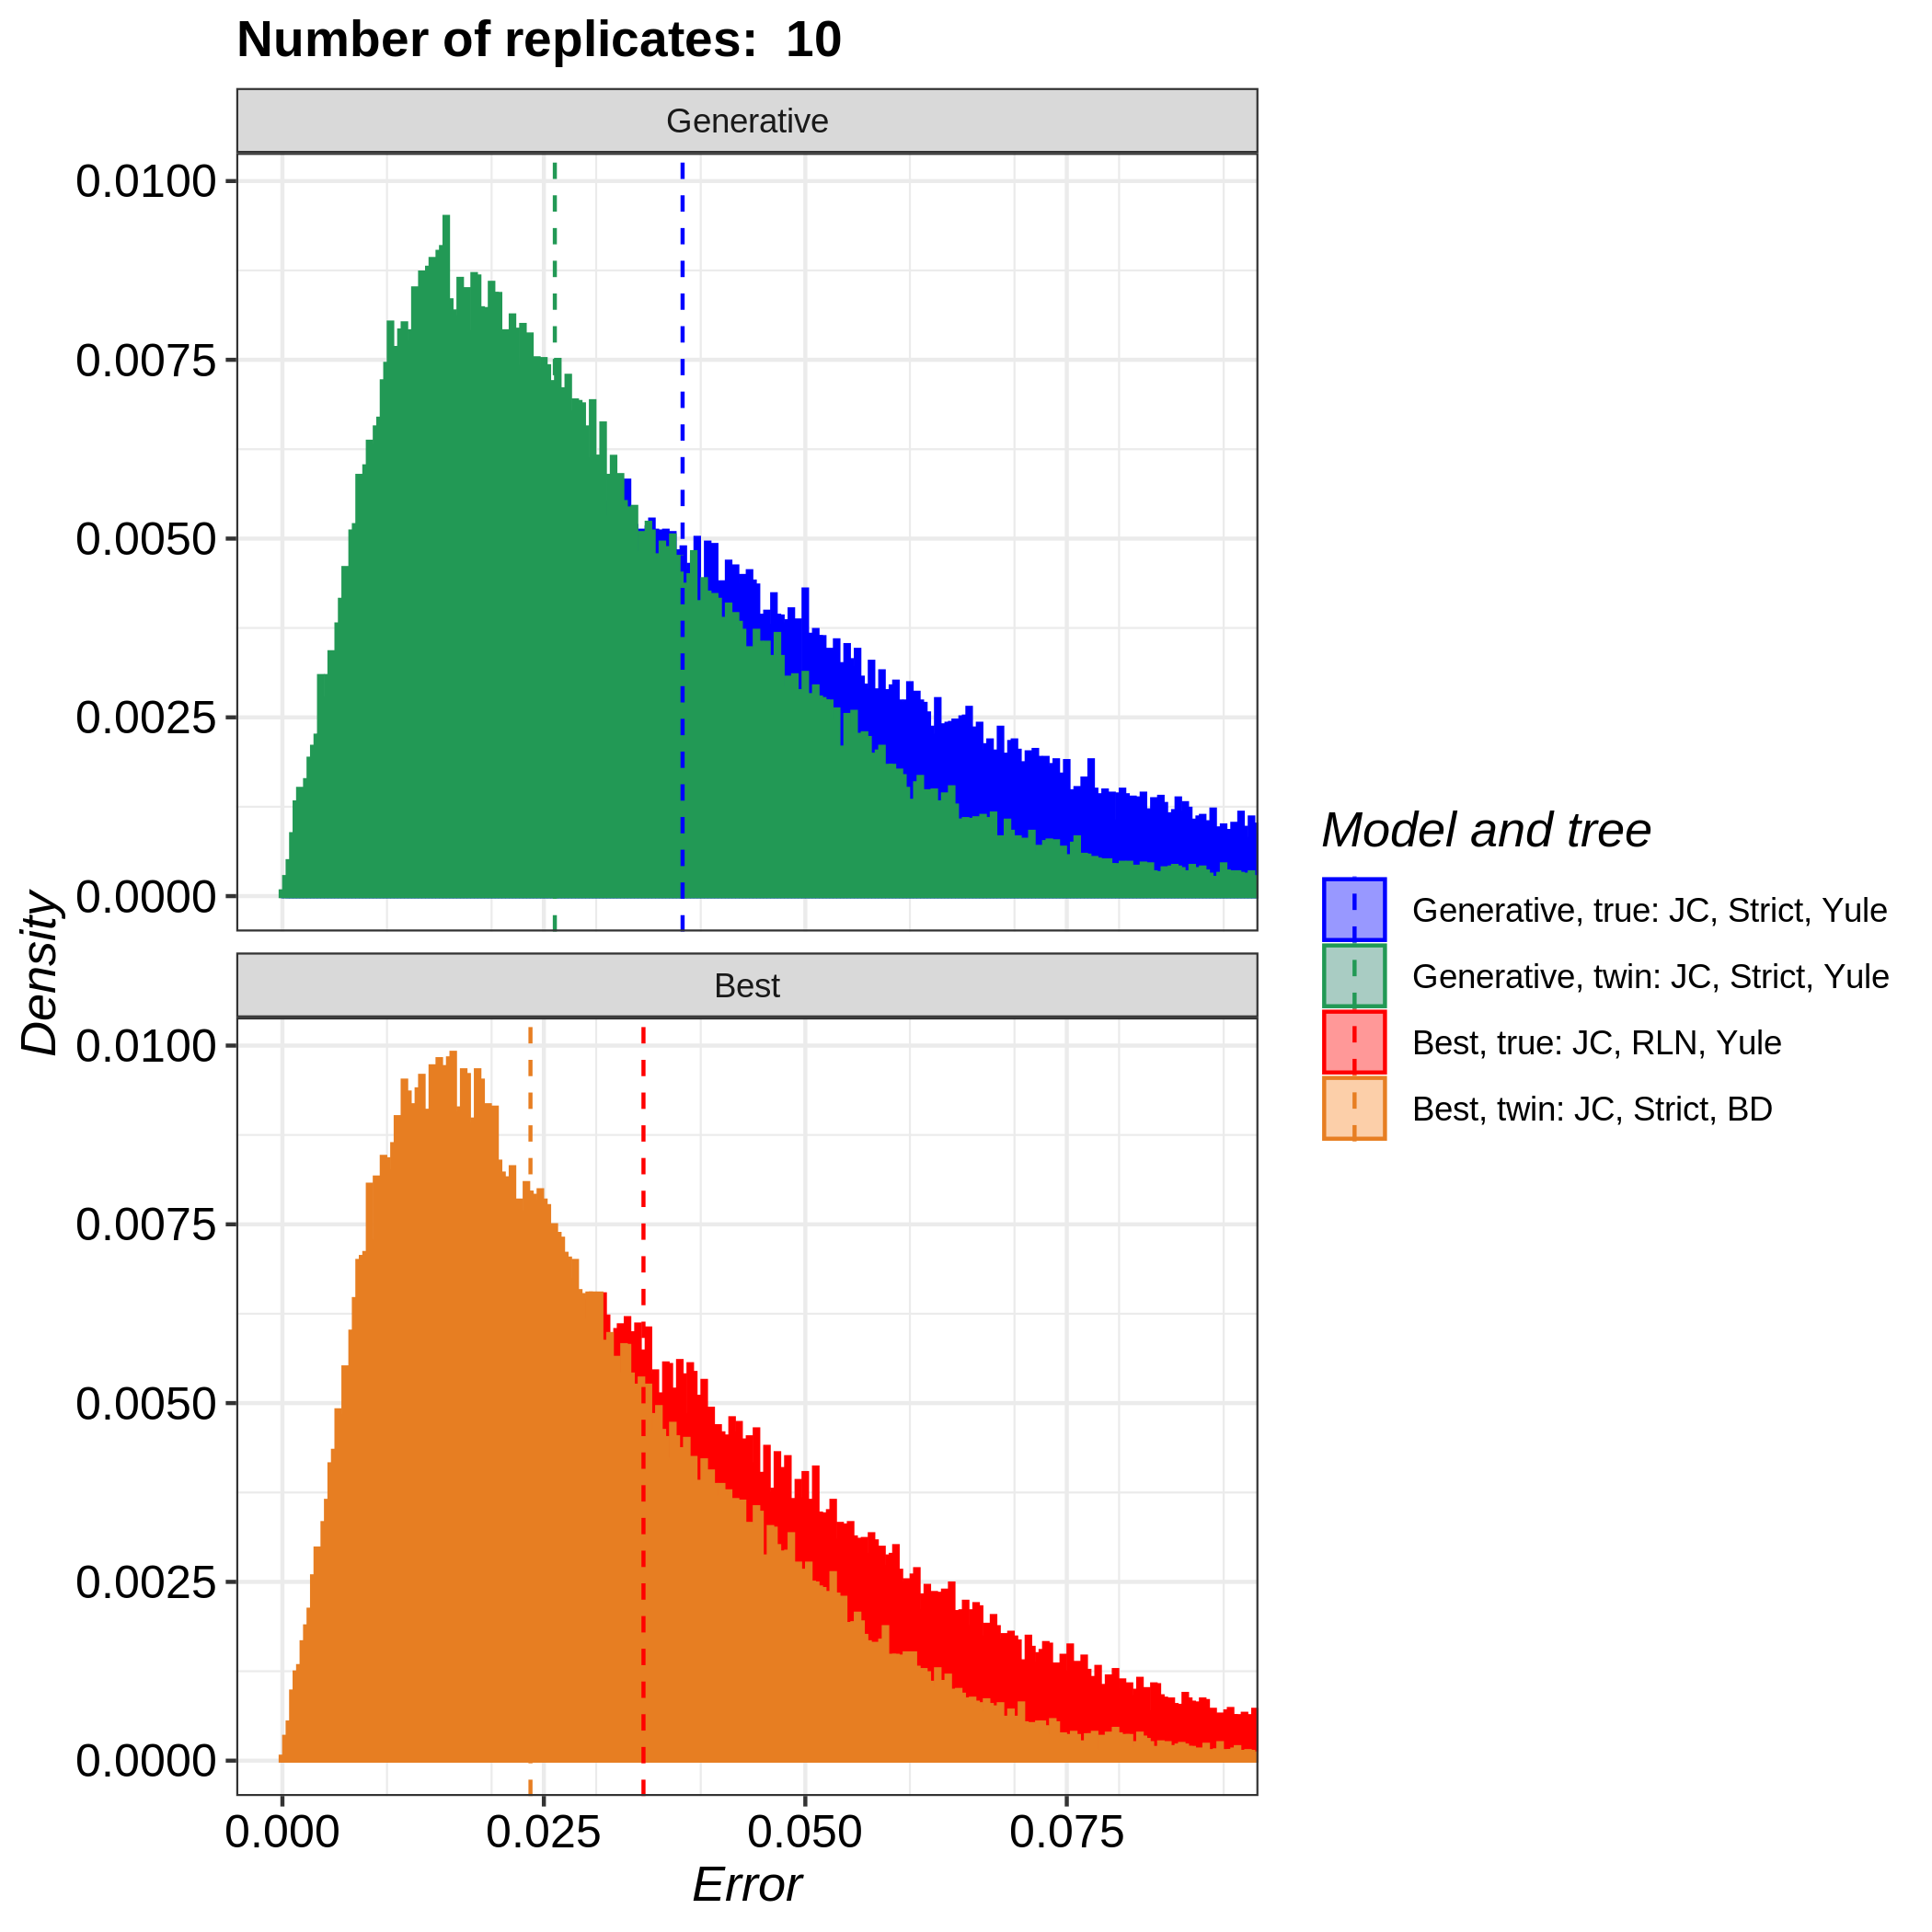
\includegraphics[width=\textwidth]{pirouette_example_19/errors.png}
  \caption{Aggregate error distributions for 20 replicates. Here each each alignment has a sequence length of 500 nucleotides. This took 12 hours to compute.}
\end{figure}

\begin{figure}[H]
  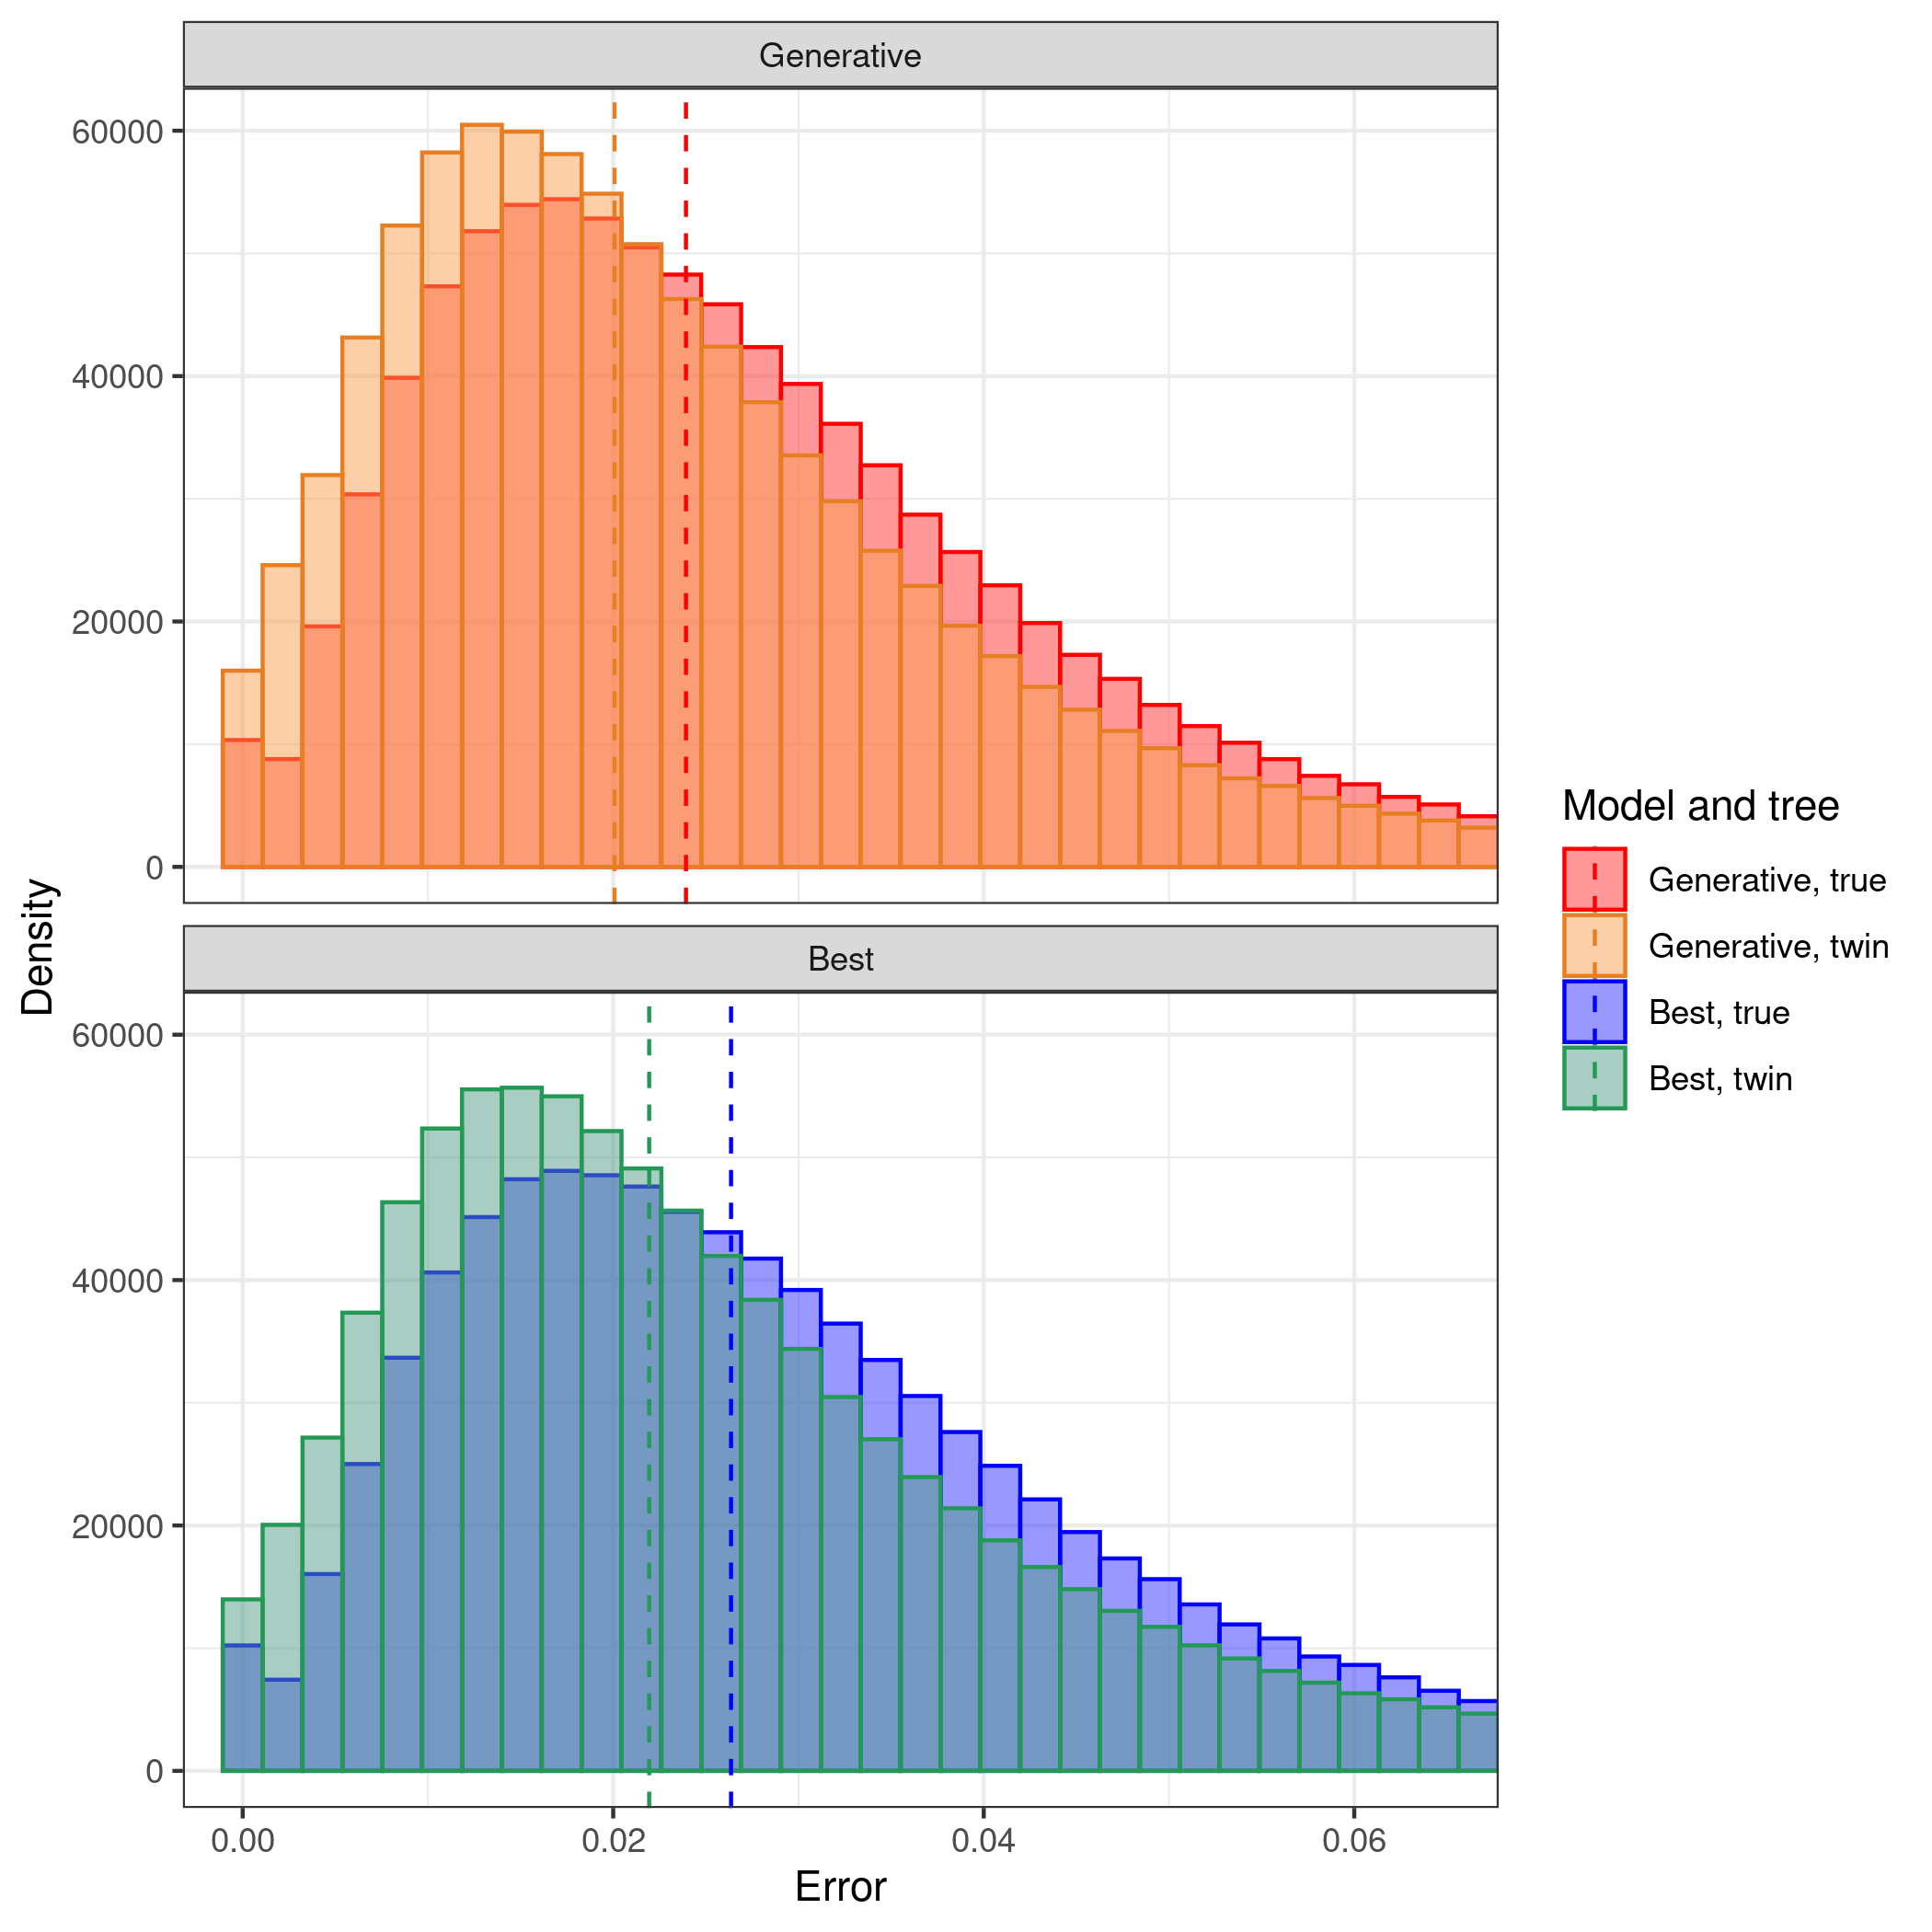
\includegraphics[width=\textwidth]{pirouette_example_28/errors.png}
  \caption{Aggregate error distributions for 20 replicates. Here each each alignment has a sequence length of 1000 nucleotides (as used in the main example). This took 16 hours to compute.}
\end{figure}

\begin{figure}[H]
  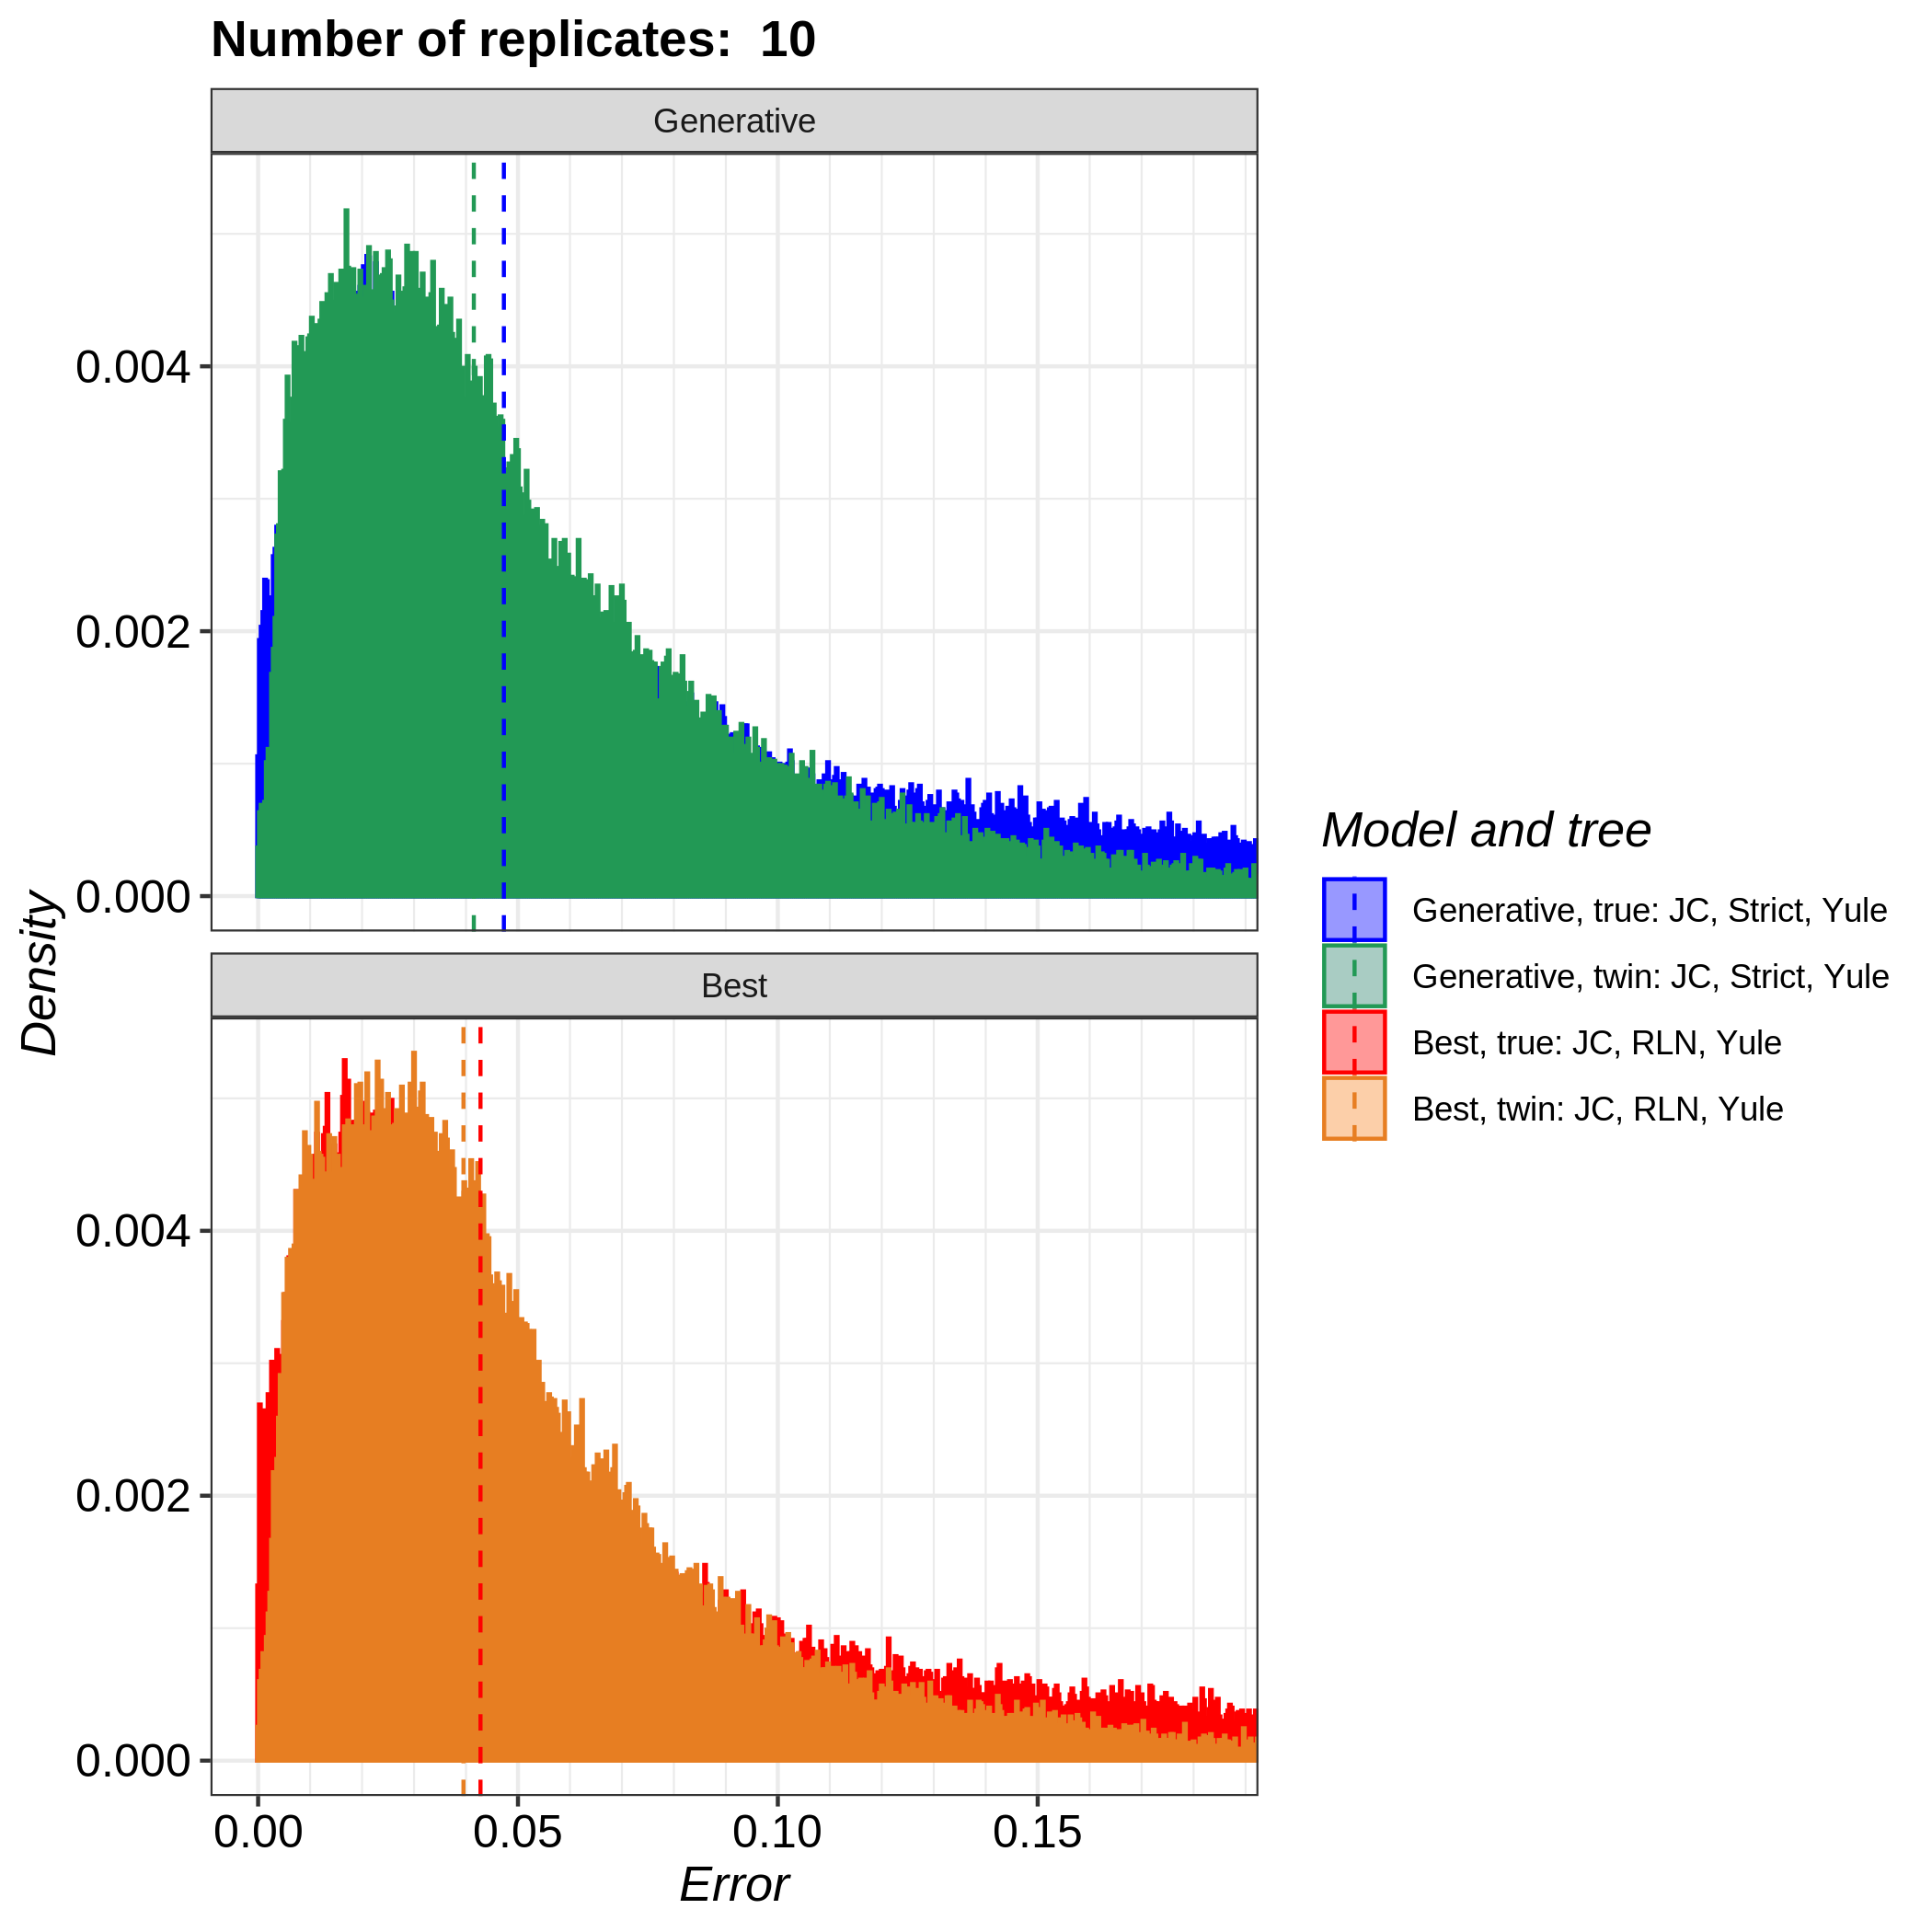
\includegraphics[width=\textwidth]{pirouette_example_34/errors.png}
  \caption{Aggregate error distributions for 10 replicates. Here each each alignment has a sequence length of 2000 nucleotides. This took 11 hours to compute.}
\end{figure}

%%%%%%%%%%%%%%%%%%%%%%%%%%%%%%%%%%%%%%%%%%%%%%%%%%%%%%%%%%%%%%%%%%%%%%%%%%%%%%%%
\subsection{The effect of assuming a Yule tree prior on a Yule tree}
\label{subsec:simplest_correct_parameterization}
%%%%%%%%%%%%%%%%%%%%%%%%%%%%%%%%%%%%%%%%%%%%%%%%%%%%%%%%%%%%%%%%%%%%%%%%%%%%%%%%

The main example uses a tree generated by a non-standard tree model.
Here, we show the same results, with the only difference that
the tree used is generated by simplest tree model (the Yule model),
which we also assume as the (correct) tree prior.
This example thus shows a parameterization at the correct level for the
simplest case possible.

The code to reproduce this figure can be found at  
\url{https://github.com/richelbilderbeek/pirouette_example_22}.

\begin{figure}[H]
  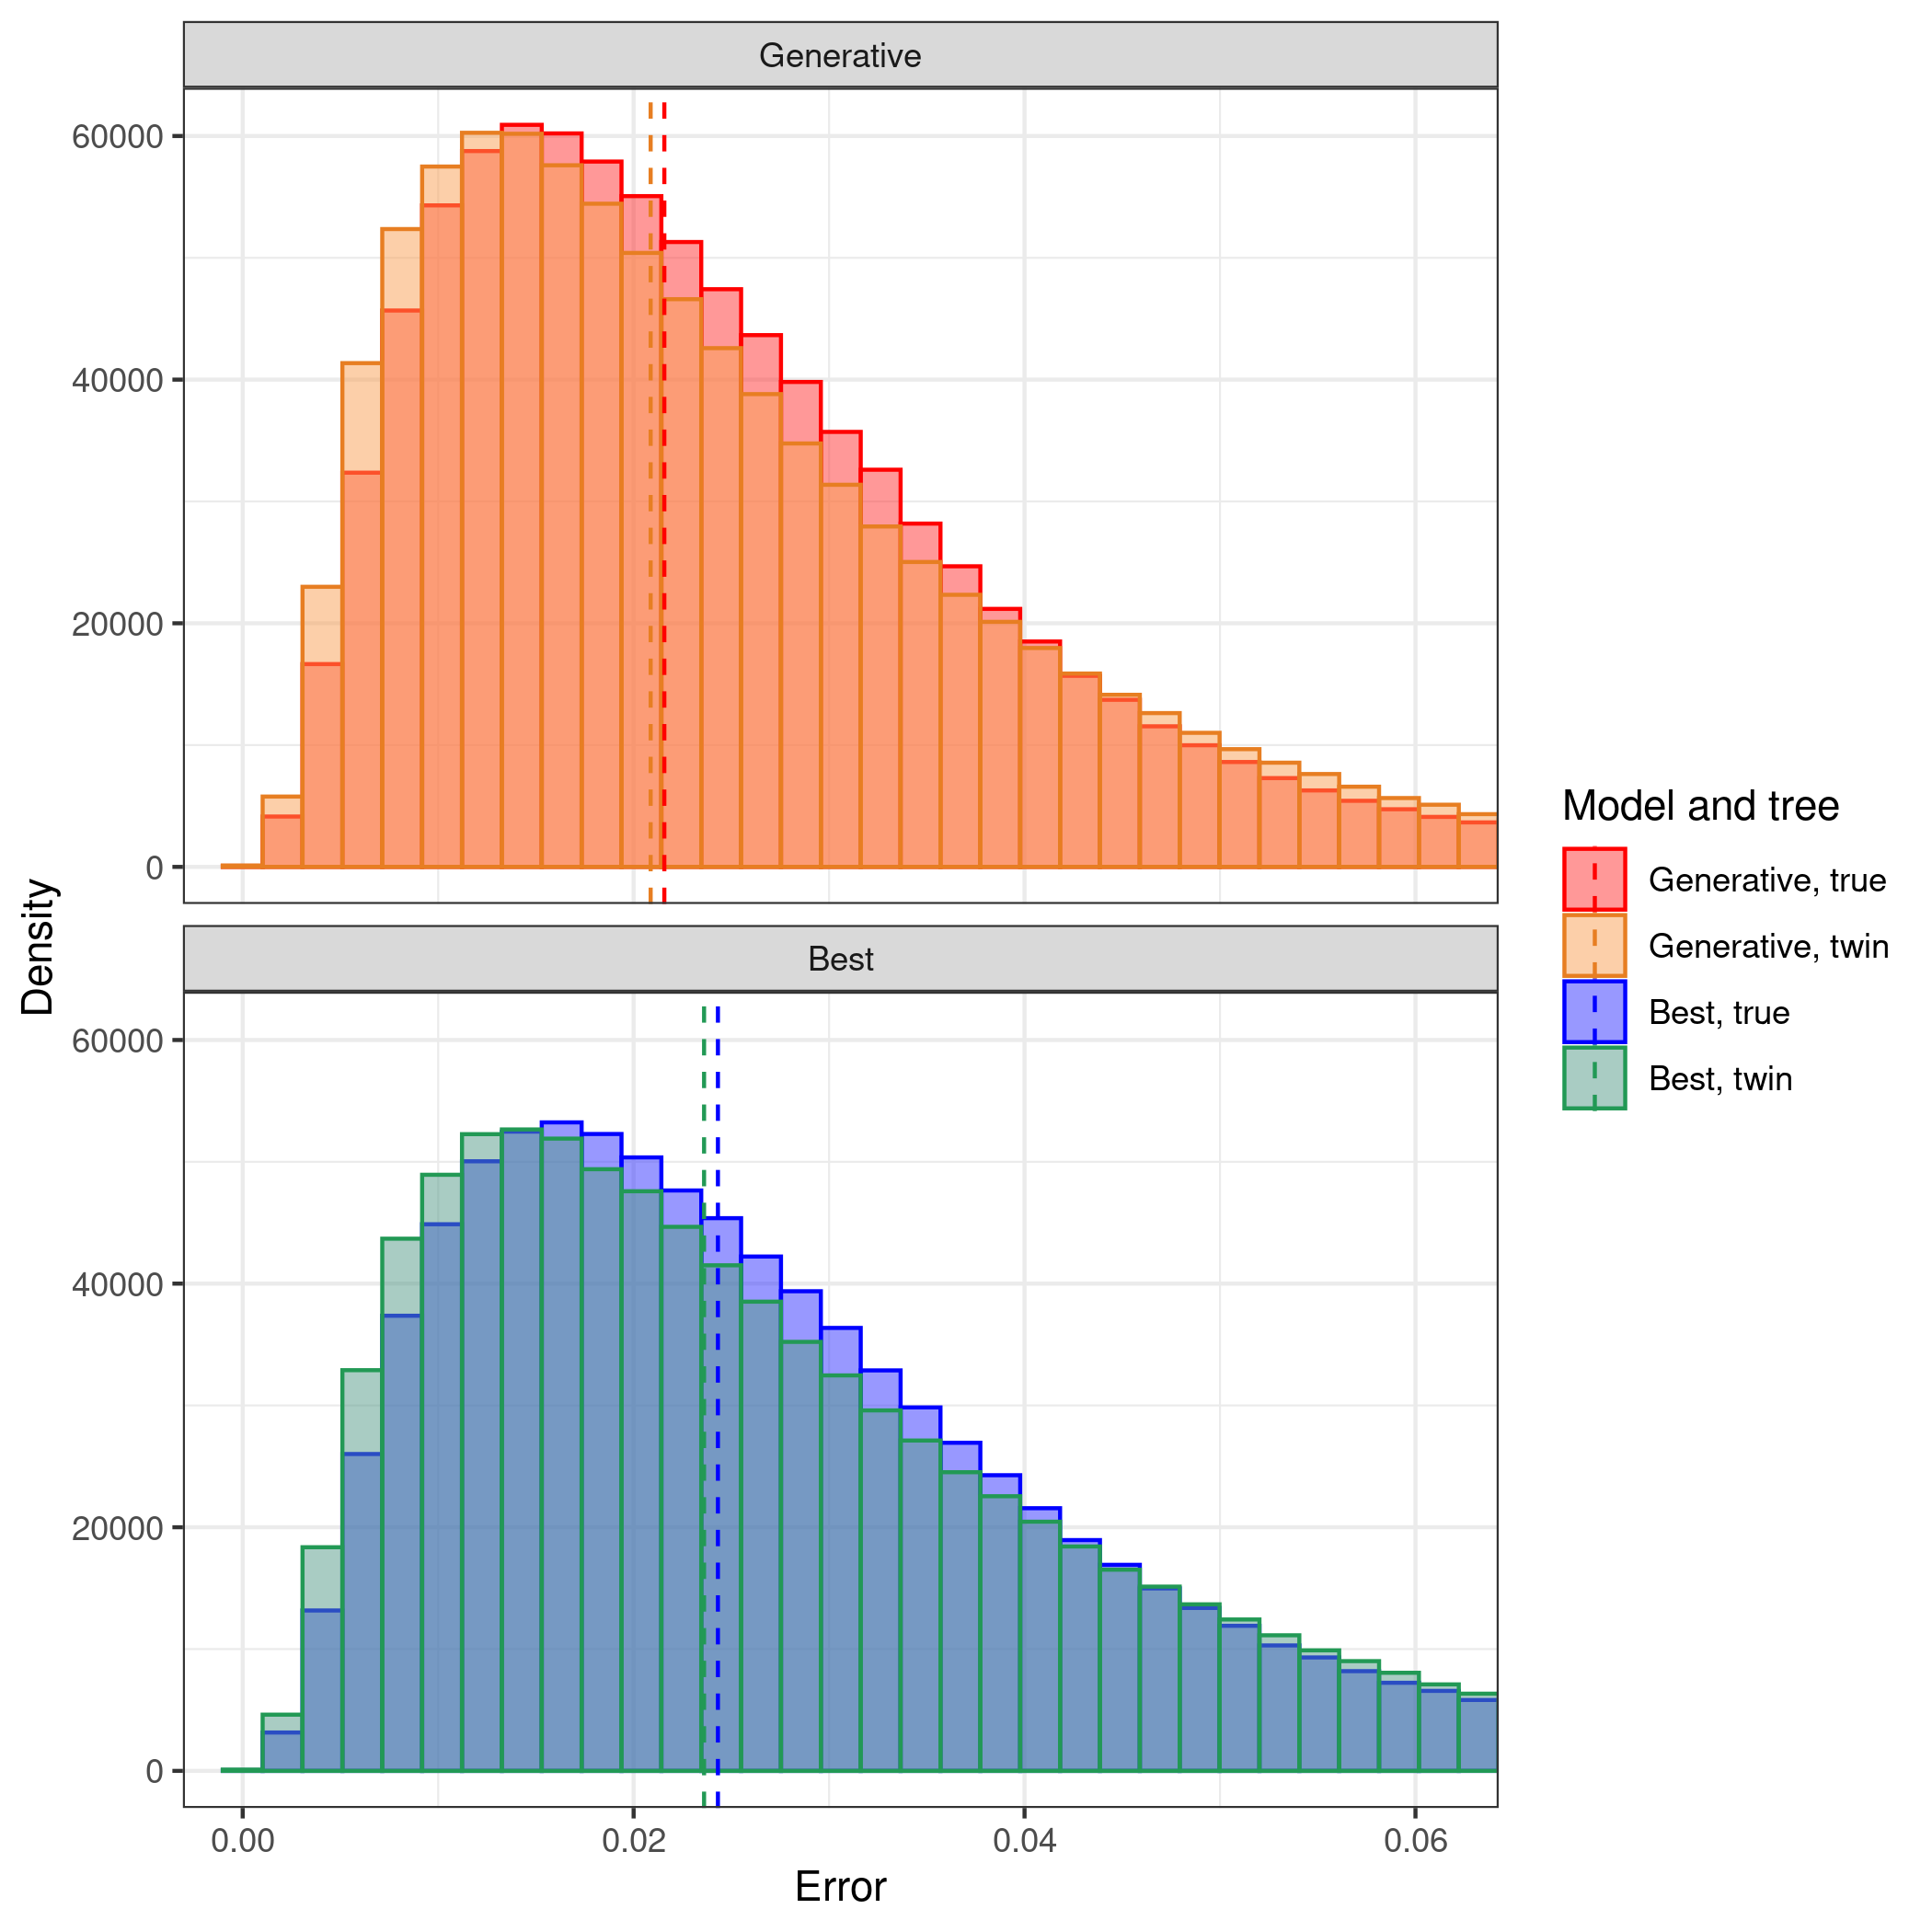
\includegraphics[width=\textwidth]{pirouette_example_22/errors.png}
  \caption{Aggregate error distributions for 10 replicates. Here each true tree is generated by a Yule process. For the inference we used a Yule tree prior. This took 9 hours to compute.}
\end{figure}

%%%%%%%%%%%%%%%%%%%%%%%%%%%%%%%%%%%%%%%%%%%%%%%%%%%%%%%%%%%%%%%%%%%%%%%%%%%%%%%%
\subsection{The effect of assuming a Yule tree prior on a BD tree}
\label{subsec:under_parameterization}
%%%%%%%%%%%%%%%%%%%%%%%%%%%%%%%%%%%%%%%%%%%%%%%%%%%%%%%%%%%%%%%%%%%%%%%%%%%%%%%%

The main example uses a tree generated by a non-standard tree model.

Here, we show the same results, with the difference that
the tree used is generated by a birth-death (BD) tree model,
where we assume it is generated by a Yule (or pure-birth) model.
This example thus shows the effect of underparameterization.

The code to reproduce this figure can be found at  
\url{https://github.com/richelbilderbeek/pirouette_example_26}.

\begin{figure}[H]
  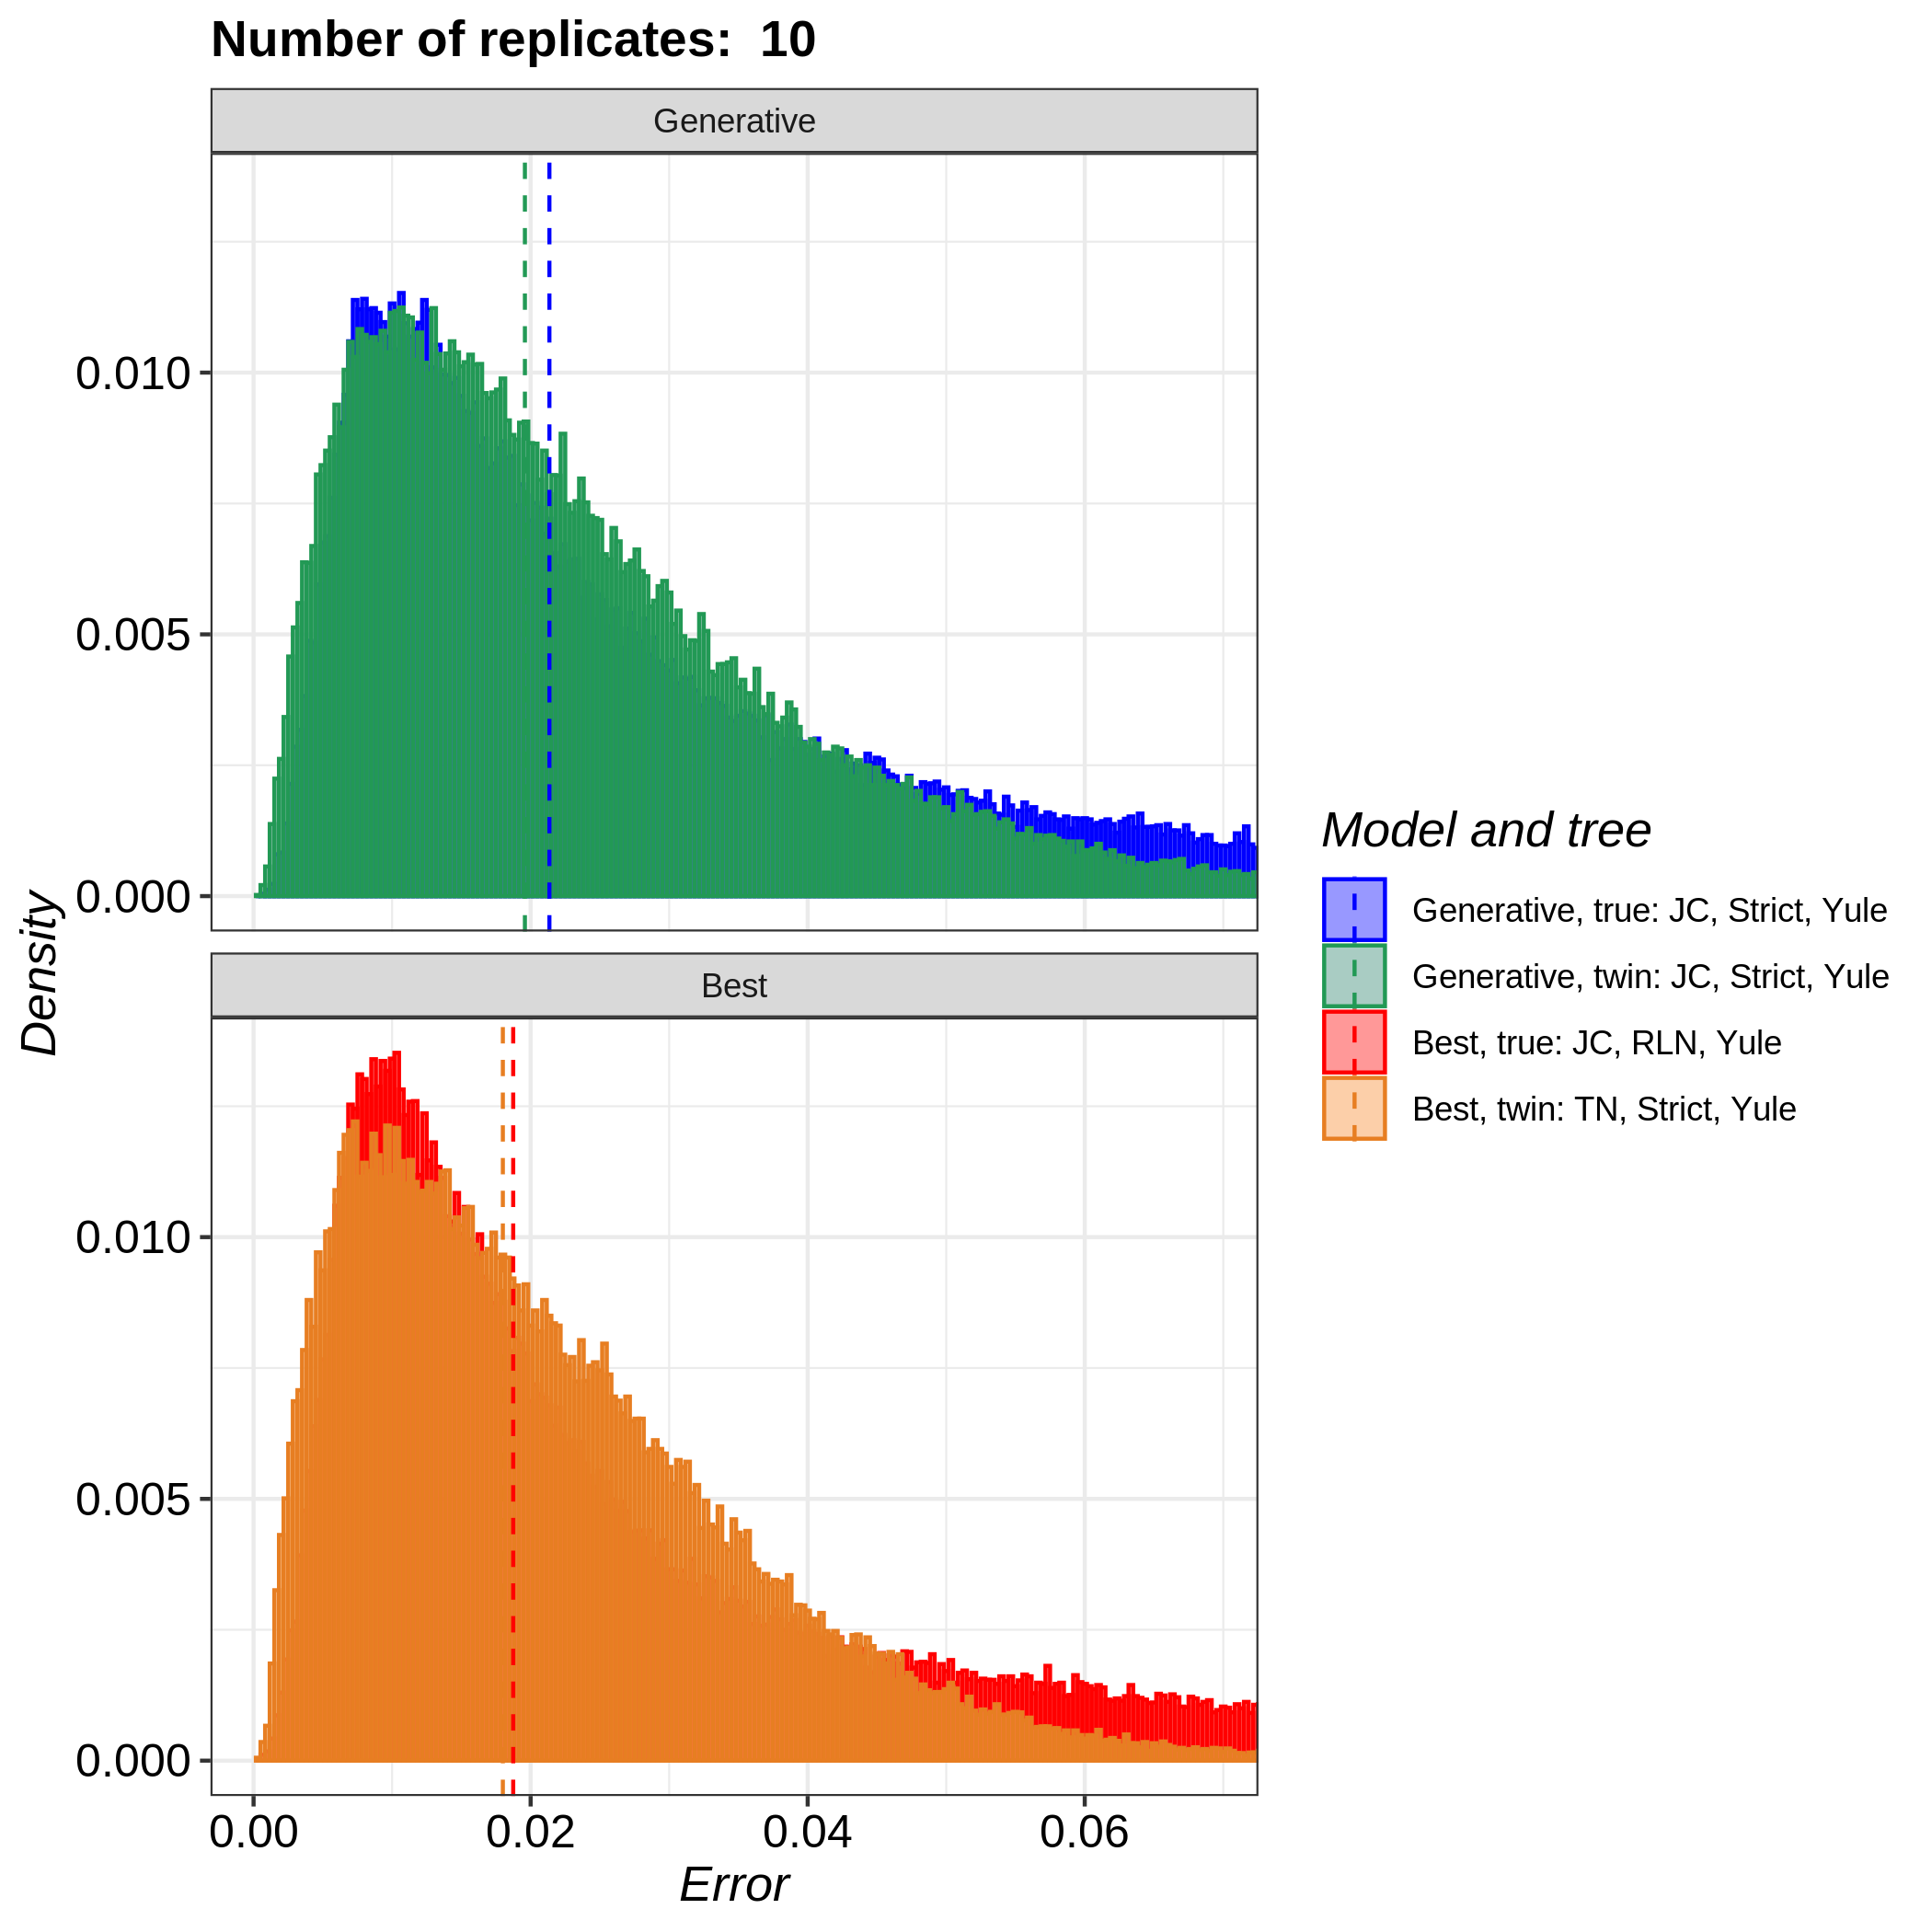
\includegraphics[width=\textwidth]{pirouette_example_26/errors.png}
  \caption{Aggregate error distributions for 20 replicates. Here each true tree is generated by a BD process. For the inference we used instead a Yule tree prior. This took 9 hours to compute.}
\end{figure}

%%%%%%%%%%%%%%%%%%%%%%%%%%%%%%%%%%%%%%%%%%%%%%%%%%%%%%%%%%%%%%%%%%%%%%%%%%%%%%%%
\subsection{The effect of diversity-dependent trees differing in how likely they are under the DD process}
\label{subsec:better_label_needed}
%%%%%%%%%%%%%%%%%%%%%%%%%%%%%%%%%%%%%%%%%%%%%%%%%%%%%%%%%%%%%%%%%%%%%%%%%%%%%%%%

Here we show the results of a \verb;pirouette; run on a dataset 
of multiple DD trees that we selected for having a low, median
and high likelihood. In this way, we effectively selected for trees
that are rare, uncommon and common respectively.

The code to reproduce these figure can be found at  
\url{https://github.com/richelbilderbeek/pirouette_example_23}
and took 120 hours in total.

\begin{figure}[H]
  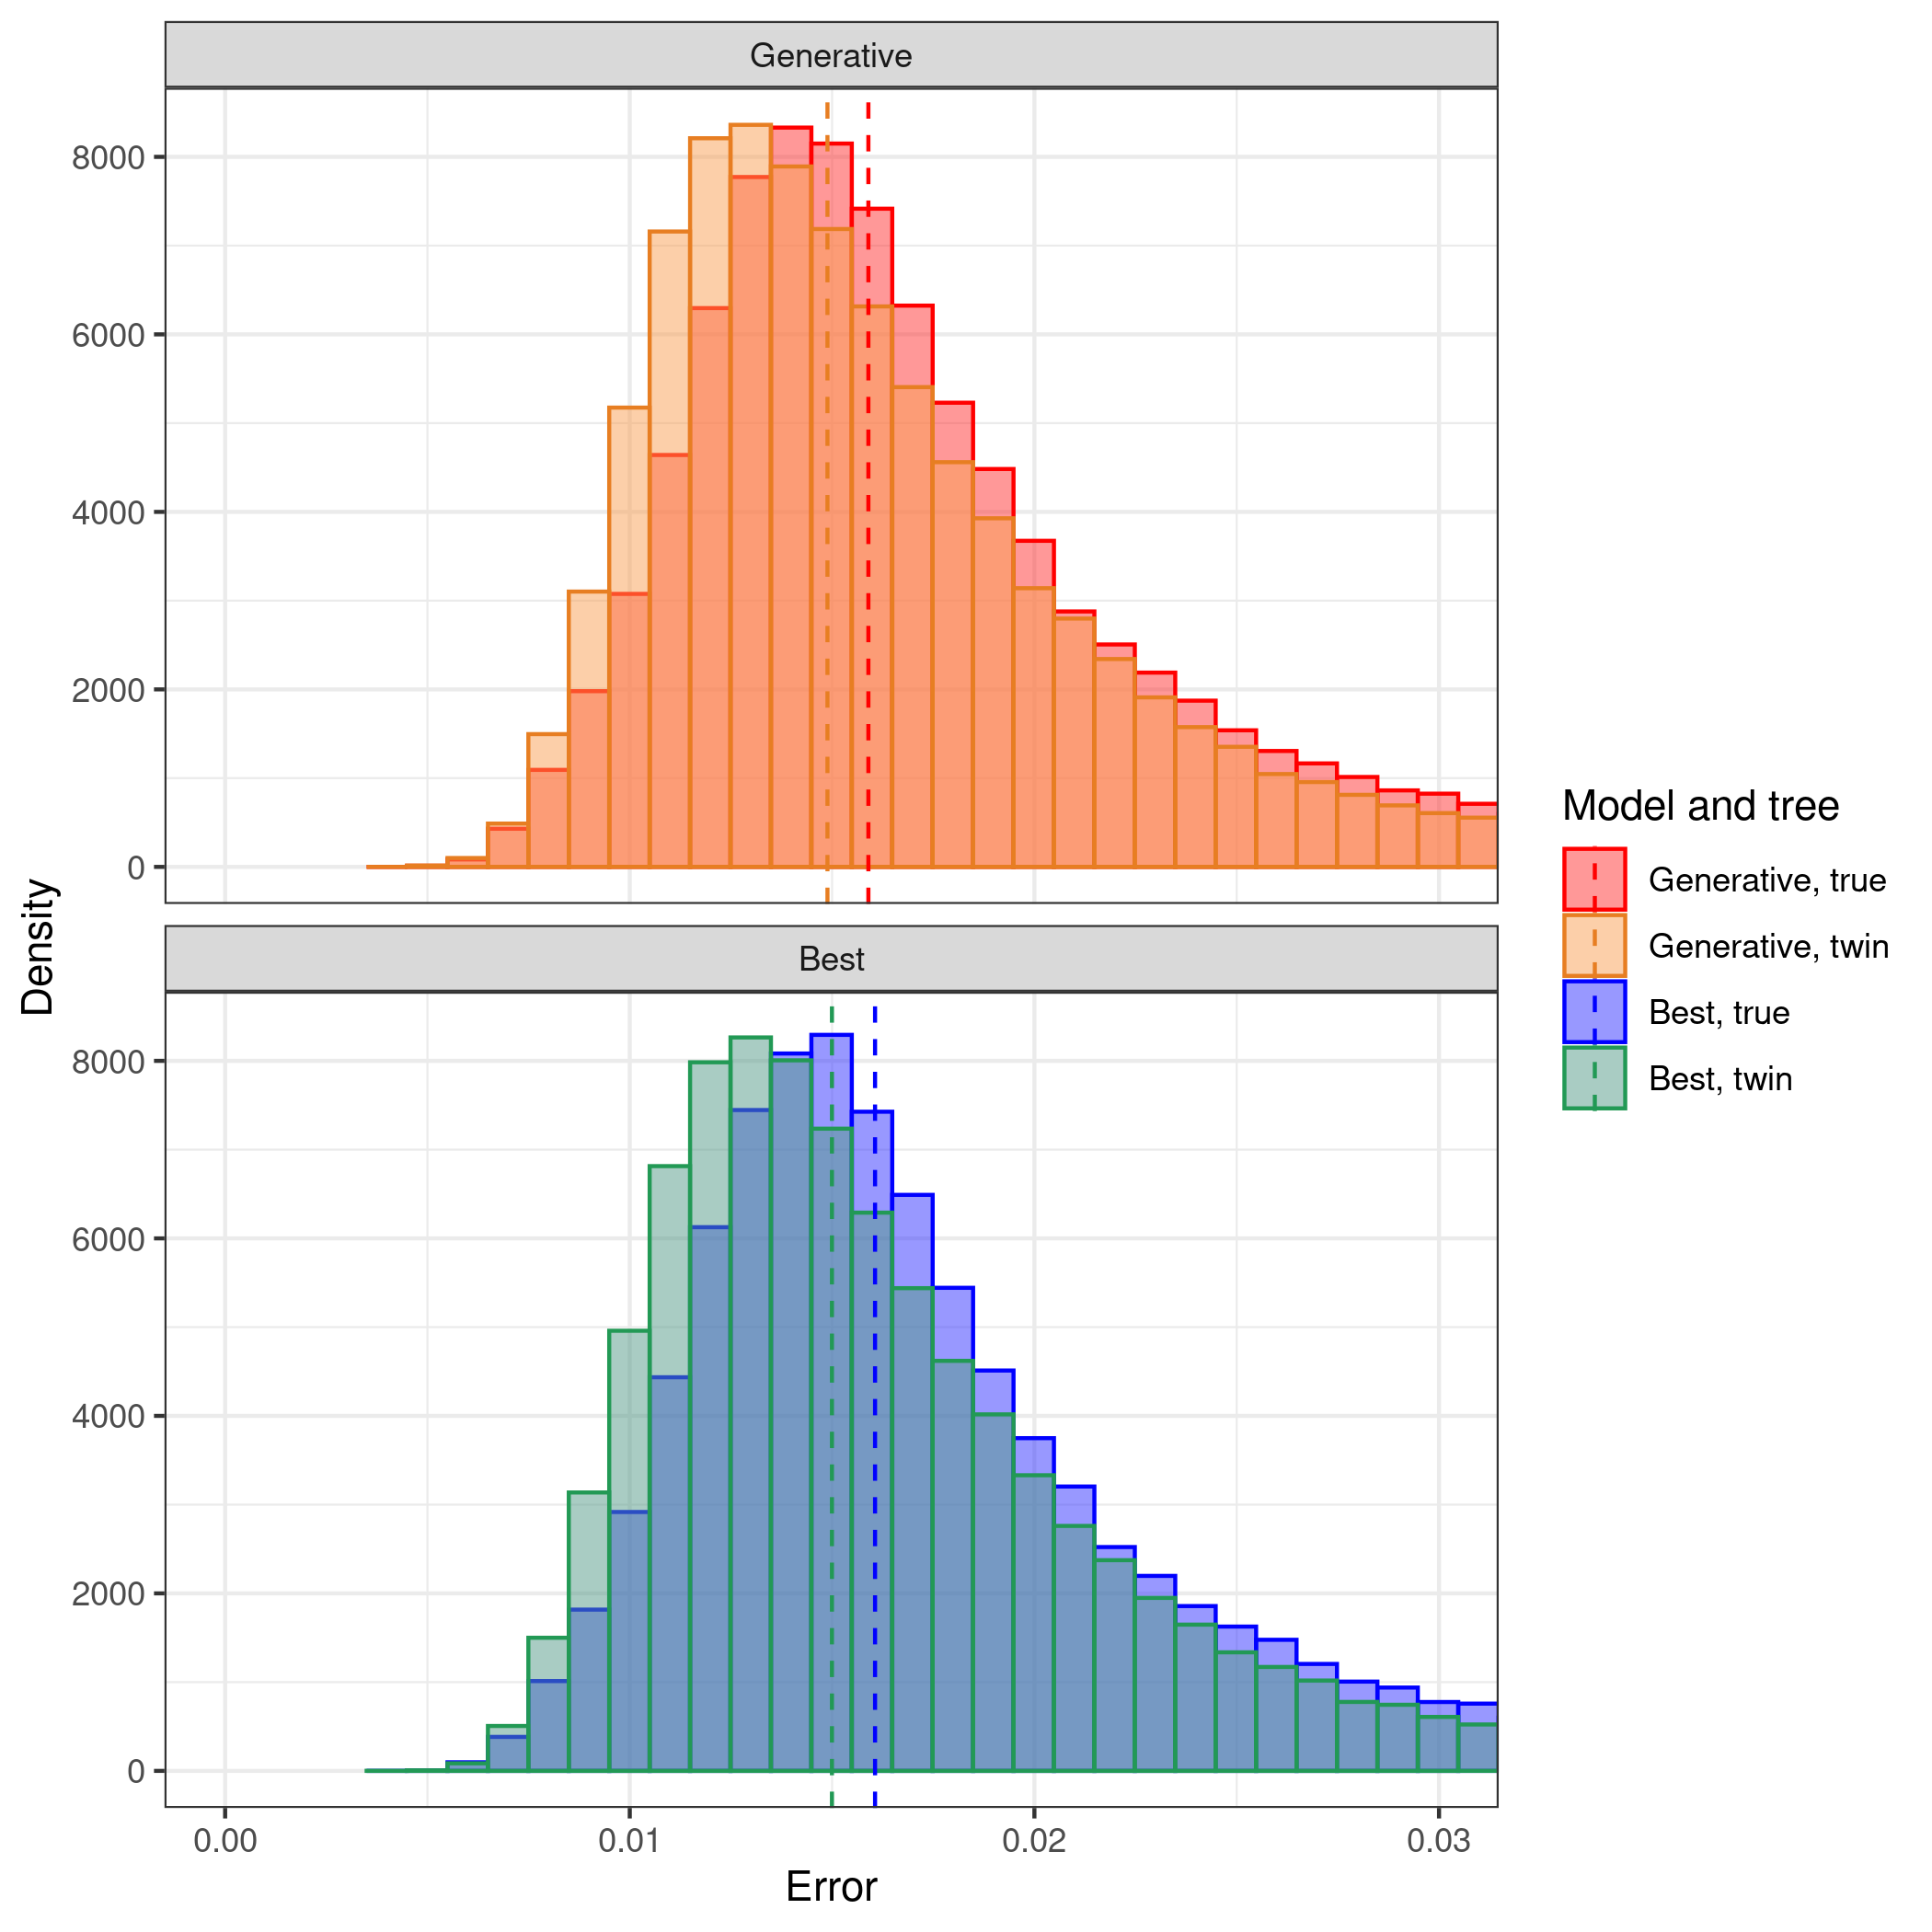
\includegraphics[width=\textwidth]{pirouette_example_23/errors_low.png}
  \caption{Aggregate error distributions for a distribution of trees, where the true trees are DD with low likelihood.}
\end{figure}

\begin{figure}[H]
  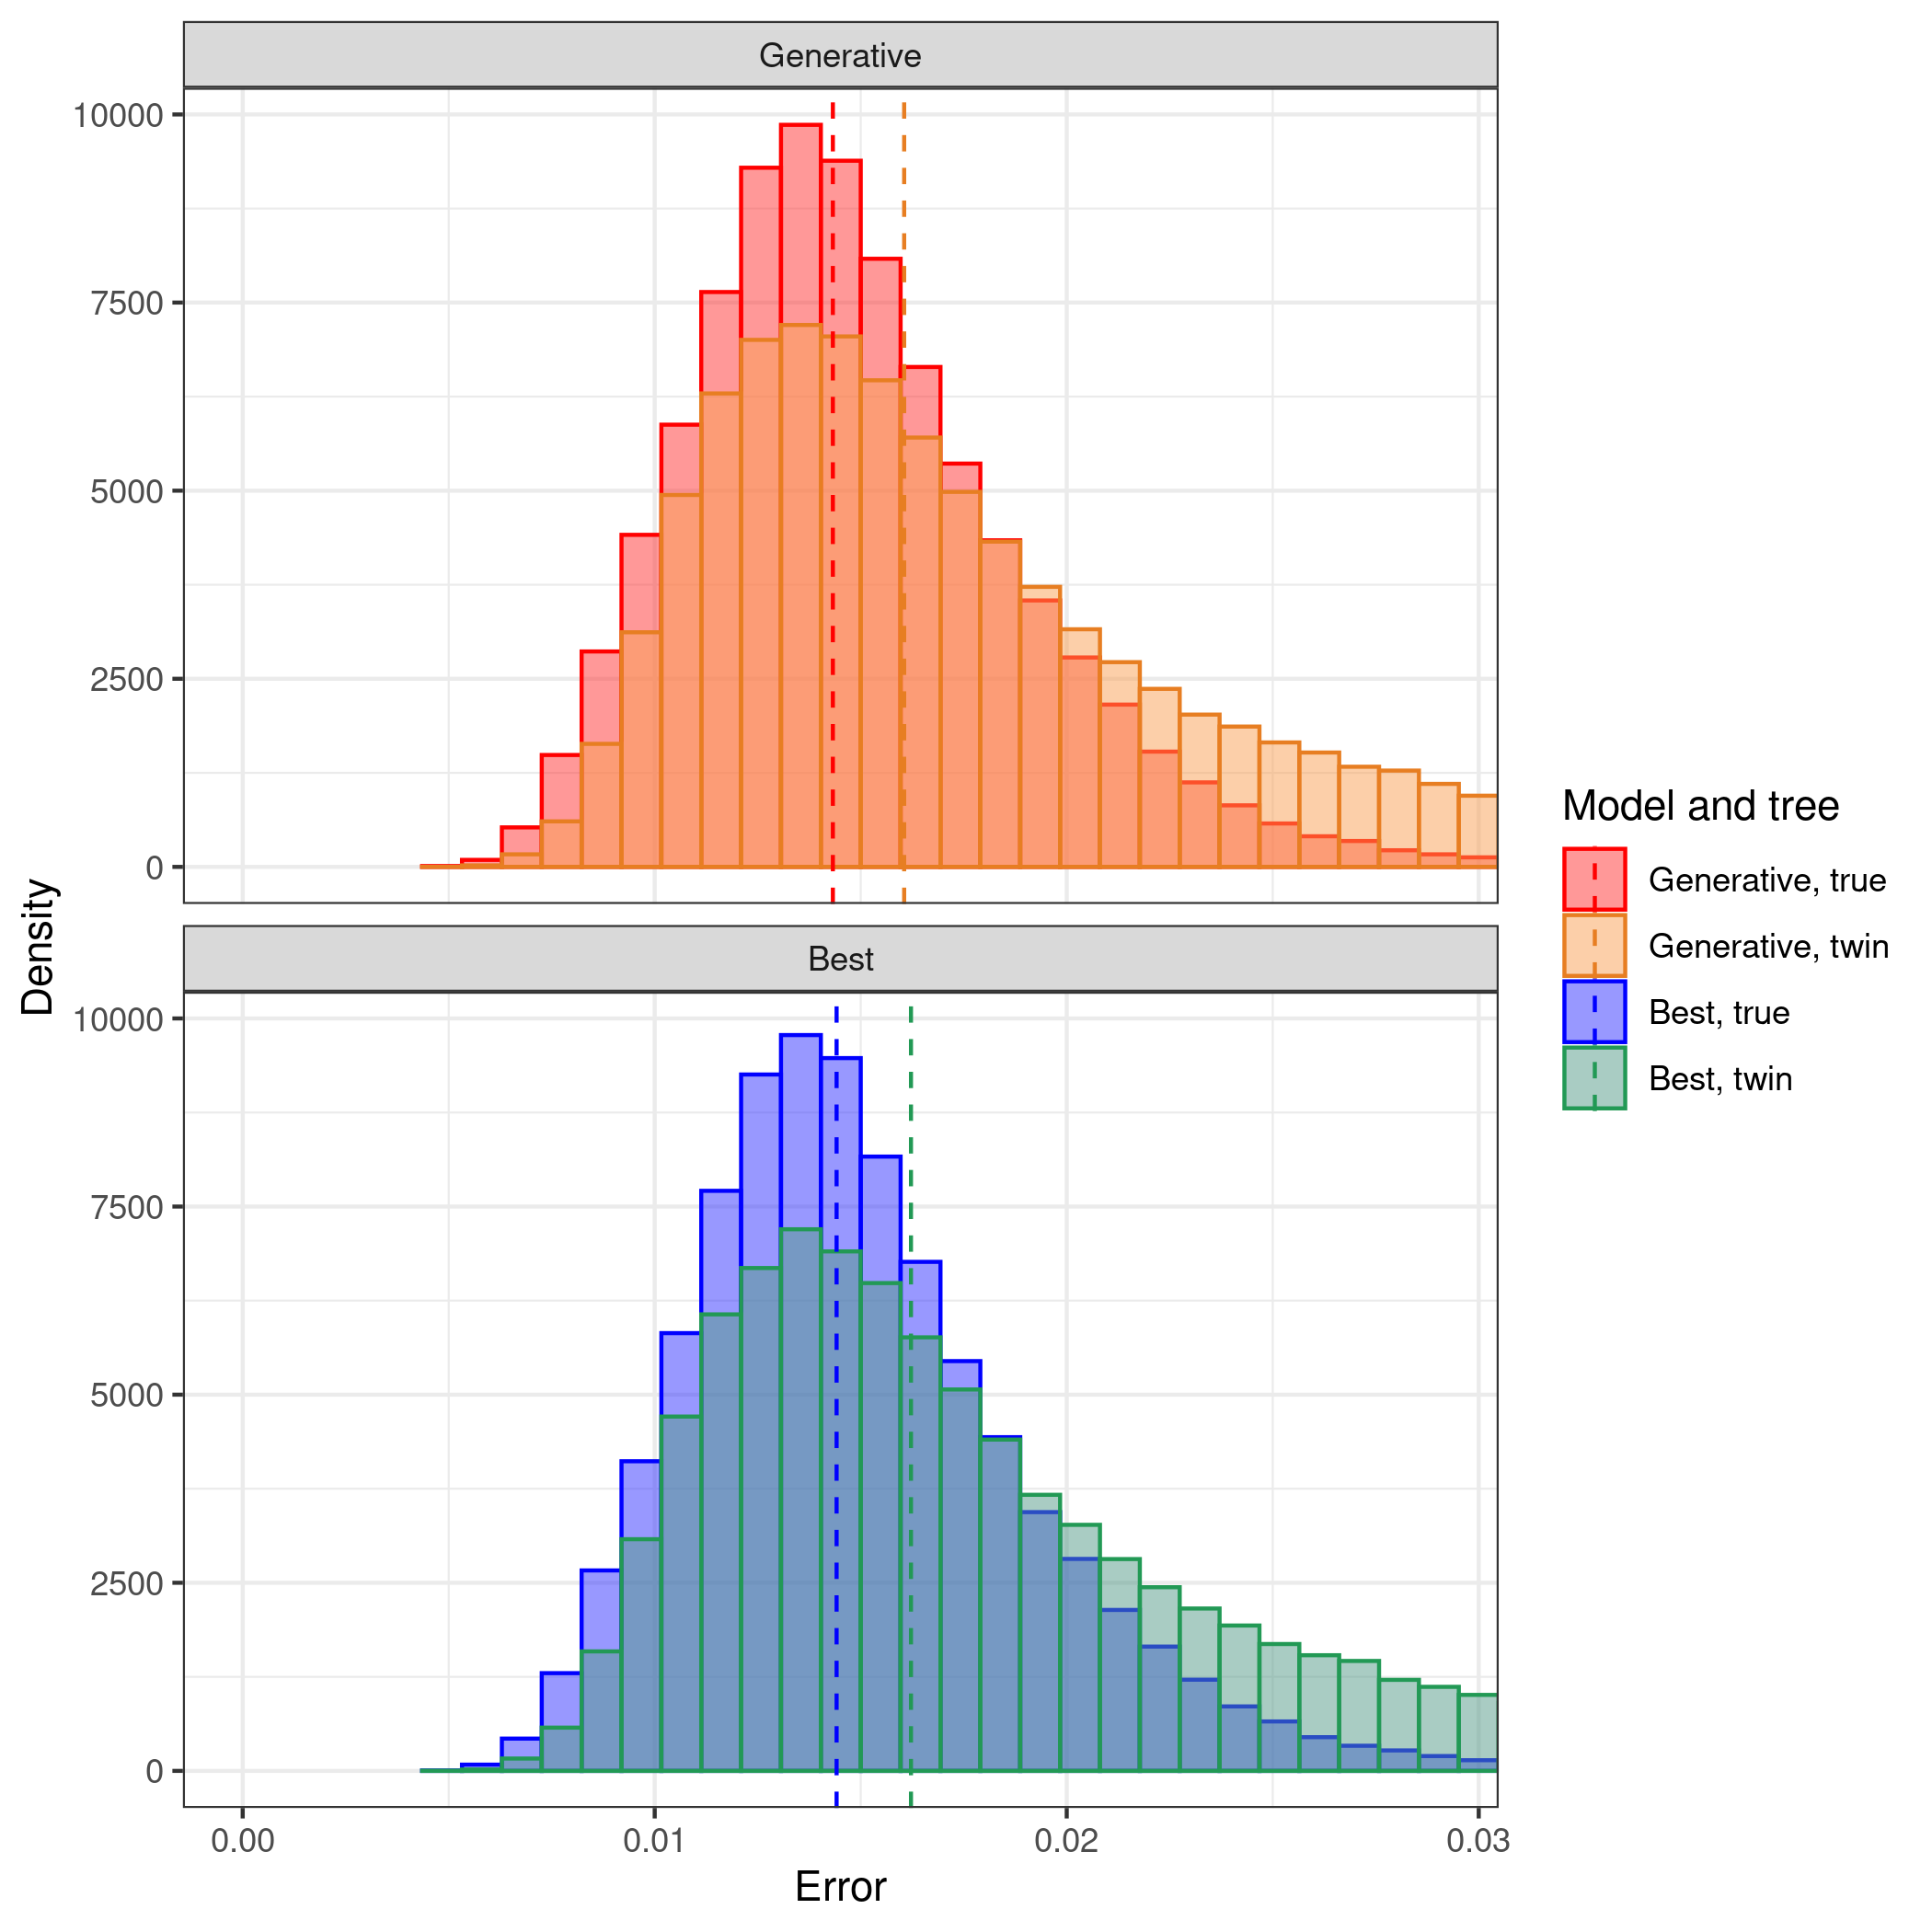
\includegraphics[width=\textwidth]{pirouette_example_23/errors_mid.png}
  \caption{Aggregate error distributions for a distribution of trees, where the true trees are DD with median likelihood.}
\end{figure}

\begin{figure}[H]
  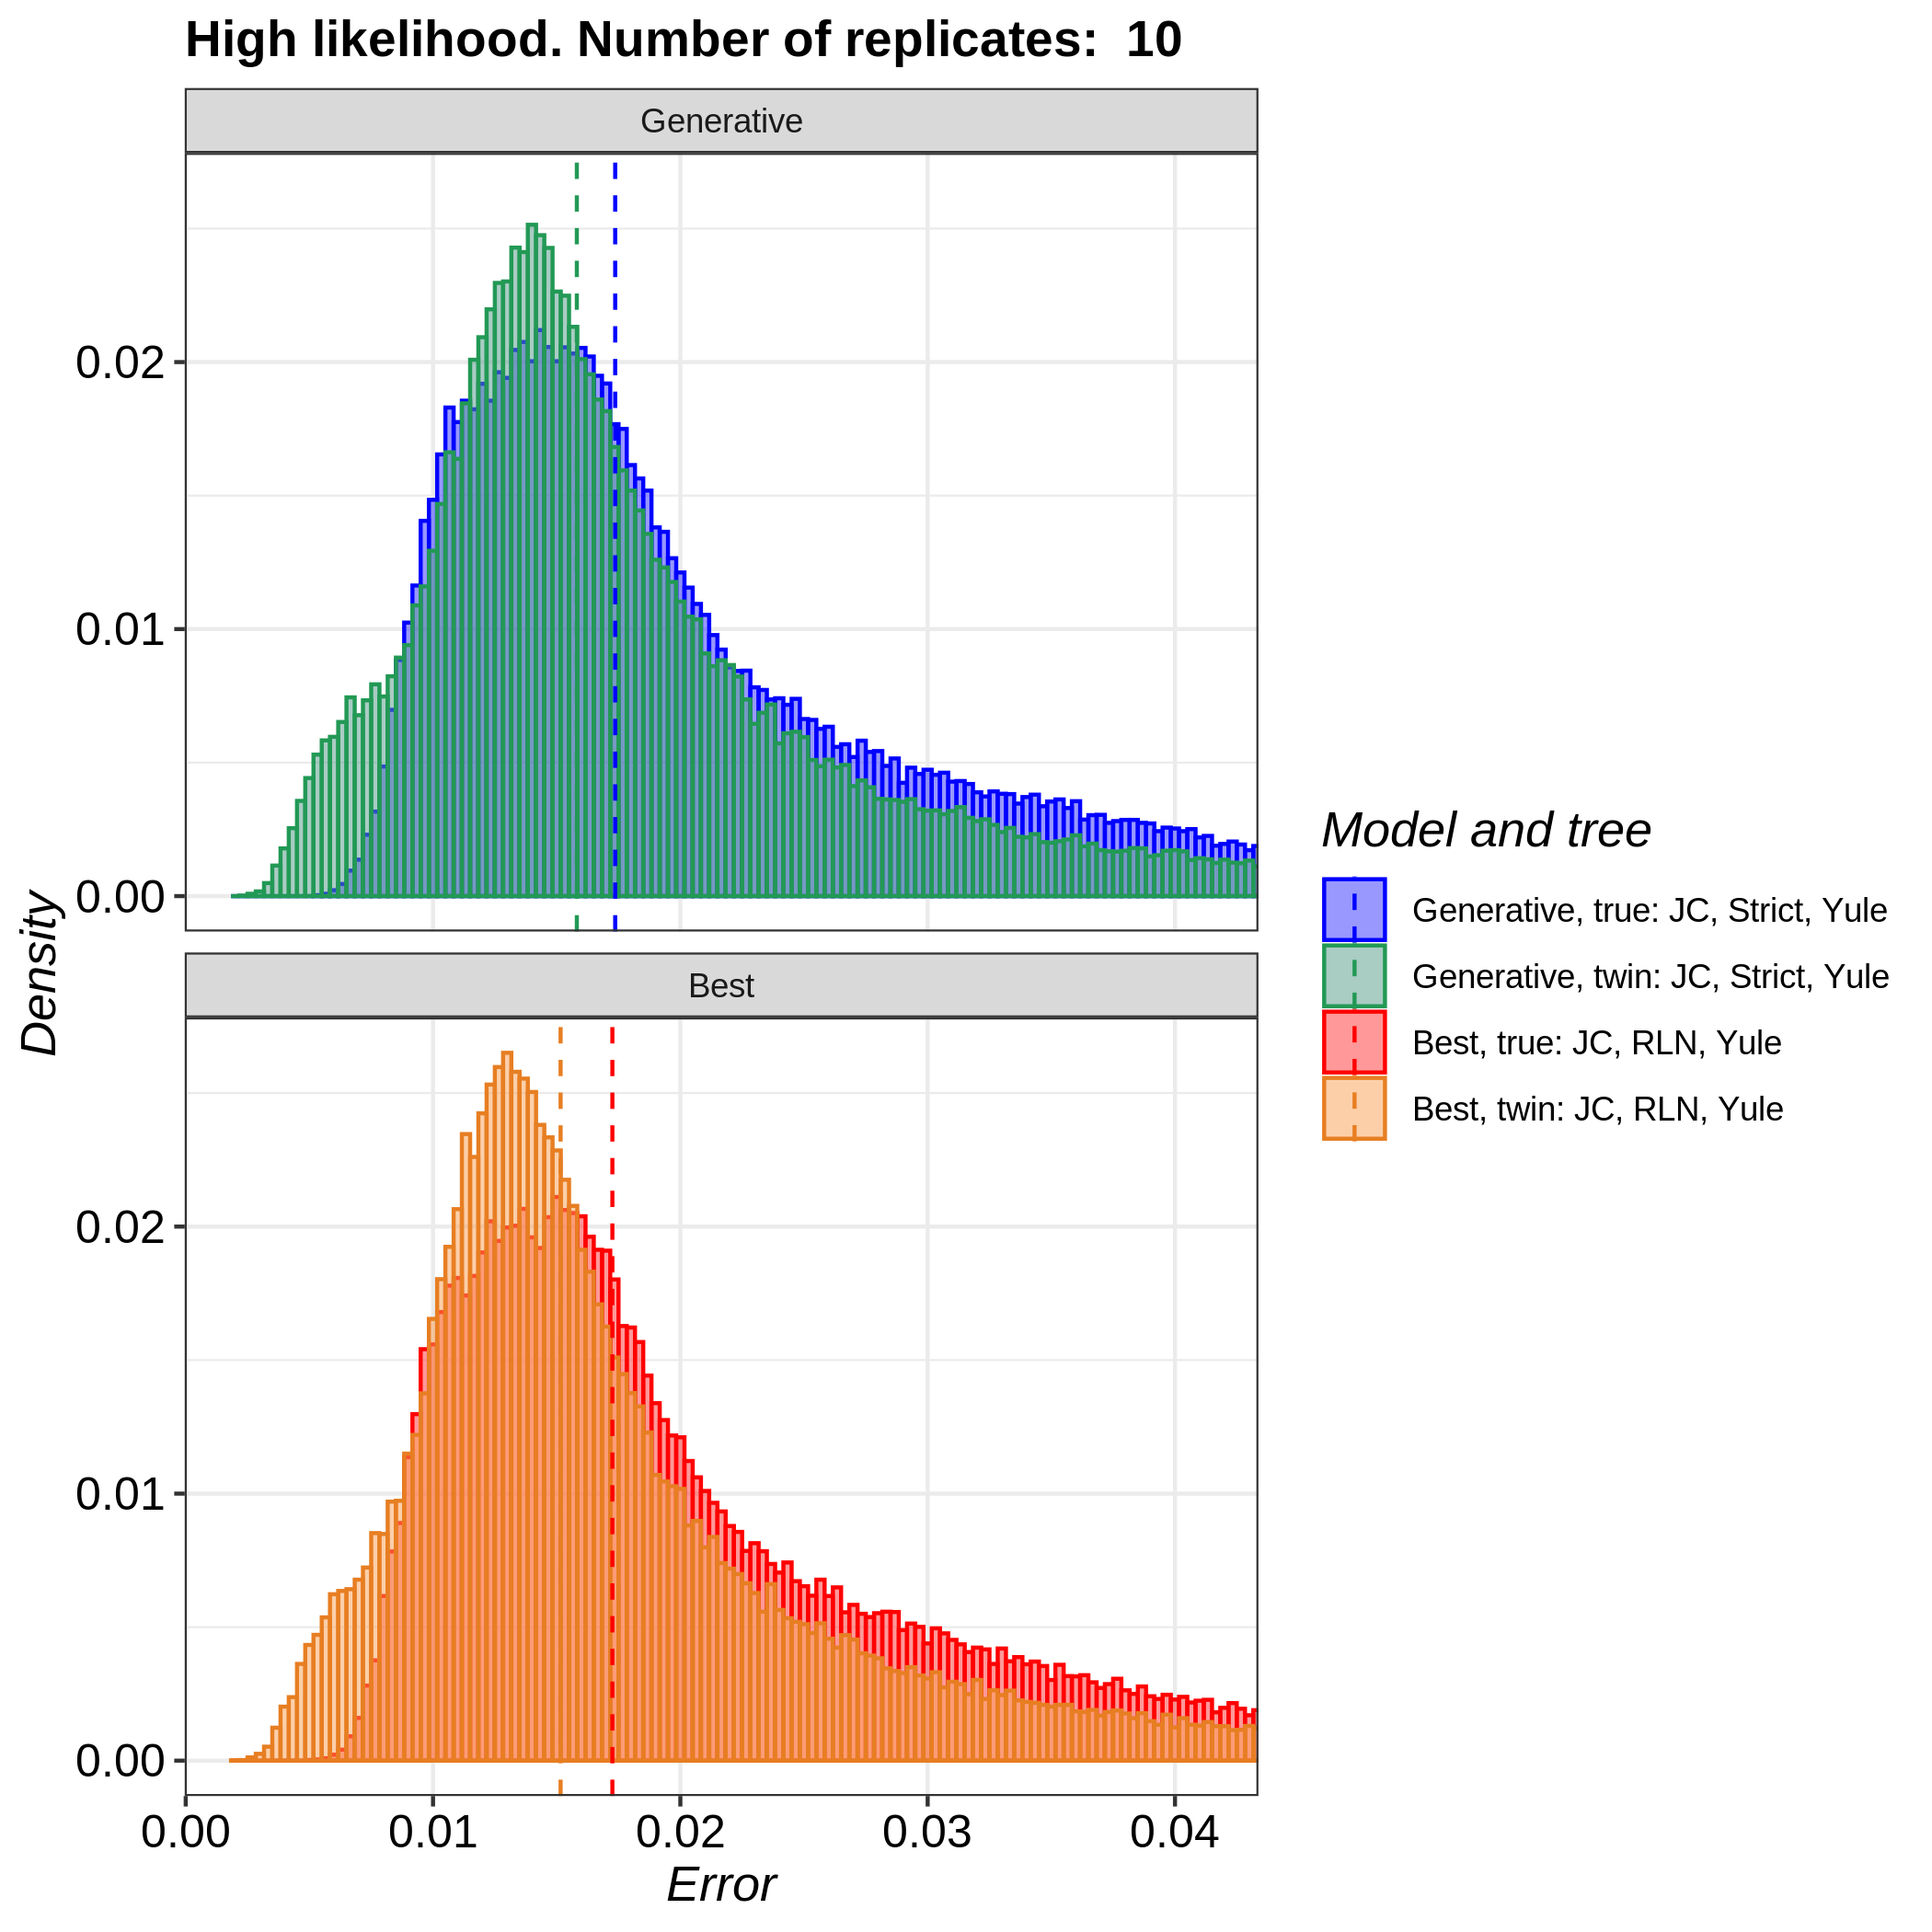
\includegraphics[width=\textwidth]{pirouette_example_23/errors_high.png}
  \caption{Aggregate error distributions for a distribution of trees, where the true trees are DD with high likelihood.}
\end{figure}

%%%%%%%%%%%%%%%%%%%%%%%%%%%%%%%%%%%%%%%%%%%%%%%%%%%%%%%%%%%%%%%%%%%%%%%%%%%%%%%%
\subsection{The effect of equal or equalized mutation rate in the twin alignment}
\label{subsec:different_n_mutations}
%%%%%%%%%%%%%%%%%%%%%%%%%%%%%%%%%%%%%%%%%%%%%%%%%%%%%%%%%%%%%%%%%%%%%%%%%%%%%%%%
  
The main example uses a twin alignment that has the same number
of mutations (as measured from the ancestral sequence) as the true alignment. Here, we show the same results, with the difference that
the twin alignment uses the same mutation rate, yet is not guaranteed
to have the same number of mutations. Any difference in the error distributions can therefore also stem from a difference in the amount of information contained in the alignments.

The code to reproduce this figure can be found at  
\url{https://github.com/richelbilderbeek/pirouette_example_18} and
\url{https://github.com/richelbilderbeek/pirouette_example_28}.

\begin{figure}[H]
  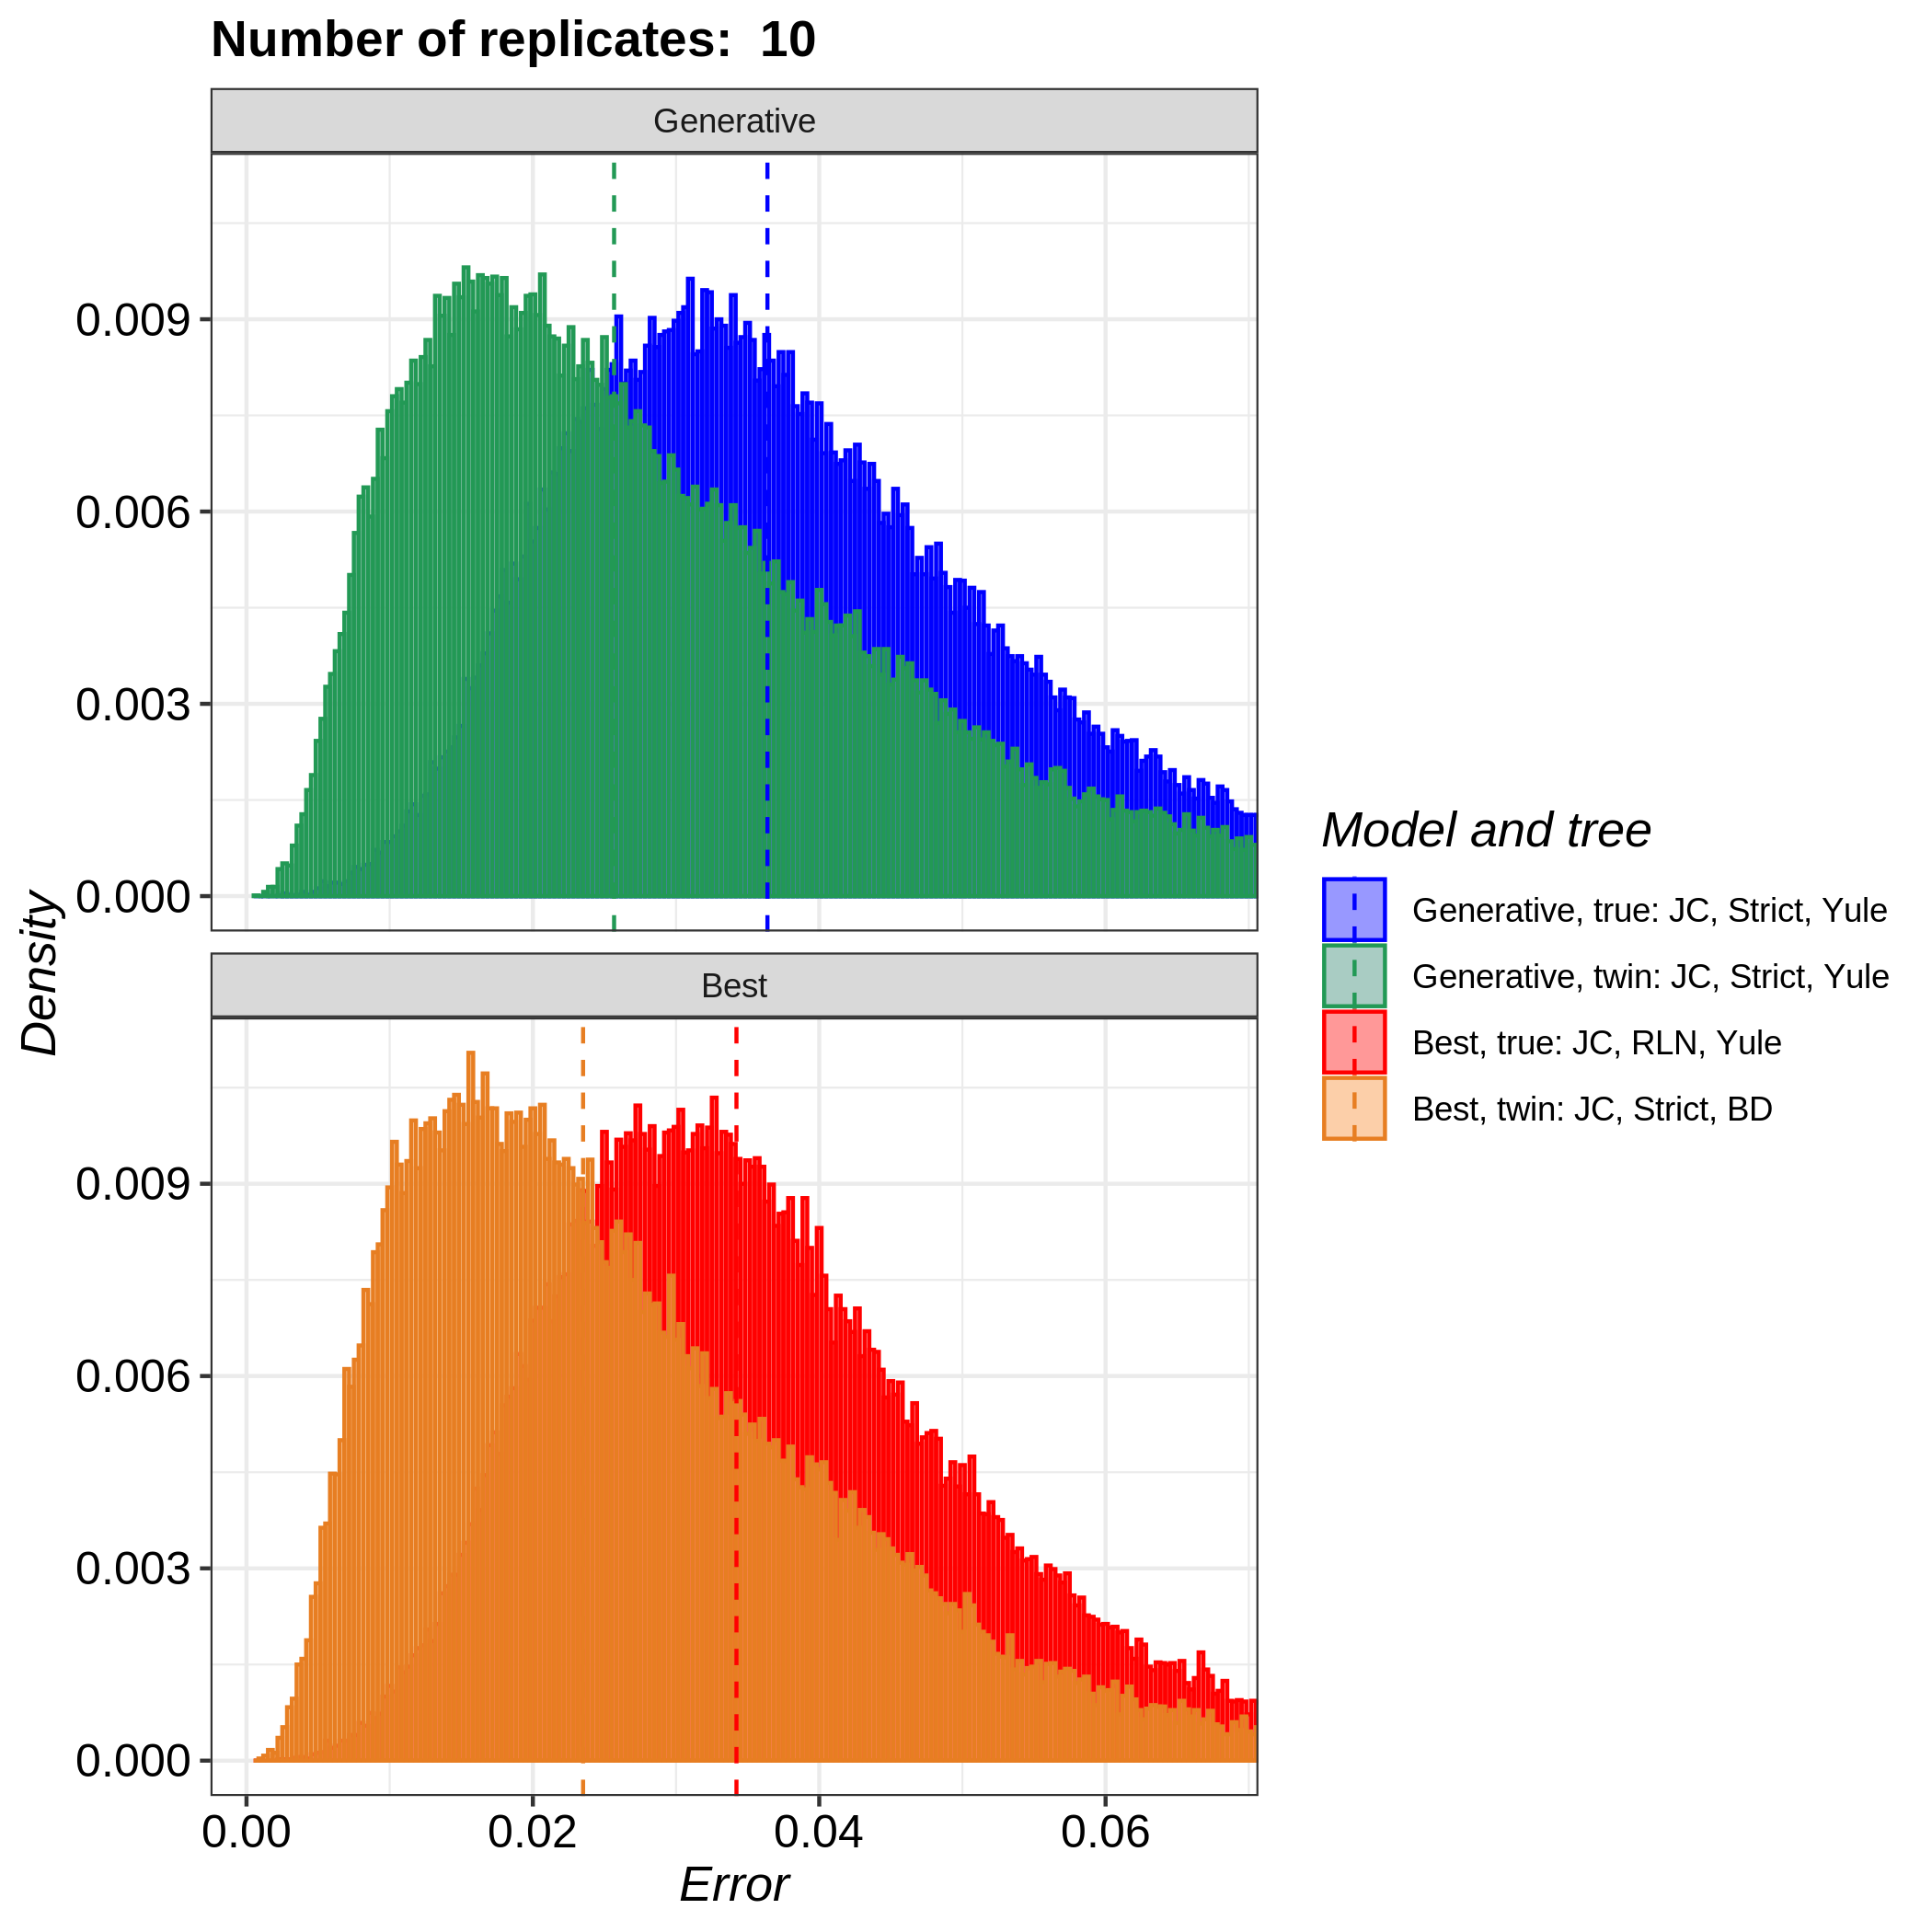
\includegraphics[width=\textwidth]{pirouette_example_18/errors.png}
  \caption{Aggregate error distributions similar to Fig. \ref{fig:replicate_trees}, but here the number of mutations is not imposed to be the same between true and twin alignment. Instead we just use an equal mutation rate. This took 10 hours to compute.}
\end{figure}

\clearpage

%%%%%%%%%%%%%%%%%%%%%%%%%%%%%%%%%%%%%%%%%%%%%%%%%%%%%%%%%%%%%%%%%%%%%%%%%%%%%%%%
\subsection{The effect of mutation rate}
\label{subsec:mutation_rate}
%%%%%%%%%%%%%%%%%%%%%%%%%%%%%%%%%%%%%%%%%%%%%%%%%%%%%%%%%%%%%%%%%%%%%%%%%%%%%%%%

The main example uses a mutation rate such that all nucleotides,
on average, mutate once over the history going from the
ancestral sequence at the crown to the alignments at the tips.
This value equals `1.0 / crown age`.
In this way, the alignment is expected to contain the maximum
amount of information.

Here, we show the same results for different mutation rates.

The code to reproduce this figure can be found at  
\url{https://github.com/richelbilderbeek/pirouette_example_35} (0.25 / crown age),
\url{https://github.com/richelbilderbeek/pirouette_example_36} (0.50 / crown age),
\url{https://github.com/richelbilderbeek/pirouette_example_37} (0.75 / crown age),
\url{https://github.com/richelbilderbeek/pirouette_example_28} (1.00 / crown age, example reported in \ref{subsec:distribution}, see Fig. \ref{fig:replicate_trees}),
\url{https://github.com/richelbilderbeek/pirouette_example_38} (1.25 / crown age),
\url{https://github.com/richelbilderbeek/pirouette_example_39} (1.50 / crown age),
\url{https://github.com/richelbilderbeek/pirouette_example_40} (2.00 / crown age),

\begin{figure}[H]
  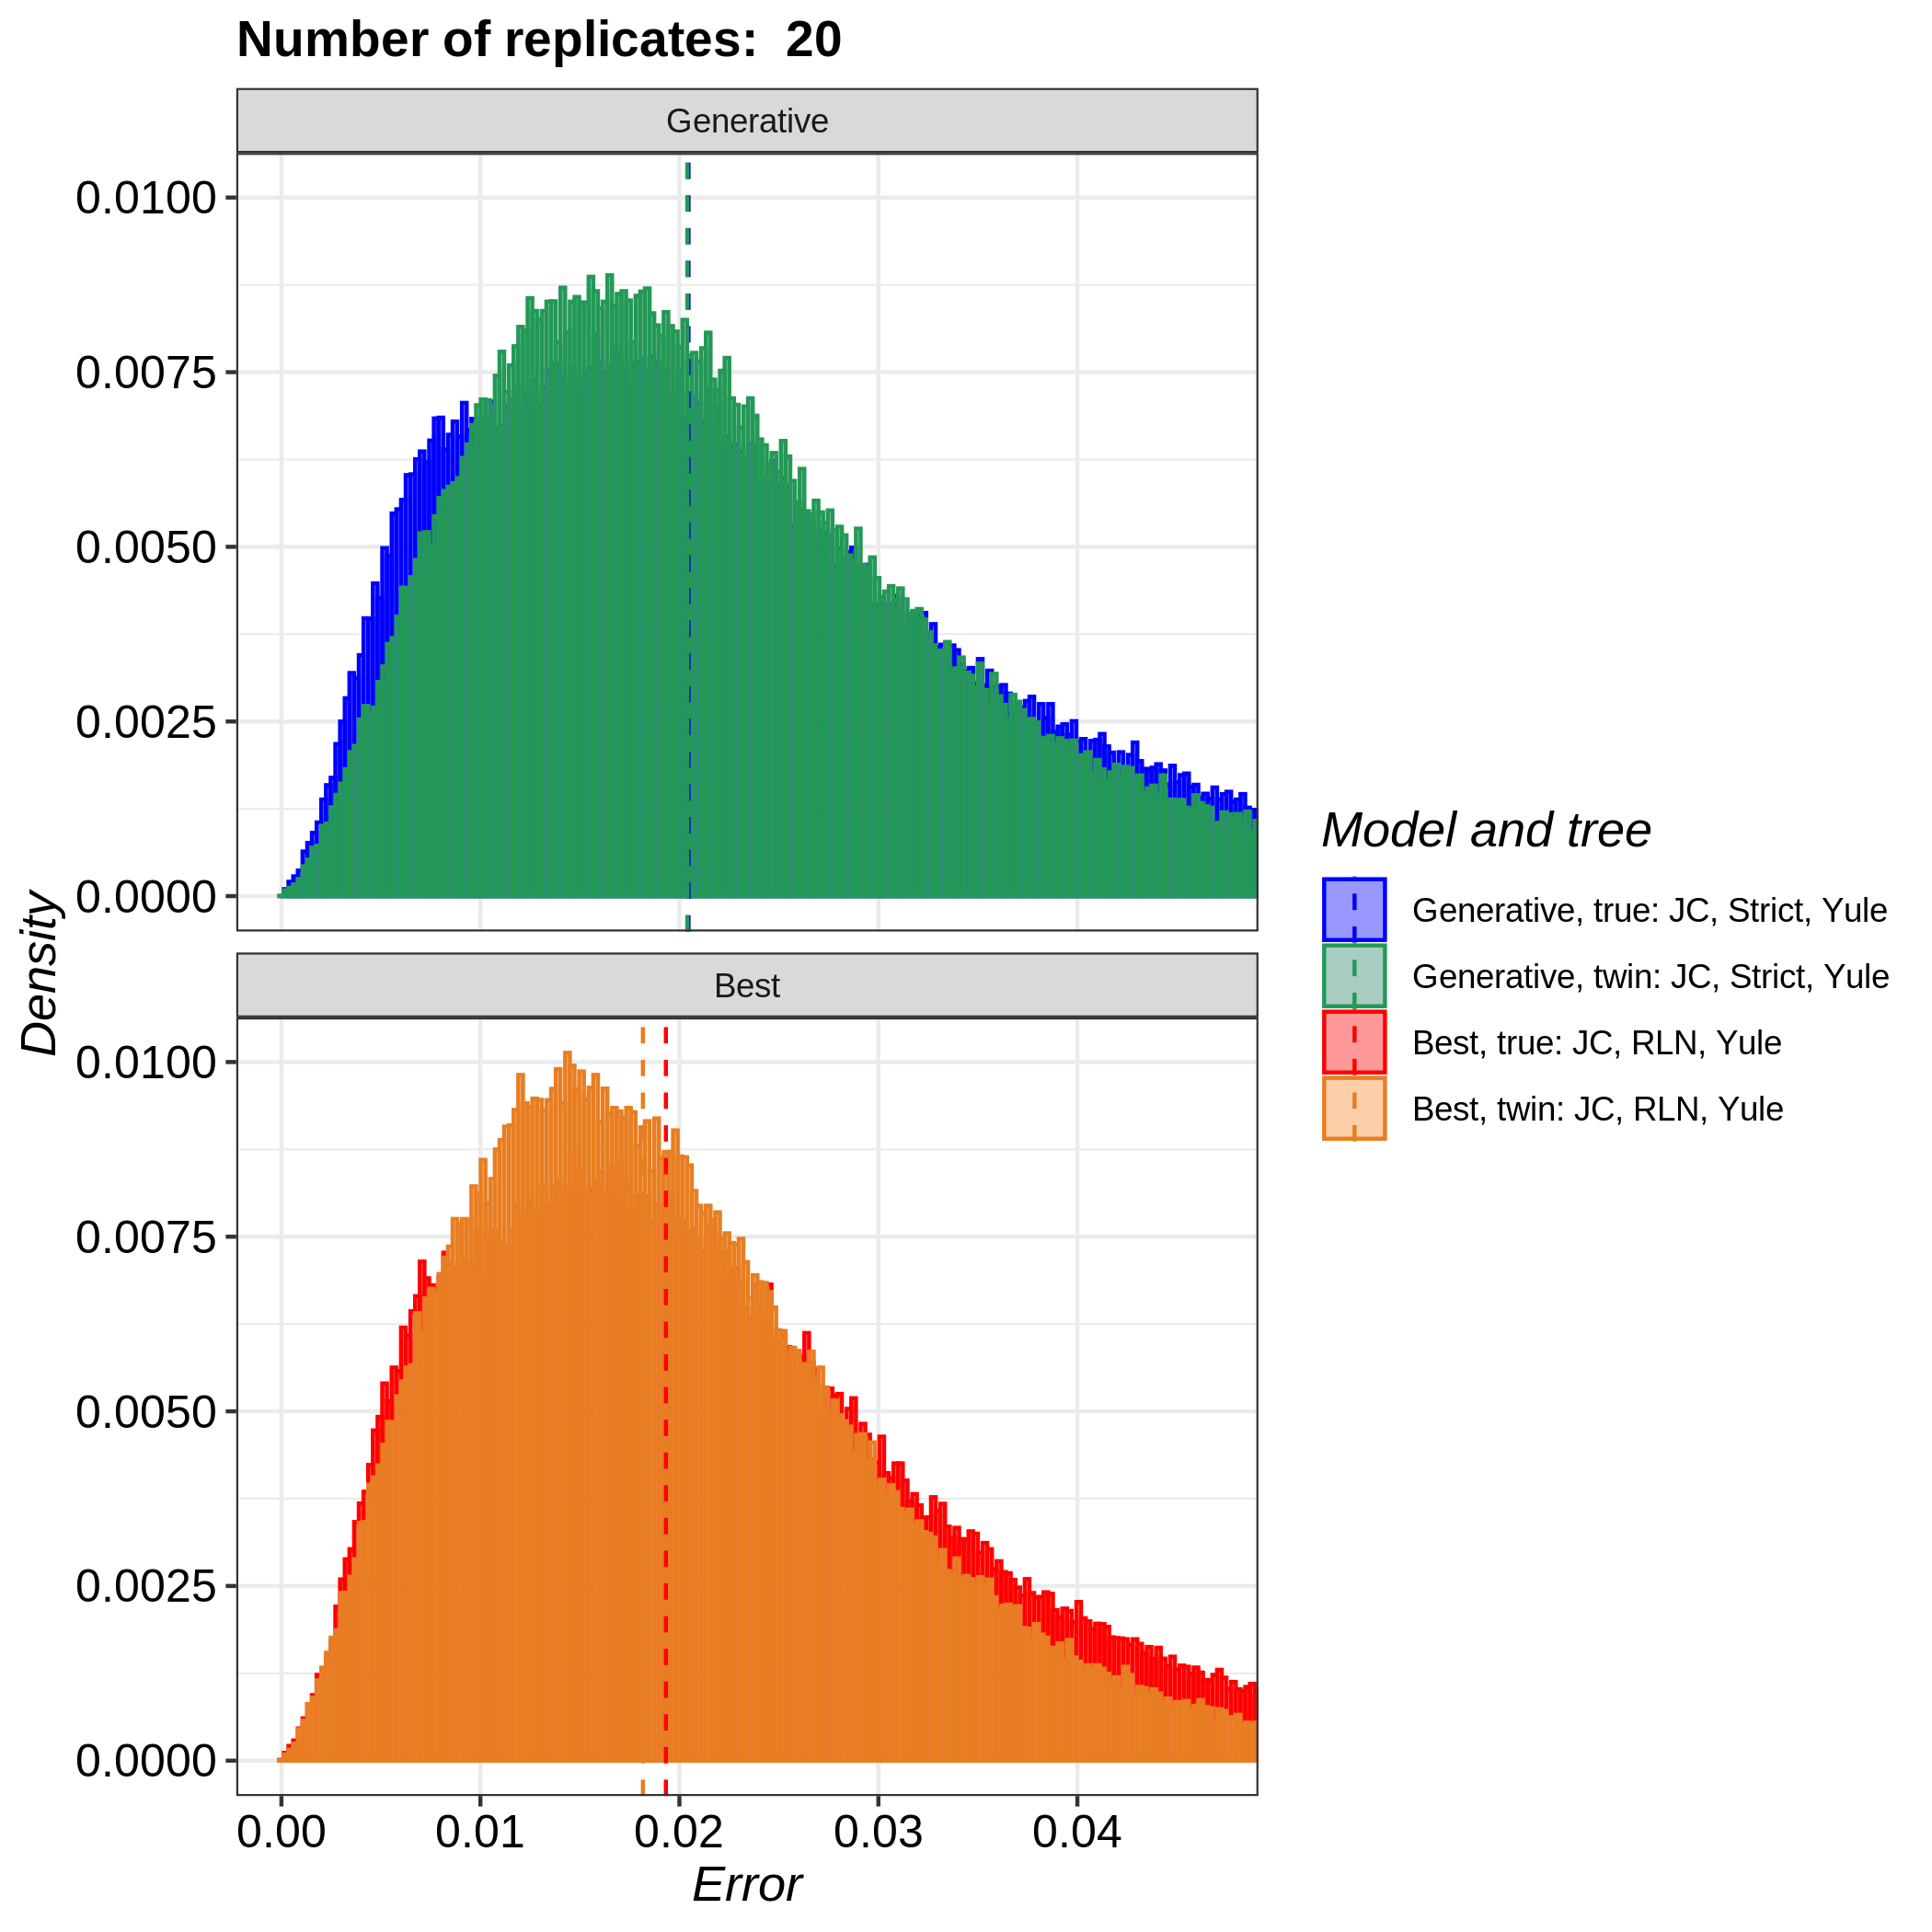
\includegraphics[width=\textwidth]{pirouette_example_35/errors.png}
  \caption{Aggregate error distributions for the tree distribution presented in \ref{subsec:distribution} but with a per-nucleotide mutation rate of 0.25 / crown age. This took 11 hours to compute.}
\end{figure}

\begin{figure}[H]
  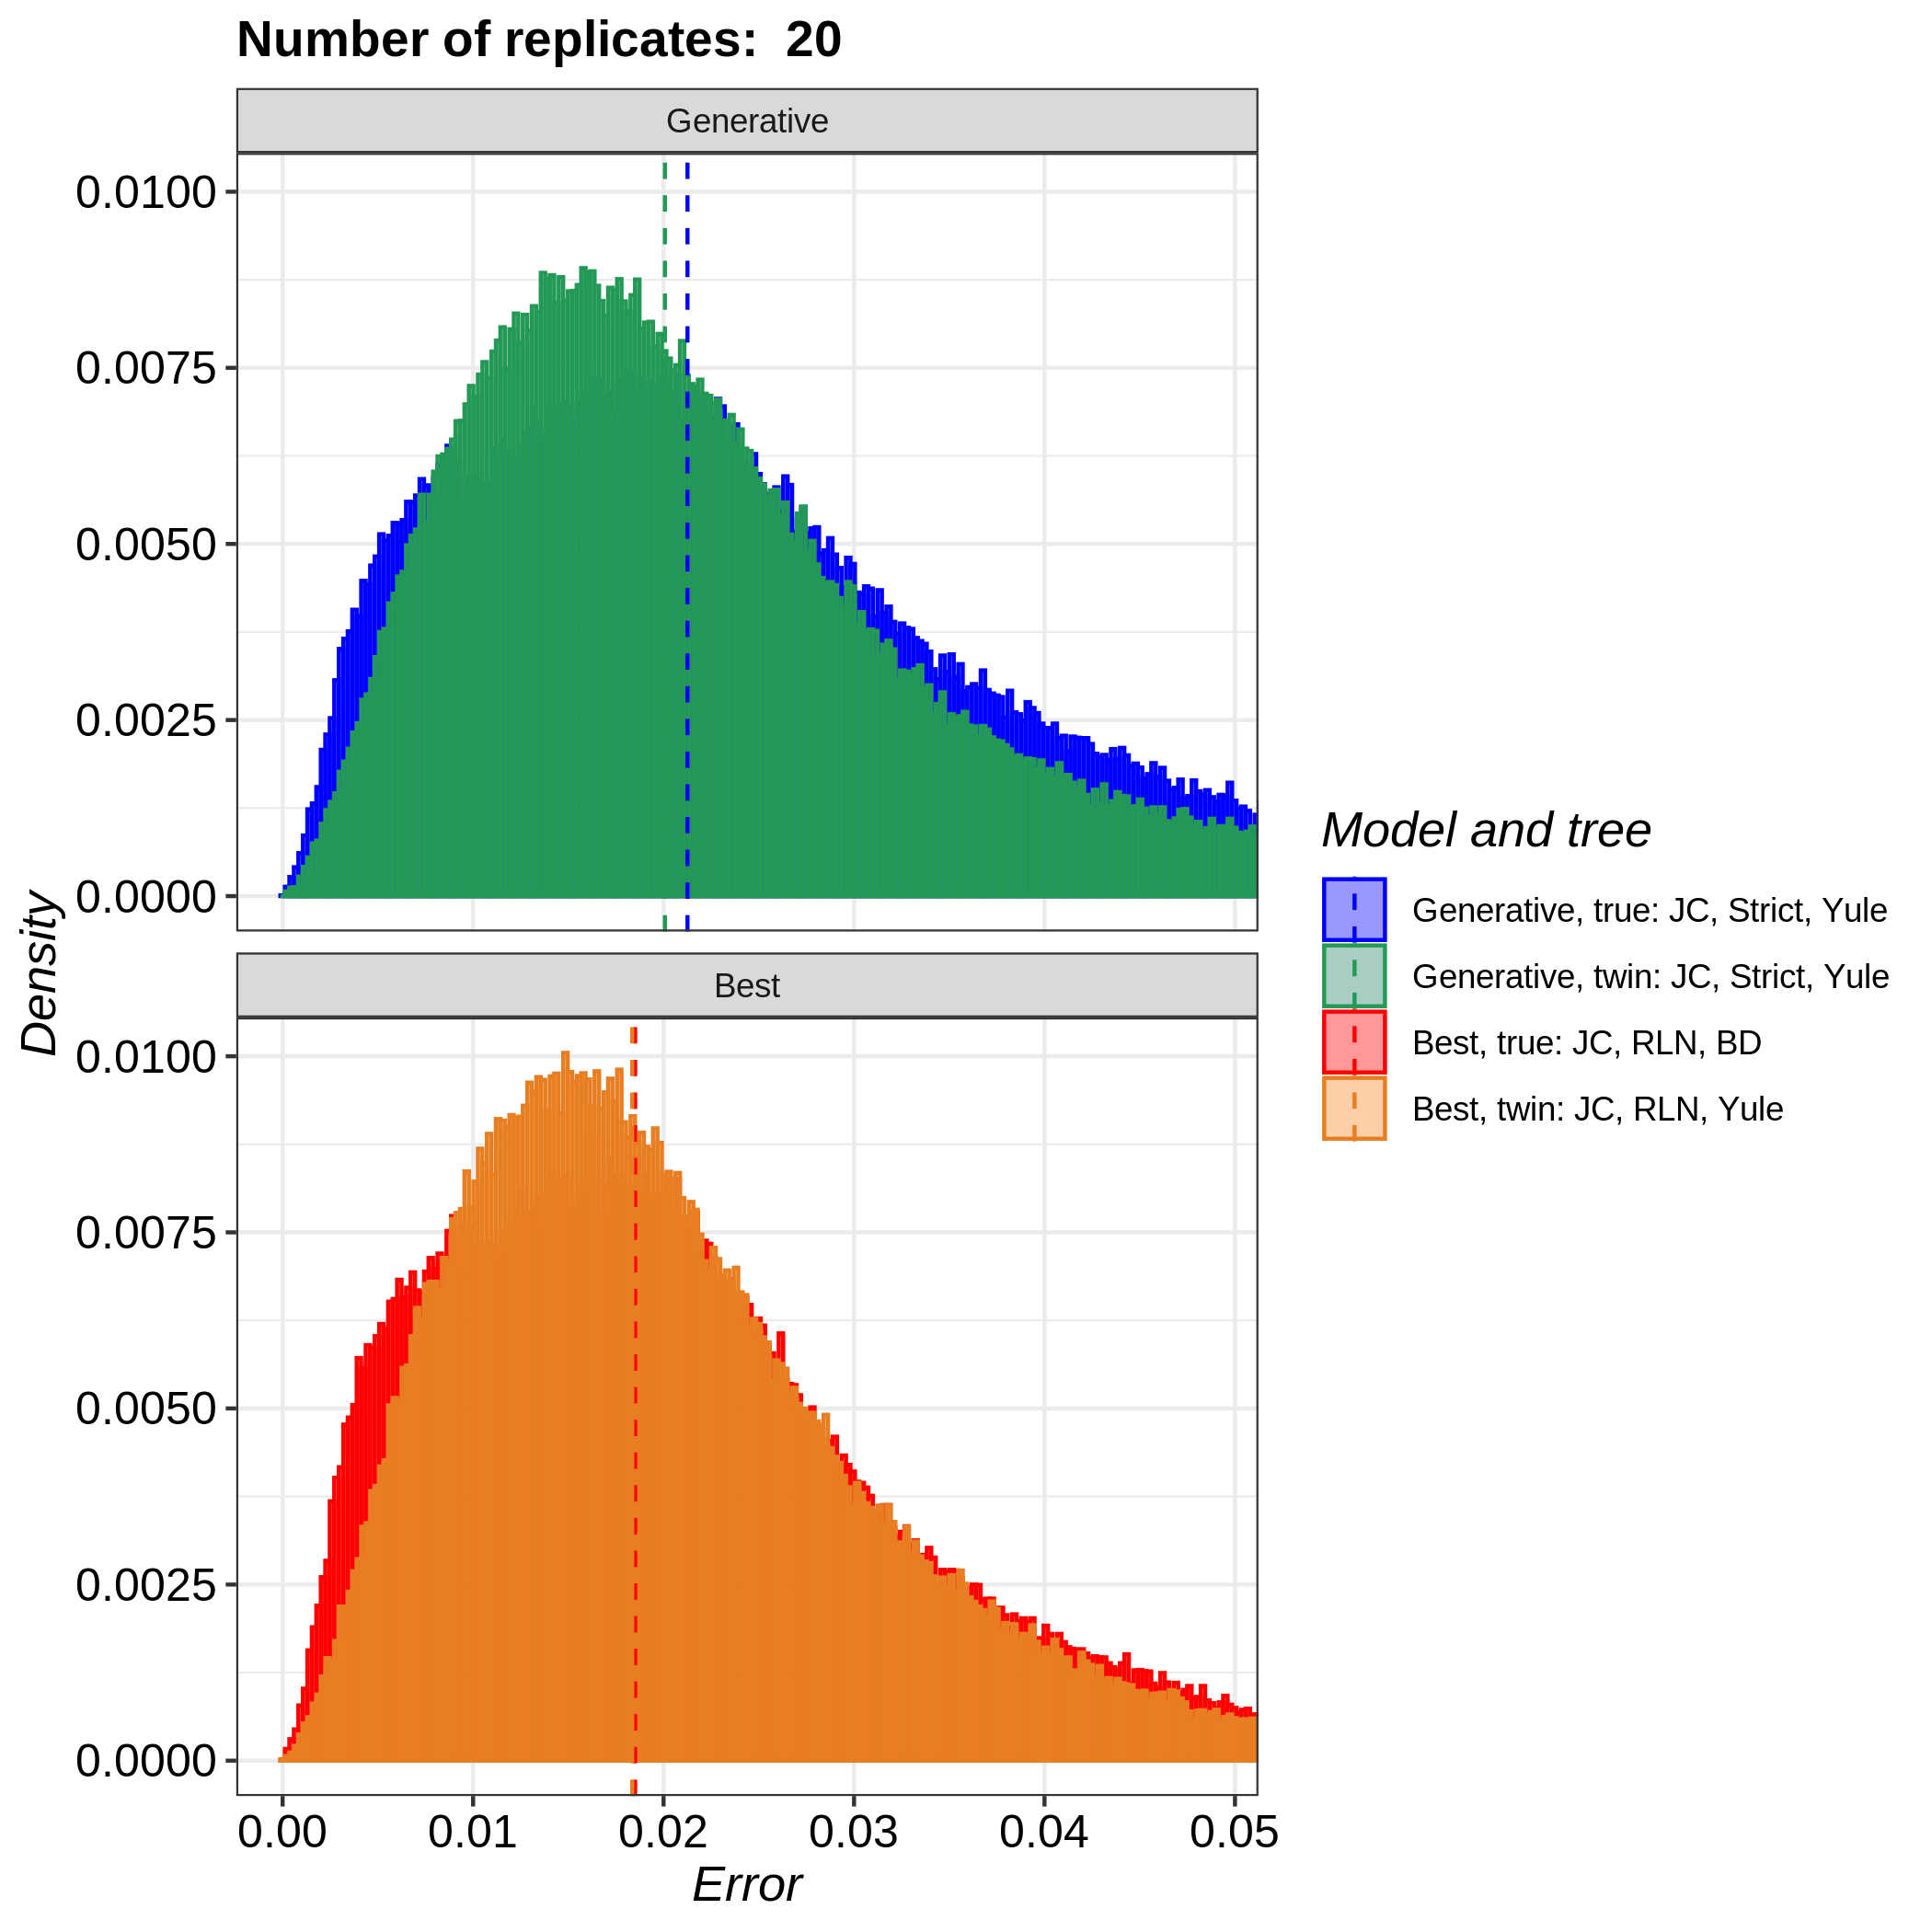
\includegraphics[width=\textwidth]{pirouette_example_36/errors.png}
  \caption{Aggregate error distributions for the tree distribution presented in \ref{subsec:distribution} but with a per-nucleotide mutation rate of 0.50 / crown age. This took 14 hours to compute.}
\end{figure}

\begin{figure}[H]
  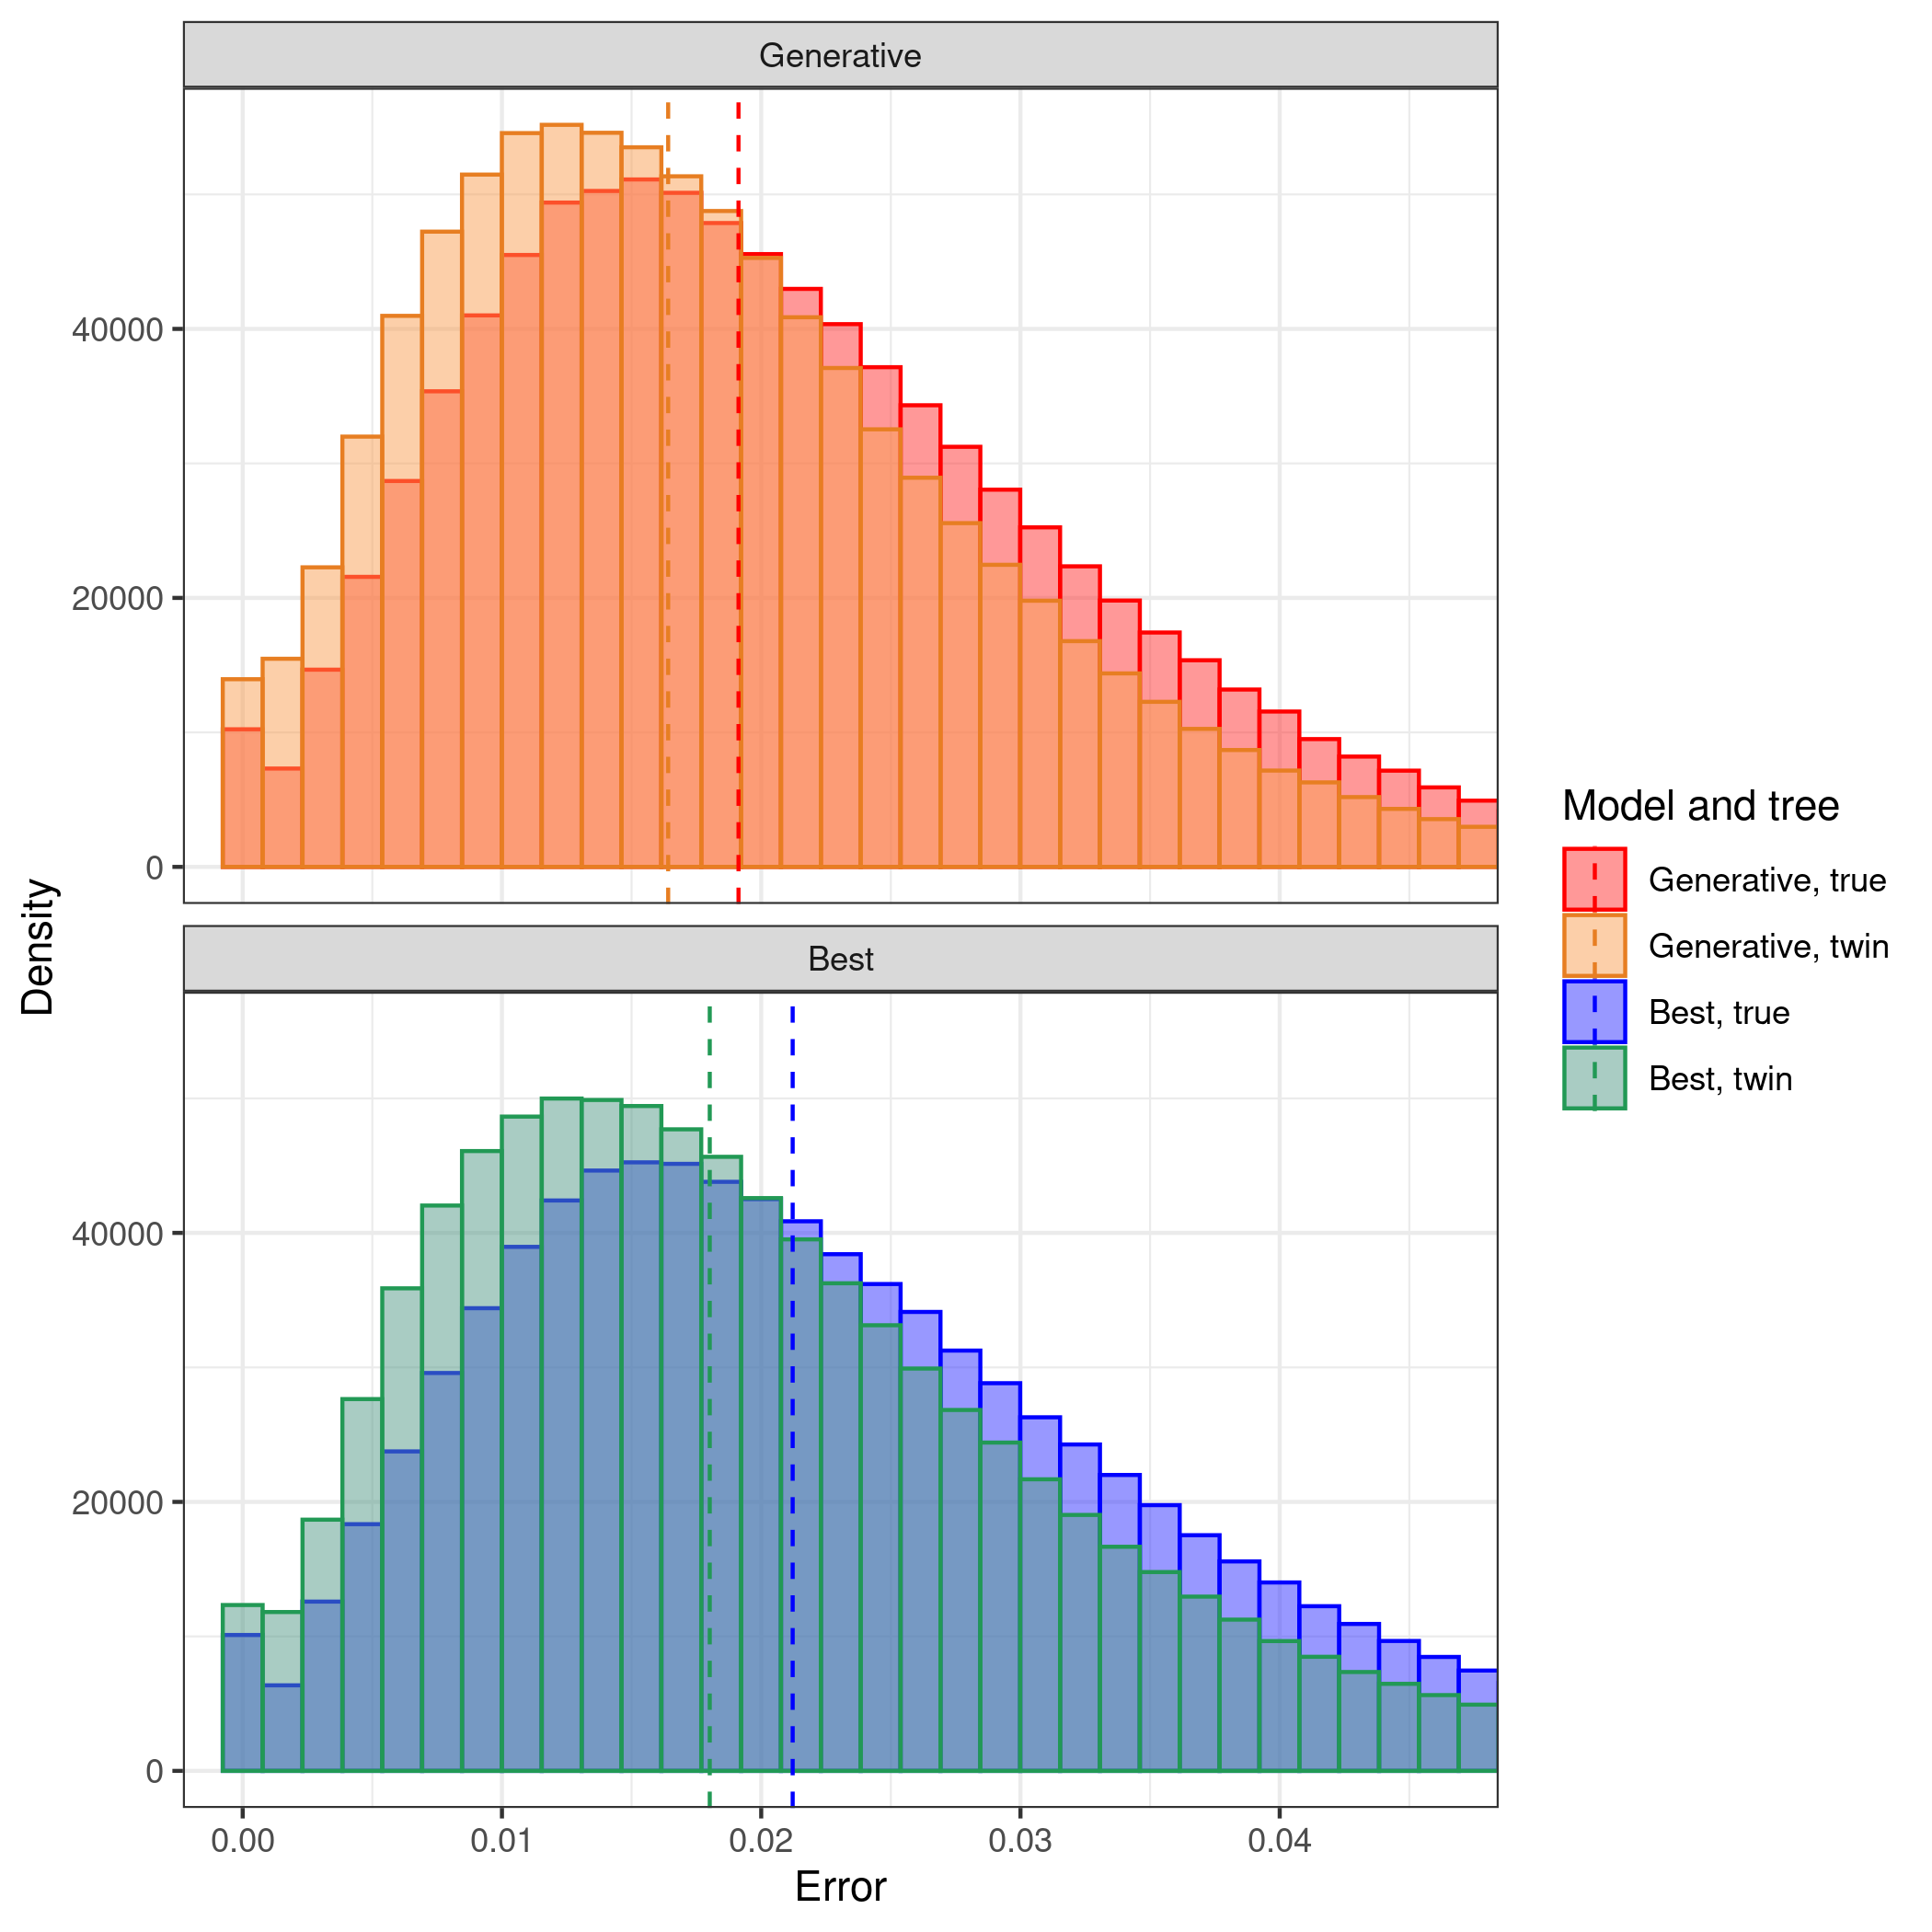
\includegraphics[width=\textwidth]{pirouette_example_37/errors.png}
  \caption{Aggregate error distributions for the tree distribution presented in \ref{subsec:distribution} but with a per-nucleotide mutation rate of 0.75 / crown age. This took 16 hours to compute.}
\end{figure}

\begin{figure}[H]
  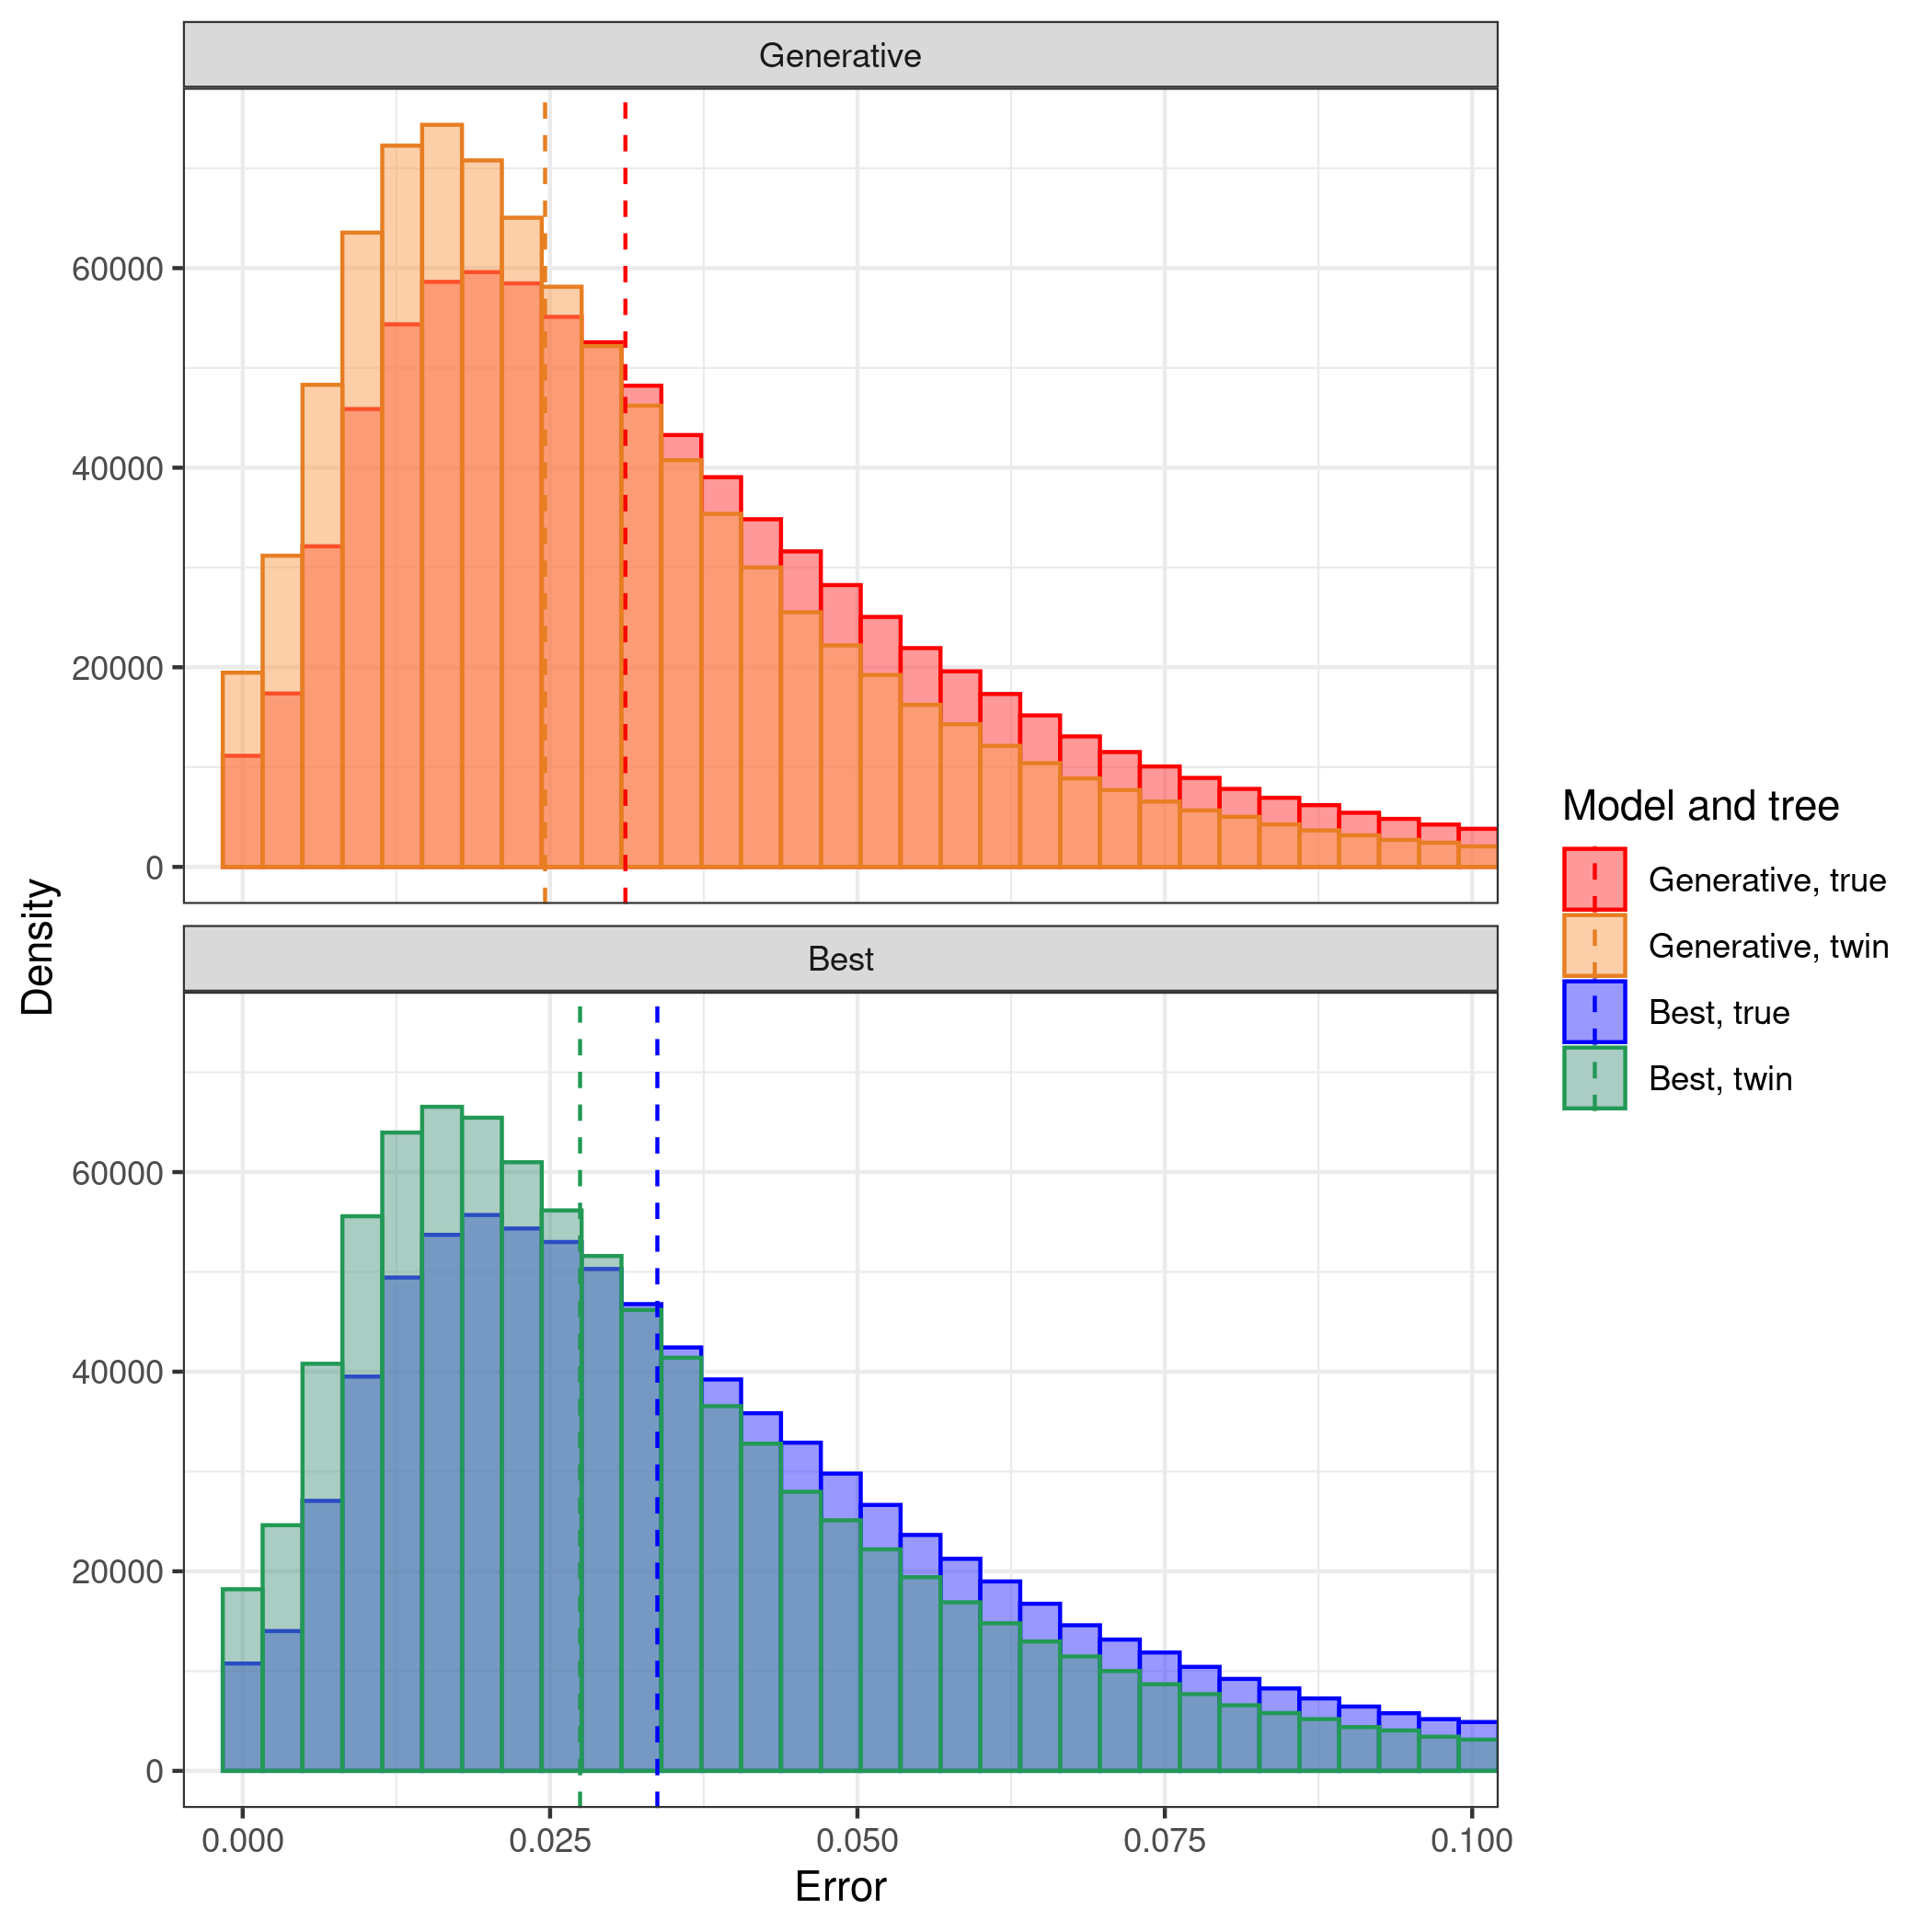
\includegraphics[width=\textwidth]{pirouette_example_38/errors.png}
  \caption{Aggregate error distributions for the tree distribution presented in \ref{subsec:distribution} but with a per-nucleotide mutation rate of 1.25 / crown age. This took 17 hours to compute.}
\end{figure}

\begin{figure}[H]
  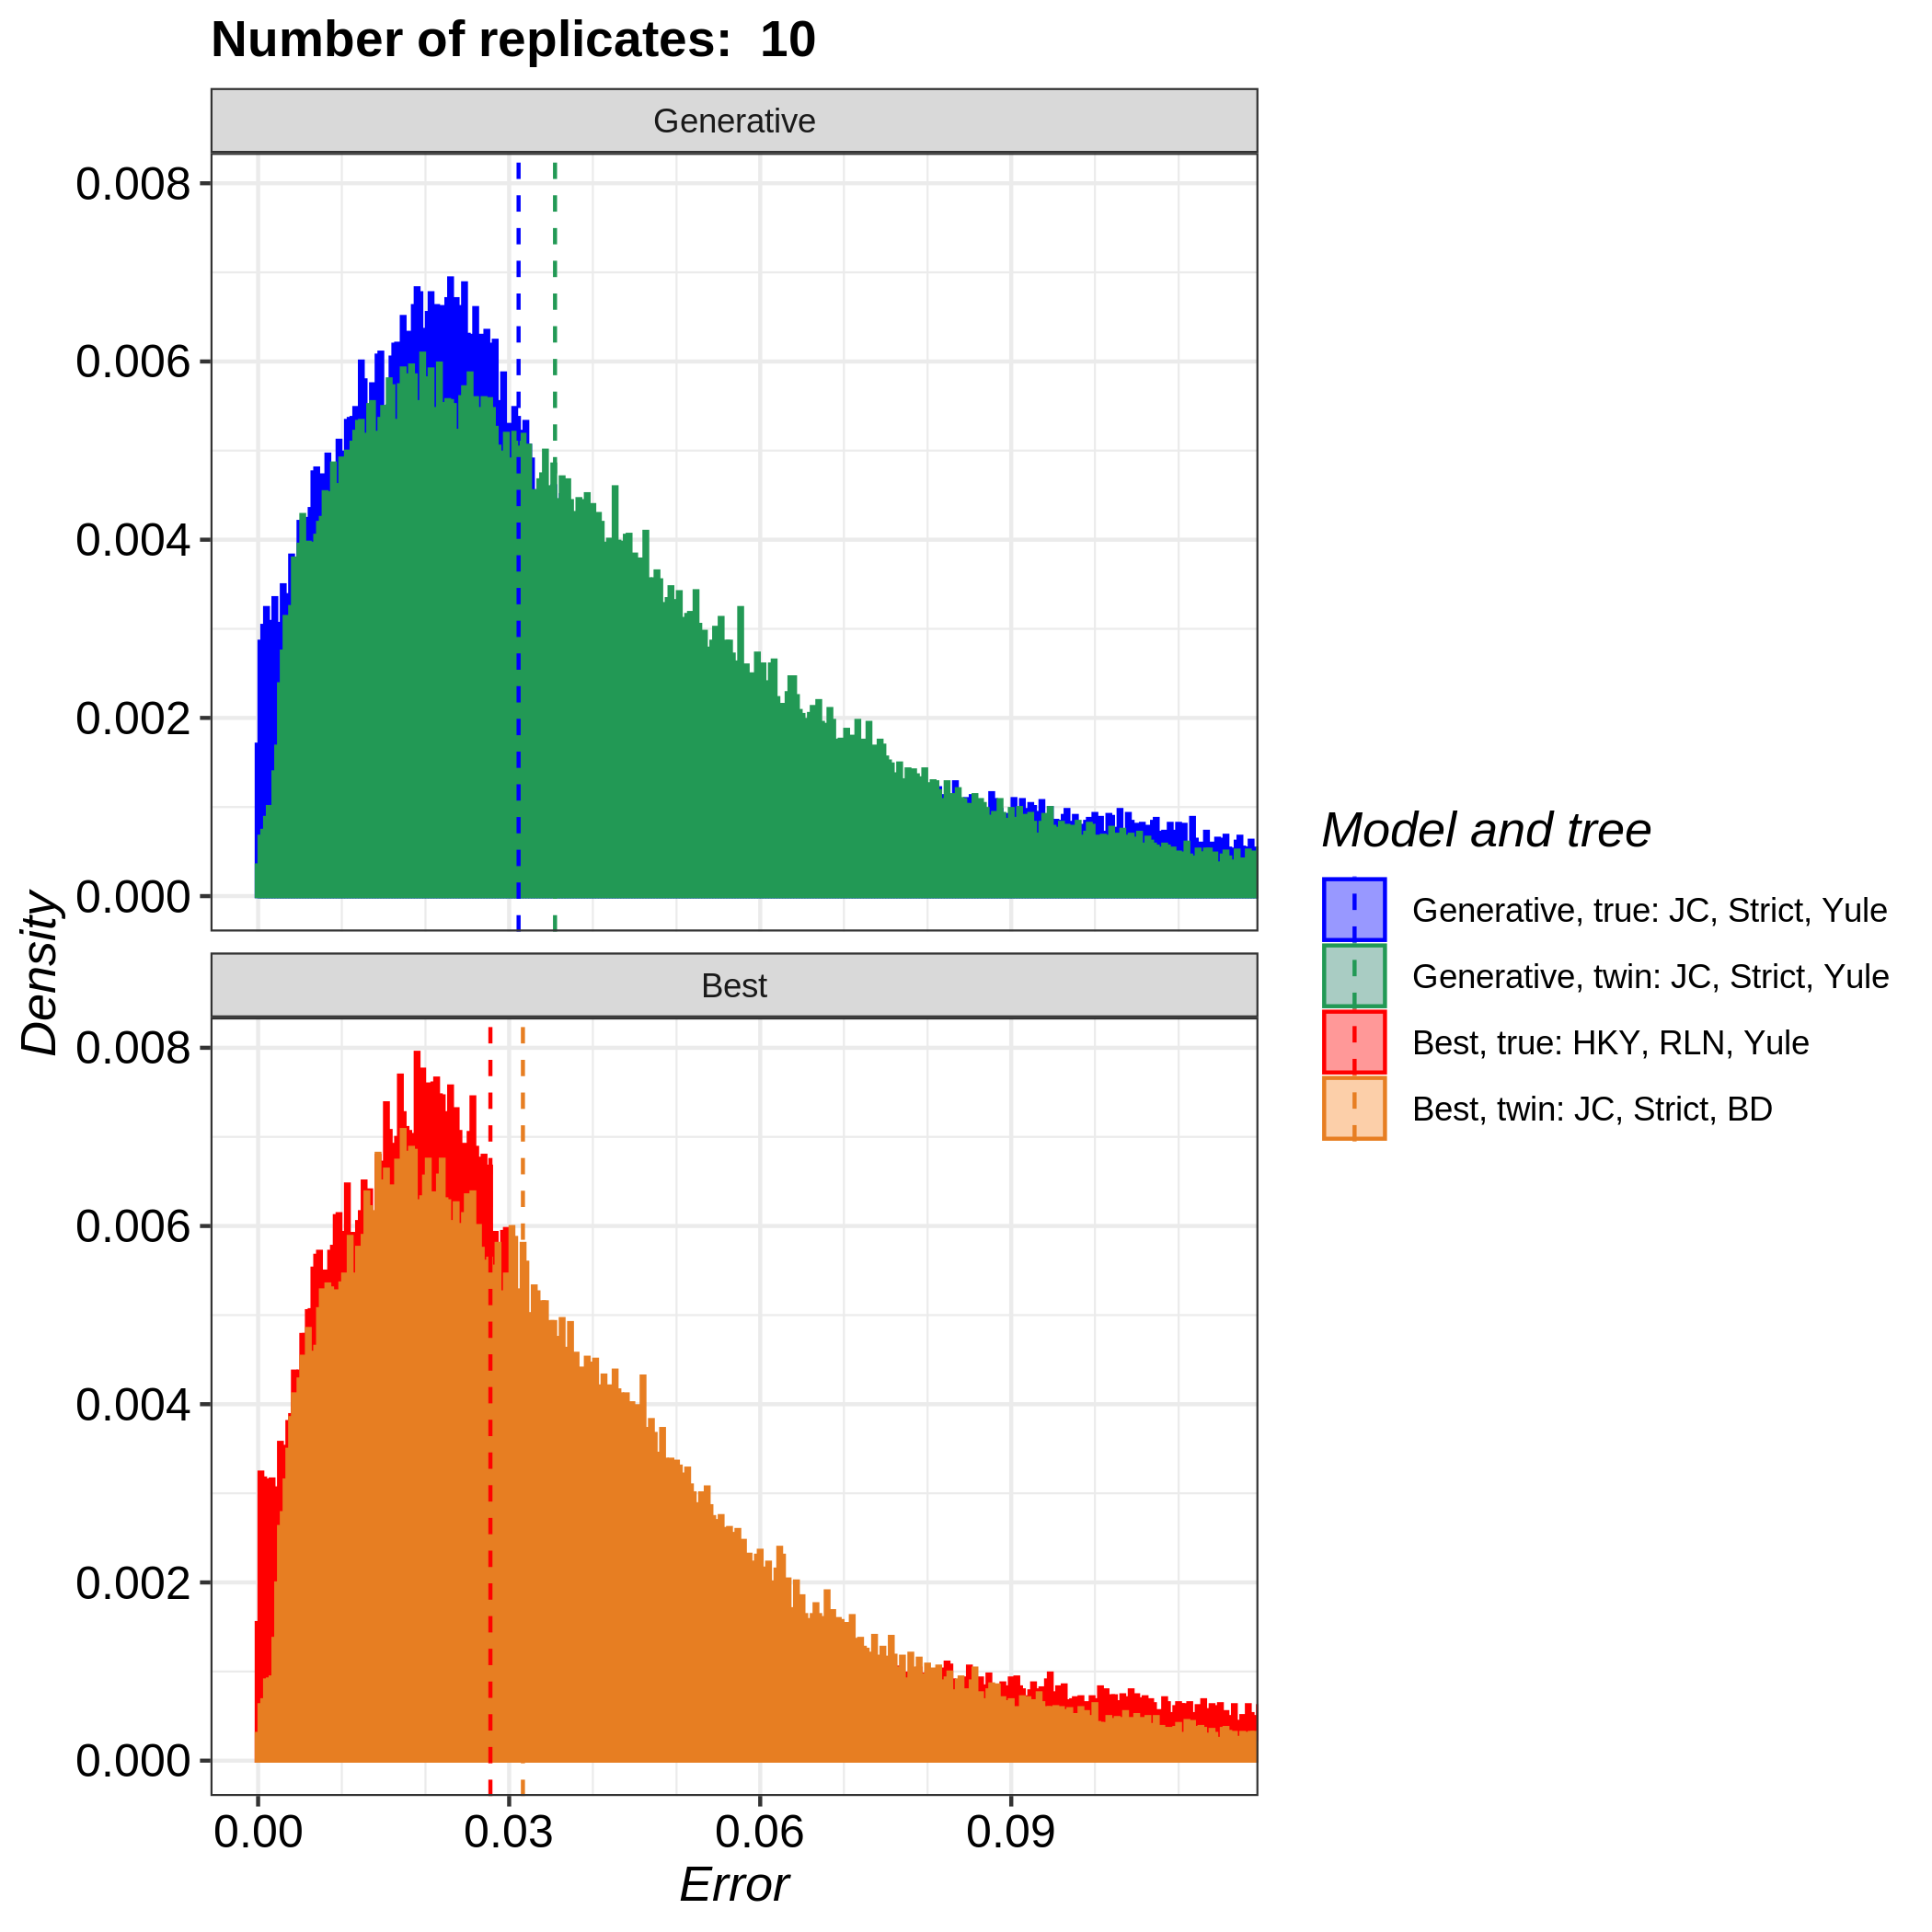
\includegraphics[width=\textwidth]{pirouette_example_39/errors.png}
  \caption{Aggregate error distributions for the tree distribution presented in \ref{subsec:distribution} but with a per-nucleotide mutation rate of 1.50 / crown age. This took 10 hours to compute.}
\end{figure}

\begin{figure}[H]
  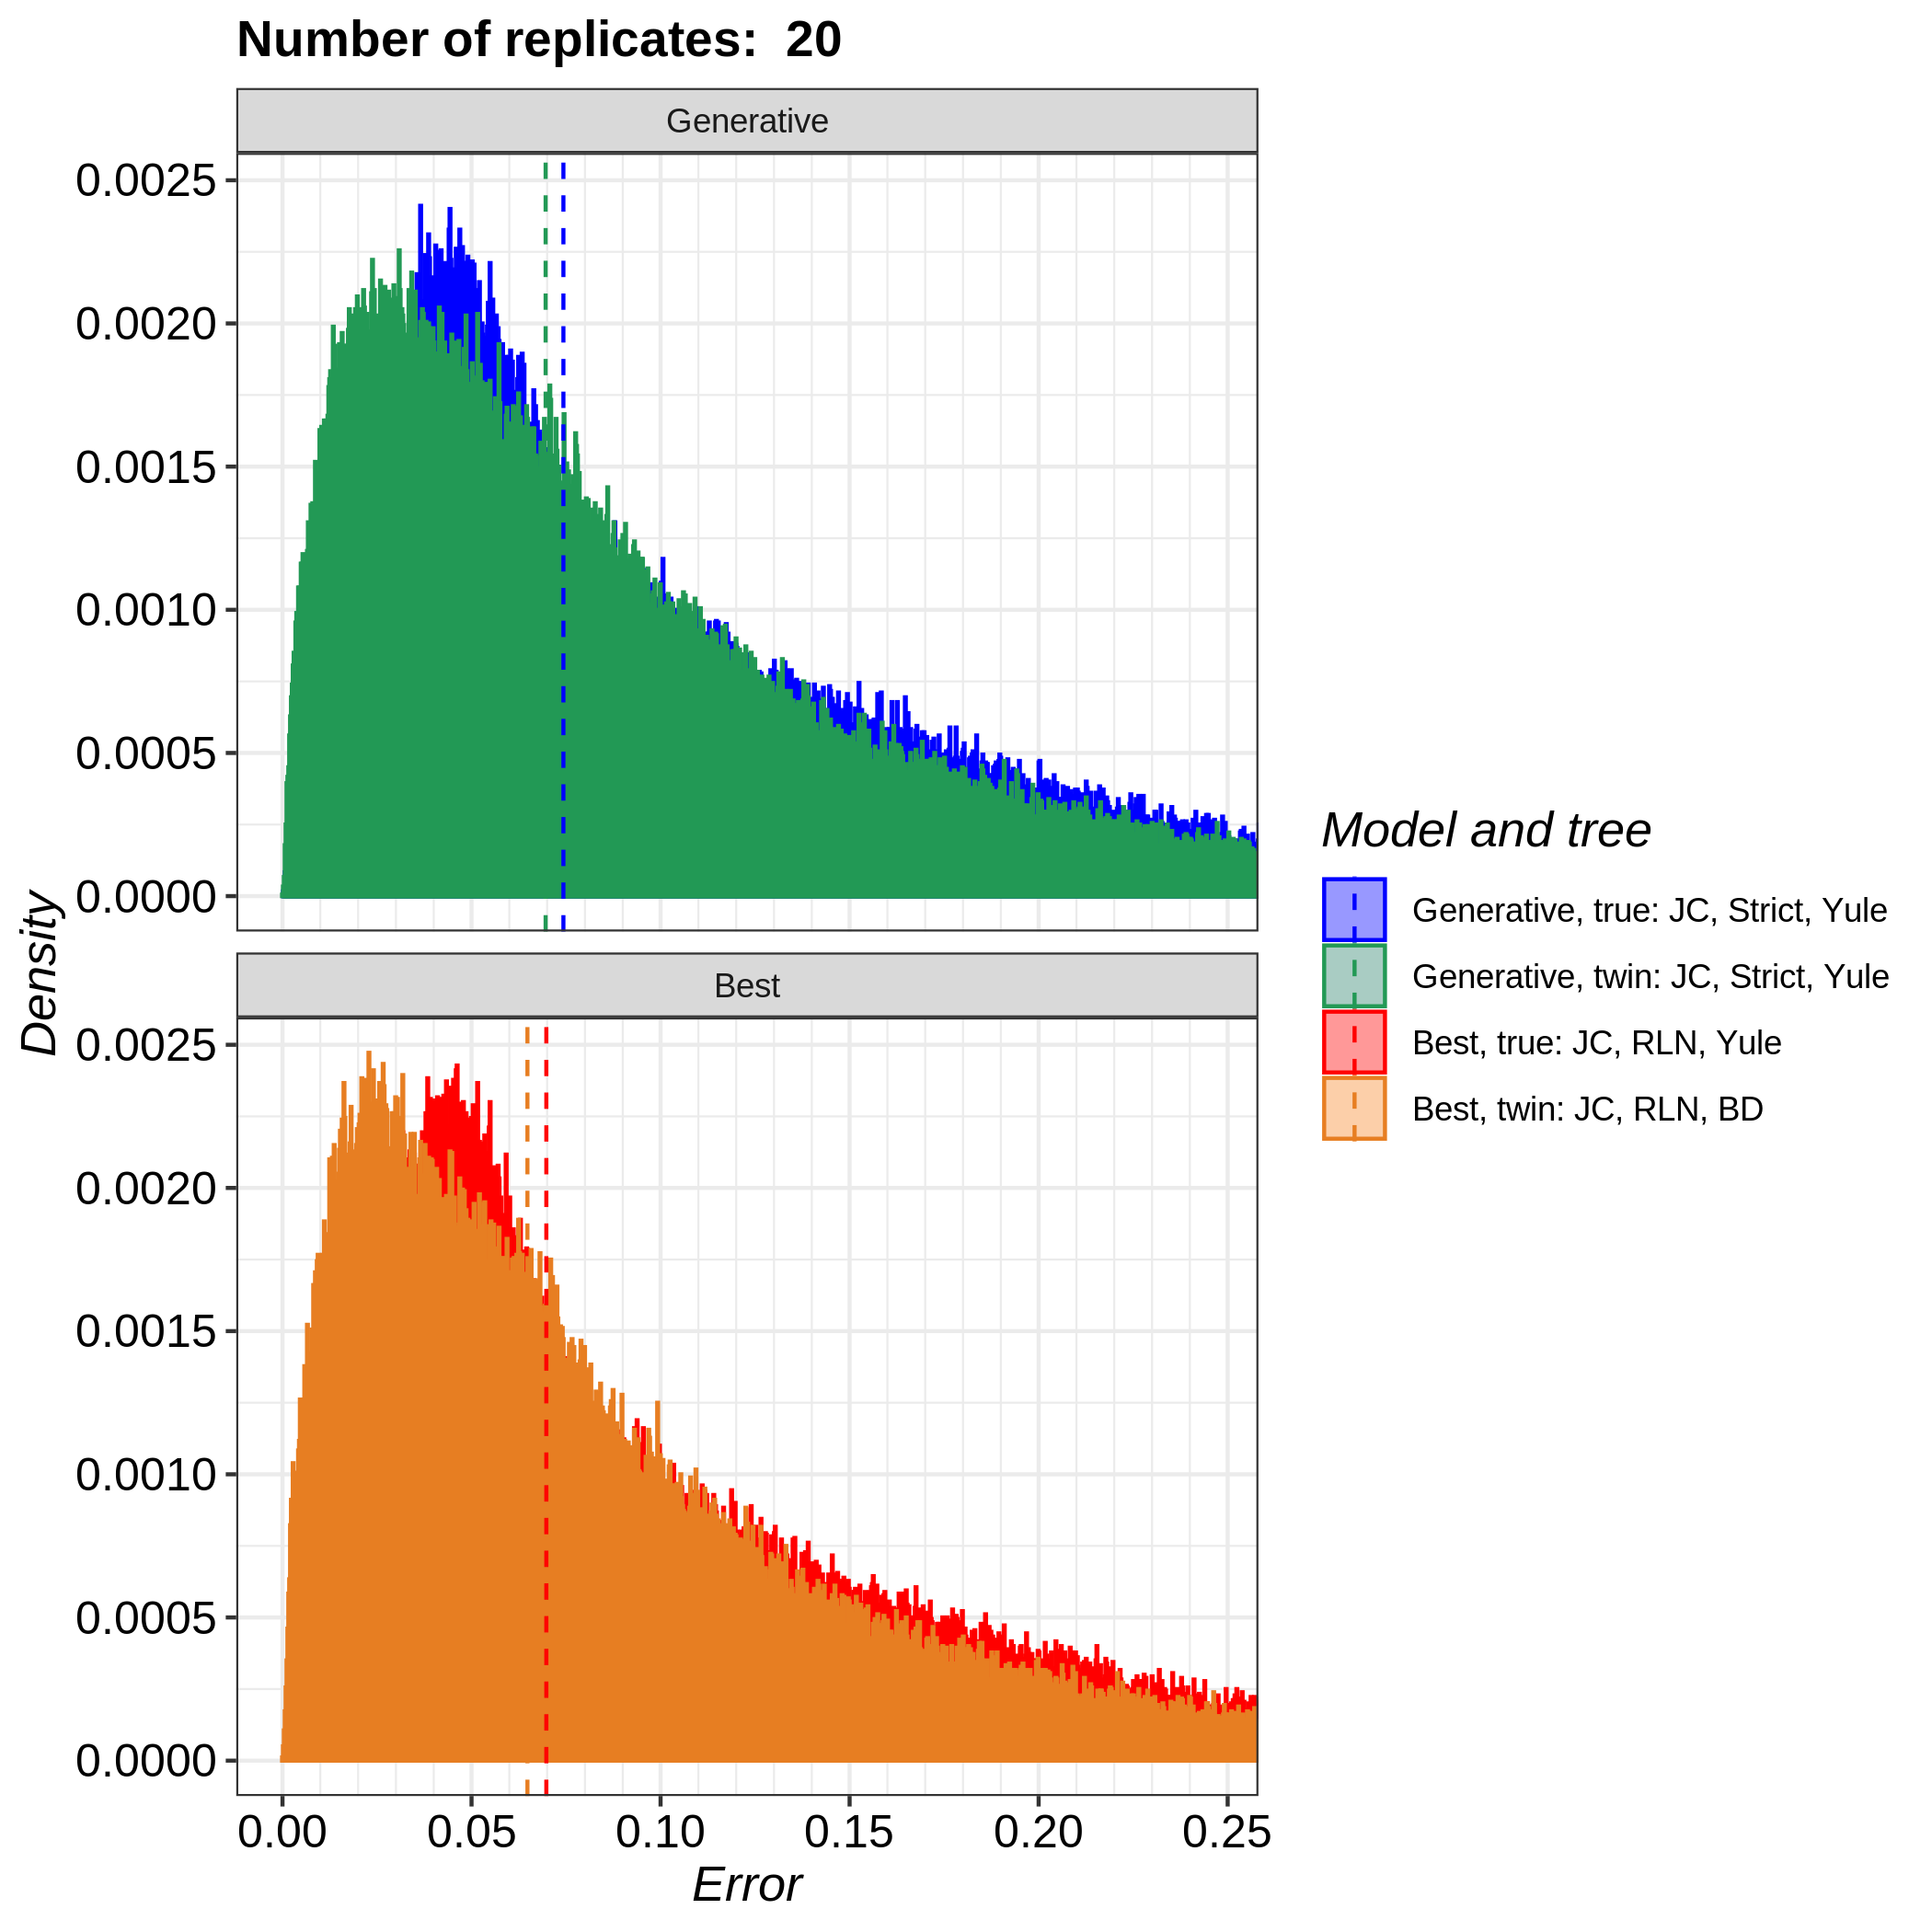
\includegraphics[width=\textwidth]{pirouette_example_40/errors.png}
  \caption{Aggregate error distributions for the tree distribution presented in \ref{subsec:distribution} but with a per-nucleotide mutation rate of 2.0 / crown age. This took 19 hours to compute.}
\end{figure}

%%%%%%%%%%%%%%%%%%%%%%%%%%%%%%%%%%%%%%%%%%%%%%%%%%%%%%%%%%%%%%%%%%%%%%%%%%%%%%%%
% Bibliography
%%%%%%%%%%%%%%%%%%%%%%%%%%%%%%%%%%%%%%%%%%%%%%%%%%%%%%%%%%%%%%%%%%%%%%%%%%%%%%%%
% MEE style
\bibliographystyle{pirouette_mee}
\bibliography{pirouette_supplement}
%%%%%%%%%%%%%%%%%%%%%%%%%%%%%%%%%%%%%%%%%%%%%%%%%%%%%%%%%%%%%%%%%%%%%%%%%%%%%%%%

